\documentclass[book,10pt]{book}
\input cmd.tex
\usepackage{url}
\usepackage{amssymb}
\usepackage{epsfig}

\title{Bytecode Verification and its Applications}
\begin{document}
\renewcommand{\topfraction}{0.9}
\renewcommand{\textfraction}{0.05}
\renewcommand{\floatpagefraction}{0.75}

\maketitle
\tableofcontents

%1
\chapter{Introduction}

%2
\chapter{ Java bytecode language and its operational semantics} \label{opSem}
 
%\input BML/cmdBML.tex

\newcommand{\code}{\textit{code}}
\newcommand{\indexComp}{\textit{index}}





\section{Introduction} \label{bcsl}
This section presents a bytecode level specification language, called for short BML and a compiler from a
 subset of the high level Java specification language JML to BML. 

% motivation

 Before going further, we discuss what advocates the need of a low level specification language.
Traditionally, specification languages were tailored for high level languages.  
Source  specification allows to express complex functional or security properties about programs.
Thus, they are / can successfully be used 
for software audit and validation. Still, source specification in the context of mobile code does not help a lot for several reasons.


First, the executable / interpreted code  may not be accompanied by its specified  source. Second, it is more reasonable for the 
code receiver to check the executable code than its source code, especially if he is not willing to trust the compiler. 
Third, if the client has complex requirements and even if the code respects them, in order to establish them, 
the code should be specified. Of course, for properties like well typedness this specification can be inferred automatically,
but in the general case this problem is not decidable. 
Thus, for more sophisticated policies, an automatic inference will not work.

 It is in this perspective, that we propose to make the Java
bytecode benefit from the source specification by defining the BML language and a compiler from JML towards BML.    

% what does the language support?
 BML supports the most important features of JML. Thus, we can express functional properties of Java
 bytecode programs in the form of method pre and postconditions, class and object invariants, assertions
 for particular program points like loop invariants. To our knowledge BML does not have predecessors that are tailored 
 to Java bytecode.  

 In section \ref{BCSLprelim}, we give an overview of the main features of JML. A detailed overview of BML is given in section \ref{BCSLgrammar}.  
  As we stated before, we support also a compiler from the high level specification language JML into BML. The 
 compilation process from JML to BML is discussed in section  \ref{BCSLcompile}.
 The full specification of the new user defined Java attributes in which the JML specification is compiled is given in the appendix.




   
 \section{Related work} \label{relWorkWp}

%%%%%%%%%%%%%%%%%%%%%%%%%%%%%%%%%%%%%%%%%%%%%%%%%%%%%%%%%%%%
In the following, we review briefly the existing work related to program verification
 and more particularly program verification tailored to Java and Java bytecode programs. 


 Floyd is among the first to work on program verification using logic methods for unstructured program
 languages (see \cite{F67amp}). Following the Floyd's approach, T.Hoare gives a formal logic for program verification in \cite{Hoare69ABC} known
 today under the name Hoare logic. Dijkstra \cite{WPCDS} proposes then an efficient way for applying Hoare logic in
 program verification, i.e. he comes up with a weakest precondition (wp) and strongest postcondition (sp) calculi. 

Concerning bytecode validation, there exists several approaches depending on the kind of properties that one want to check for.
 
 Bytecode verification is concerned with establishing that a bytecode is well typed 
(every instruction is applied to operands of the correct type) and well formed 
(e.g. no jumps to an un-existing bytecode index), differently from the goals of the present
work where program correctness is defined in terms of functional correctness. The JVM, for example, 
is provided with a bytecode verifier. There is a lot of research work done in the domain 
and for a detailed overview of the state of the art one can look at~\cite{Ljbc}.  

As Java has been gaining popularity in industry since the nineties of the twentieth century,
it also attracted the research interest.   
Thus the nineties upto nowadays give rise to several verification tools tailored to Java
 based on Hoare logic. Among the ones that gained most popularity are
esc/java developed at Compaq \cite{escjava}, the Loop tool \cite{jacobs03java}, Krakatoa, Jack \cite{BRL-JACK} etc.   

Few works have been dedicated to the definition of a bytecode logic. May be the earliest work in the field of bytecode verification 
is the thesis of C.Quigley  \cite{Quigley03PLJ} in which Hoare logic rules are given for a bytecode like language. This work is limited 
to a subset of the Java virtual machine instructions and does not treat for example method calls,
 neither exceptional termination. The logic is defined by searching a structure in the bytecode control flow graph,
 which gives an issue to complex and weak rules.

The work by Nick Benton \cite{B04tlsj} gives a  typed logic for a bytecode language with stacks and jumps. 
The technique that he proposes checks at the same time types and specifications.
The language is simple and supports basically stack and arithmetic operations. Finally, a proof of correctness
w.r.t. an operational semantics is given.

Following the work of Nick Benton, Bannwart and Muller \cite{BM05plb} give  a Hoare logic rules
for a bytecode language with objects and  exceptions. A compiler from source proofs into bytecode proofs is also defined. 
As in our work, they assume that the bytecode has passed the bytecode verification certification. The bytecode logic aims to 
express functional properties. Invariants are inferred by fixpoint calculation.
However, inferring invariants is not a decidable problem.


In ~\cite{WildmoserN-ESOP05}, M. Wildmoser and T. Nipkow describe a framework for verifying Jinja (a Java subset) bytecode 
against arithmetic overflow.  The annotation is written manually, which is not comfortable, especially on bytecode. 
Here we propose a way to compile a specification written in a high level language, allowing specification to be written
 at source level, which we consider as more convenient. \todo{not well explained the verification technique they have}

 The Spec\# (\cite{BLS04sp}) programming system developed at Microsoft proposes a static verification framework where 
 the method and class contracts  (pre, post conditions, exceptional postconditions, class invariants) are inserted in the intermediate code . 
 Spec\# is a superset of the C\# programming language, with a built-in  specification language, 
 which proposes a verification framework (there is a choice to perform the checks either at runtime or statically). 
 The static verification procedure  involves translation of the contract specification into metadata which is attached to the intermediate code. 
 The verification procedure \cite{leinoWPUP} that is performed includes several stages of processing the bytecode program:  
 elimination of irreducible loops, transformation into an acyclic control flow graph,
 translation of the bytecode into a guarded passive command language program. Despite that here in our implementation we also
 do a transformation in the graph into an acyclic program, we consider that in a mobile code scenario
 one should limit the number of program transformations for several reasons.
 First, we need a verification procedure as simple as possible, and second every transformation must be proven correct which is not always trivial.      

% Another topic related to the present work is PCC.
%  PCC and the certifying compiler were proposed by Necula (see \cite{Necula97,ComNec,DesNecLee98}). PCC is an architecture for establishing trust in untrusted code 
% in which the code producer supplies a proof for correctness with the code. 
% The initial idea for PCC  was that the producer automatically infers annotation for properties like well typedness, 
% correct read/writes and automatically generates the proof for their correctness using the certifying compiler. 
% However, such properties guarantee that a program executes correctly w.r.t. to the semantics of the 
% abstract machine, but cannot guarantee if a program executes correctly w.r.t to a functional specification.
% The verification condition generator presented in the following is tailored to deal with functional properties.


 


 
 
 
 \subsection{Notation}\label{notation}
 In the following, if we have a function $f$ with  domain type  $A$ and range type $B$
 we note it with $f : A \rightarrow B$. If the function receives n arguments of type $A1 \ \ldots \ A2$ respectively
 and maps them to elements of type $B$
 we note the function signature with $f : A1 * ...*A2 \rightarrow B$.   
 Function updates of function $f$ with n arguments is denoted with $ \update{f}{x1 \ldots xn}{y} $ and the definition of such function is :
 $$  \update{f}{x1 \ldots xn }{y}(z1 \ldots zn) = 
    \left\{\begin{array}{ll}
                  y & if \ x1 = z1 \wedge ...\wedge xn = zn \\
		  f(z1 \ldots zn ) & else
           \end{array}\right.$$
 
 The function \isInListOnly  takes as arguments any list and an object and  returns \textit{true} if the object is in the 
 list and \textit{false} otherwise:
 $$ \isInListOnly : list \ A * A \rightarrow \mbox{ \rm \textit{bool}}$$
 

 For any type $A$, the function \addInListOnly takes as argument any list $l: list \ A$ and an object 
$o: A$ and returns a list $l1 $ such that $l1.head = o \wedge l1.tail = l$: 
 $$
  \addInListOnly : list \ \AllRefs * \AllRefs \rightarrow  list \ \AllRefs 
 $$
 
  %\newcommand{\isFieldOfOnly}{\mbox{ \rm \textit{isFieldOf}} \ }
 % \newcommand{\isFieldOf}[2]{\mbox{ \rm \textit{isFieldOf}}(#1, #2) }

 \subsection{Classes, Fields and Methods}\label{clazz}
 Java programs are a set of classes. As the JVM says \textit{ A class declaration specifies a new reference type and provides its implementation. \ldots
 The body of a class declares members (fields and methods), static initializers, and constructors. }
 In our formalisation, the set of classes is denoted with $\ClassSet$, the set of fields with $\FieldSet$, the set of methods $\MethodSet$.
 We define a domain for class names \ClassName, for field names \FieldName \ and for method names \MethodName respectively.

 An object of type \ClassSet \ is a tuple with the following components: list of field objects (\fields), which are declared in this class,
 list of the methods declared in the class (\methods), the name of the class (\className)   and the super class of the class (\superClass)  :


 $$ \begin{array}{l}
          \forall  \clazz : \ClassSet , \\
         \clazz = \left\{\begin{array}{ll} \fields   & :    list \FieldSet \\
                                          \methods   & :    list \MethodSet\\
					  \className & :   \ClassName \\
					  \superClass& :   \ClassSet
                    \end{array} \right\}
   \end{array} $$

 A field object is a tuple that contains the unique field id and a field type, as well as where as the class where it is declared :  
 $$ \begin{array}{l} \forall \fieldd : \FieldSet, \\
       \fieldd = \left\{\begin{array}{ll}  \fieldName & : \FieldName;\\
                                     \fieldType &  : \JavaType; \\
				     \declaredIn & : \JavaClass
                     \end{array} \right\}
   \end{array} $$
 We introduce a special field which stands for the number of components of any reference pointing to an array object and which does not belong to any class
 (the name of the object and its field  \fieldName \ have the same name ):
 $$  \length =  \left\{\begin{array}{ll}  \fieldName & = \length;\\
                               \fieldType  & = int; \\
			       \declaredIn & = \bottom
                     \end{array} \right\}$$
 
% We assume that for any two different fields $\fieldd_1$ and $\fieldd_2$ their names are different : 
% $$\fieldd_1 \neq \fieldd_2 \Rightarrow \fieldd_1.fieldName \neq  \fieldd_2.fieldName  $$

 A method has a unique method id ( \methodName), a return type (\retType),
 a list containing the formal parameter names and their types(\args), 
 the number of its formal parameters (\numArgs),
 list of bytecode instructions representing its body (\body)
 and the entry point instruction of the method (\entryPoint)
 (the instruction at which every execution of the method starts), 
 the exception handler table ( \excHandlerTable )

 $$ \begin{array}{l}  \forall \methodd: \MethodSet, \\
                     \methodd  = \left\{\begin{array}{ll}  \methodName & :\MethodName\\
						          \retType & :\JavaType\\
							  \args &  : (name * \JavaType) [] \\
							  \numArgs & : nat \\
							  \body &  : \bcIns [] \\
							  \entryPoint  &  : \bcIns\\
							  \excHandlerTable & : \ExcHandler []
                                     \end{array}  \right\}
     \end{array} $$
  
 We assume that for every method \methodd the entrypoint is the first instruction in the array of instructions 
 of which its body consists, i.e. $ \methodd.\entryPoint =\methodd.\body[0]  $.


 An object of type \ExcHandler \ contains information about the region in the method body that it protects, i.e. the start
 position (\pcStart) of the region and the end position ( \pcEnd ), about the exception it protects from (\exc),
 as well as what position in the method body the exception handler starts (\pcHandler) at.


 $$ \begin{array}{l}  \forall \excHH: \ExcHandler, \\
                     \excHH  = \left\{\begin{array}{ll} \pcStart & : nat\\
						          \pcEnd & : nat\\
							  \pcHandler &  : (name * type)[] \\
							  \exc & : \ClassSet_{exc} 
                                        \end{array}  \right\}
     \end{array} $$
 
% For getting the value of any of the attributes in a class, method or field object we use the notation \textit{ name of the object . name of the attribute }
  
 
 
\subsection{Program Types}\label{types}
 The types supported by our language are a simplified version
 of the types supported by the JVM.
 Thus, we have a unique simple type : the integer data type \Myint.
 The reference type (\AllRefs) stands for the simple reference types (\reff)
 and array reference types(\reffArr ) .
 The language does not support interface types, still it can be extended 
 with minor difficuties to interface types. 

  

$$ \begin{array}{ll}
          \JavaType & ::= \Myint \mid \AllRefs\\
          \AllRefs  & ::= \reff \mid \reffArr \\
	  \reff     & ::= \ClassSet \\
	  \reffArr  & ::= \JavaType[]	  
   \end{array}  $$


Every type has an associated default value which can be accessed via
the function \defaultValueOnly. The function is defined as follows
$$ \defaultValue{\anyType} = 
           \left\{\begin{array}{ll}
	      \Mynull & \anyType \in \AllRefs \\
	       0 &  \anyType = \Myint
	    \end{array}\right. $$

We define also a subtyping relation as follows:

$$\begin{array}{ll}
  \frac{}{ \subtype{C}{C}} &  
  \frac{   C2 = C1.\superClass  }{\subtype{C1}{C2}} \\  
  & \\
  \frac{ C3 = C1.\superClass \   \subtype{C3}{C2} }{ \subtype{C1}{C2} } &
  \frac{}{  \subtype{C1}{Object}} \\
  & \\
  \frac{   }{\subtype{C[]}{Object}} &  
  \frac{ \subtype{C1}{C2}}{\subtype{C1[]}{C2[]}} \\
  \end{array}$$
 
 


%\newtheorem{StateSubst}[StateTransition]{State after assignment}
\newtheorem{StateProp0}{Substitution Property for Expressions}
\newtheorem{StateProp1}[StateProp0]{Substitution Property for Formulas}
 % lemme
\newtheorem{UpdateStateSem}[StateProp0]{Definition}
%\newtheorem{FieldAtState}[StateTransition]{Interpretation of field functions in a state}
%\newtheorem{StateSatisfiesProp}[StateTransition]{Predicate holds in a state}


\newtheorem{AtState}{Definition}


\newtheorem{FormulaInterp}[AtState]{Definition}
\newtheorem{StateProp2}[AtState]{Substitution Property for Field Functions } %lemme


\subsection{State configuration}\label{def}
 In this section, we introduce the notion of state configuration.
 A state configuration \SetConfigs models the program state in particular execution
 program point by specifying what is the state of the memory heap, the stack and the stack counter, the values of the
 local variables of the currently executed method  and what is the instruction which is executed next. 
 
 We define two kinds of state configurations:
 $$\SetConfigs = \SetConfigInterm \cup \SetConfigFinal$$
 The set $\SetConfigInterm$ consists of method intermediate state configurations, which stand for a 
 \textit{not stuck state} in which the execution of the current method is not finished i.e.
 there is still another instruction of the method body to be executed.  
 The configuration $\config{\heap}{\counter}{ \stackOnly }{\locVarOnly}{\pc } \in \SetConfigInterm$ has the following elements:
               \begin{itemize}
                     \item the function \heap is a mapping from field function names to the corresponding field function and from 
		     references to objects in the memory heap.
	   
	             \item \counter is a variable that contains a natural number which stands for the number of
		     elements in the operand stack.  

		     \item \stackOnly  stands for the operand stack and which for any integer 
		     \texttt{ind} smaller than the operand stack counter \counter 
		     retruns the value \stack{\texttt{ind}}  stored in the operand stack at \texttt{ind}
		     positions of the bottom of the stack. \stackOnly is not defined for natural values
		     greater than the counter. A newly created stack is denoted with \newStack
	     

	             \item \locVarOnly is the array of local variables of a method
		     and for an index \texttt{i} returns the value $\locVar{i}$ which is stored at that 
		     index of the array
	
	            \item \pc stands for the program counter and contains the index of the instruction to be executed in the current state
	        \end{itemize}


 The elements of the set $\SetConfigFinal$ are the final states, states in which the current method execution is terminated and consists of 
 normal termination states ($\SetConfigFinalNorm$) and exceptional termination states ($\SetConfigFinalExc$):
 $$\SetConfigFinal =  \SetConfigFinalNorm   \cup \SetConfigFinalExc $$ 
 
 A method may terminate either normally (by reaching a return instruction) or exceptionally (by throwing an exception).
 
 \begin{itemize}
        \item  $\configFinalNorm{\heap}{\Res} \in \SetConfigFinalNorm $ which describes a \textit{normal final state}, i.e.
	       the method execution terminates normally. The normal termination configuration has the following components :
               \begin{itemize}
                      \item \heap \ reflects what is the heap state after the method terminated 
		      \item \Res \ stands for the return value  of the method
	       \end{itemize}

	\item  $\configFinalExc{\heap}{\Exc} \in \SetConfigFinalExc $ which stands for an \textit{exceptional final state} of a method,
	       i.e. the method terminates by throwing an exception. The exceptional configuration has the following components:
               \begin{itemize}
                      \item the heap \heap 
		      \item \Exc \ is a reference to the uncaught exception that caused the method termination
               \end{itemize}

 \end{itemize}
  
 We will use the notation $\configFinal{\heap}{\Final}$ for any configuration which belongs to the set  $\SetConfigFinal$. 
 In the next subsection, we define in terms of state configuration transition relation the operational semantics of
 our bytecode programming language.
 
 
 \index{\HeapSet}
\index{\heap}
\index{\heapArrays}
\index{\heapArrays} 
\index{\heapTypeOf}
\newtheorem{heapDef}{Definition}[section]

 \subsection{Modeling the object heap} \label{heap}
 An important issue for the modeling of an object oriented programming language and its operational semantics
 is the memory heap. The heap is the
 runtime data area from which memory  for all class instances and arrays is allocated. Whenever a new instance
 is allocated, the JVM returns a reference value that points to the newly created object. 
 We introduce a record type \HeapSet \ which models the memory heap. We do not take into account 
 garbage collection and thus, we assume that heap objects has an infinite memory space. 
 
 In our modeling, a heap consists of the following components:
 \begin{itemize}
       \item a component  named \heapFields \ which is a partial function that maps field
             structures (of type \FieldSet \ introduced in subsection \ref{clazz} ) into partial functions from references (\AllRefs)
	     into values (\Values).  
 

       \item  a component \heapArrays \ which is a partial function from the components of arrays  into their values

       \item  a component  \heapLocs  \ which stands for the  list of references allocated in the heap
              
      % \item  a component \heapTypeOf   \ is a partial function  which maps references to their dynamic type 
 \end{itemize}


 Formally, the data type \HeapSet \ has the following structure:



  $$ \begin{array}{l}
         
         \heap = \left\{\begin{array}{ll}  \heapFields  &  : \FieldSet \rightharpoonup (  \RefValues \rightharpoonup \Values) \\
                                           \heapArrays  &  : \RefValuesArr * nat \rightharpoonup \Values \\
					   \heapLocs    &  : list \ \RefValues \\
					  % \heapTypeOf  &  : \RefValues \rightharpoonup \AllRefs
                    \end{array} \right\}
   \end{array} $$


 Another possibility is to model the heap as partial function from locations to objects where objects contain a function from 
 fields to values. Both formalizations are equivalent, still we have chosen this model as it follows closely the
 verification condition generator implementation.

 In the following, we are interested only in  heap objects \heap \ for which the components
 \heap.\heapFields \ and \heap.\heapArrays \ are functions defined only for references from the proper
 type, i.e. well-typed and which are in the list of references of the heap \heap.\heapLocs{} and are not \Mynull, i.e. well-defined.
We give the following formal definition.
\begin{heapDef}\label{heap:wf}
We say that the heap \heap{} is well-formed if the following holds: 
  $$\begin{array}{l}
           \forall  \fieldd : \FieldSet,   \\
   \begin{array}{ll} 
   \Dom( \heap.\heapFields(\fieldd))  =    \{ \referenceOnly \mid &	
                \referenceOnly  \in \heap.\heapLocs  \wedge \\
 	        &  \referenceOnly \neq \Mynull\\
  	        & \subtype{ \heapTypeOf(\referenceOnly ) }{\fieldd.\declaredIn} \}  
     \end{array}
	  \\
 	  and  \\
 	  \begin{array}{ll}  \Dom (\heap.\heapArrays) = \{  \referenceOnly \mid 	&  \referenceOnly  \in  \heap.\heapLocs \wedge \\ 
 	  &  \referenceOnly \neq \Mynull\\
 	  &  0 \leq i < \heap.\heapFields( \length)( \referenceOnly)   \}  
     \end{array}
 	 
    \end{array}
   $$
\end{heapDef}
%old formulation
% $$\begin{array}{ll}
%          \forall  \fieldd : \FieldSet, \forall \referenceOnly \in \RefValues, &  \referenceOnly \in \Dom( \heap.\heapFields(\fieldd)) \ \bydef\\
%%%	  &  \referenceOnly  \in \heap.\heapLocs  \wedge \\
%	  &  \referenceOnly \neq \Mynull\\
%%	  & \subtype{ \heap.\heapTypeOf(\referenceOnly ) }{\fieldd.\declaredIn} \\
%	  and &  \\
%	  \forall \referenceOnly \in  \RefValuesArr, &  (\referenceOnly  , i ) \in \Dom (\heap.\heapArrays) \bydef\\
%	  &  \referenceOnly  \in  \heap.\heapLocs \wedge \\ 
%	  &  \referenceOnly \neq \Mynull\\
%	  &  0 \leq i < \heap.\heapFields( \length)( \referenceOnly)  
%	 
%   \end{array}
%  $$


% Also, we assume that the heap must contain well formed values. By this, we mean that the heap  maps any field object \todo{is this restriction ok? }
% \fieldd : \FieldSet \ which has a reference  type (i.e. the component \fieldd.\fieldType \ contains a reference type  )  
%into a function which may only return references which are already defined in the heap. The same condition is required for array references whose elements
%are references, i.e. the value of an array elements is either a reference defined in the heap or \Mynull. The next formalization expresses the restriction for field 
%functions : 

% $$\begin{array}{ll}
%          \forall  \fieldd : \FieldSet, & \forall \referenceOnly \in \RefValues, \\ 
%          & \fieldd.\fieldType \in \AllRefs  \wedge \\
%	  & \referenceOnly  \in  \Range( \heap.\heapFields(\fieldd))  \Rightarrow \\
%	  & \Myspace  \referenceOnly \in \heap.\heapLocs \vee \referenceOnly = \Mynull \\	  
%   \end{array}
%  $$
 



 % We define an operation \addNewLocationOnly \  which adds a new reference to the list of references in a heap.
 % The only change that the operation will cause to the heap \heap \ is to add
 % a new reference $\referenceOnly$ to the list of references of the heap \heap.\heapLocs:   

 % $$ \addNewLocationOnly : \HeapSet *  \AllRefs   \rightarrow \HeapSet $$

 % Formally, the operation is defined as follows: 
 % $$ \begin{array}{l}
 %           \addNewLocation{\heap}{\referenceOnly} = \heap' \iff^{def} \\
 %	      \\
 %   	      \referenceOnly \notin \heap.\heapLocs   \\ 
 % %	      \heap'.\heapLocs = \referenceOnly \assocList \heap.\heapLocs \wedge \\ 
 %	      \heap.\heapFields = \heap'.\heapFields \wedge \\
 %	      \heap.\heapArrays = \heap'.\heapArrays \wedge \\
 %	     
 %    \end{array}$$ 



 If a new object of class $\clazz$ is created in the memory,
 a fresh reference value $\referenceOnly$ different from \Mynull{}  which points to the newly created object is added in the heap \heap \ 
 and all the values of the field functions that correspond to the fields in class $\clazz$ 
 are updated for the new reference with the default values for their corresponding types.
 The function which for a heap \heap \ and a class type \clazz \ returns the same heap but with a fresh reference of
 type \clazz \ has the following name and signature:
 $$ \newRefOnly :  \heap \rightarrow \reff \rightarrow  \heap * \Ref $$

 The formalization of the resulting heap and the new reference is given by the following definition.
\begin{heapDef}{Operator for instance allocation}\label{heap:instAlloc}
 $$  \begin{array}{l}
            \newRef{\heap}{\clazz} = (\heap',\referenceOnly )    \bydef\\
	    \\
	    \referenceOnly \neq \Mynull \wedge \\ 
	    \referenceOnly \notin \heap.\heapLocs \wedge   \\ 
	    \heap'.\heapLocs = \referenceOnly \assocList \heap.\heapLocs \wedge \\ 
	    \heapTypeOf(\referenceOnly) = \clazz \wedge \\
	    %\heap'.\heapTypeOf := \update{ \heap.\heapTypeOf}{ \referenceOnly}{\clazz}  \wedge \\ 
            \begin{array}{ll}
	           \forall  \fieldd : \FieldSet, & \instanceFlds{\fieldd}{\clazz} \Rightarrow \\
                                                 & \Myspace \heap'.\heapFields := 
			                           \update{\heap'.\heapFields}{\fieldd}{\update{\fieldd}{\referenceOnly}{ \defaultValue{\fieldd.\fieldType }}} \wedge \\
      \end{array}
     \end{array} $$
\end{heapDef}

In the above definition, we use the function \instanceFldsOnly, which for a given field \fieldd \ and \clazz \ returns true if \fieldd \ is
an instance field of \clazz: 

$$
 \instanceFldsOnly : \FieldSet   \rightarrow \ClassSet \rightarrow bool 
$$

$$
 \begin{array}{l}
       \instanceFlds{\fieldd}{\clazz } = \\
       \left\{\begin{array}{ll}
                    true  & \fieldd.\declaredIn = \clazz \\
		    false & \clazz = \Object \wedge \fieldd.\declaredIn \neq \Object \\
		    \instanceFlds{\fieldd}{\clazz.\superClass} & else
       \end{array}\right.
 \end{array}
$$


Identically, when allocating a new object of array type whose elements are of type \anyType \ and length $l$, we obtain 
a new heap object  $\newArrRef{\heap}{\anyType \lbrack \ \rbrack  }{l} $ which is defined similarly to the previous case: 
$$ \newArrRefOnly :  \heap \rightarrow  \reffArr \rightarrow  \heap * refArr $$
\begin{heapDef}{Operator for array allocation}\label{heap:arrAlloc}
 $$  \begin{array}{l}
            \newArrRef{\heap}{\anyType\lbrack \ \rbrack}{l} = (\heap', \referenceOnly)      \iff^{def} \\
	    \\
	    \referenceOnly \neq \Mynull \wedge \\ 
	    \referenceOnly \notin \heap.\heapLocs \wedge   \\ 
	    \heap'.\heapLocs = \referenceOnly \assocList \heap.\heapLocs \wedge \\ 
	    \heapTypeOf( \referenceOnly ) = \anyType\lbrack \ \rbrack  \wedge \\ 
	    %\heap'.\heapTypeOf :=  \update{ \heap.\heapTypeOf}{ \referenceOnly}{\anyType\lbrack \ \rbrack  }  \wedge \\ 
            \heap'.\heapFields :=  \update{\heap'.\heapFields}{\length}{\update{\length}{ \referenceOnly}{ l }} \wedge  \\
	    \forall i, 0 \le i < l  \Rightarrow   \heap'.\heapArrays :=
            \update{\heap'.\heapArrays}{(\referenceOnly , i)}{ \defaultValue{\anyType }  } \\
	     
     \end{array} $$
\end{heapDef}


In the following, we adopt few more naming conventions which do not create any ambiguity.
 Getting the function corresponding to a field \fieldd{} in a heap \heap \ :
$ \heap . \heapFields ( \fieldd)$ is replaced  with $ \heap  ( \fieldd)$ for the sake of simplicity.
 
The same abbreviation is done for access of an element in an  array object referenced by the reference 
 \referenceOnly{} at index $i$ in the heap \heap. Thus, the usual denotation:
$ \heap . \heapArrays (\referenceOnly, i )$ becomes $ \heap(\referenceOnly, i )$.
 
 
% The list of references of the resulting heap $\newRef{\heap}{\clazz}$ and the heap \heap
% has the following property:

% $$  \intersect{\getLocations{\heap}}{\newRef{\heap}{\clazz}} = \lbrack \Ref{\clazz} \rbrack $$



 
   Whenever the  field $\fieldd$ for the object pointed by reference
 $\referenceOnly$ is updated  with the value \textit{val},
 the component \heap.\heapFields \ is updated:
 $$ \update{\heap.\heapFields}{\fieldd}{\update{\heap.\heapFields(\fieldd)}{\referenceOnly}{val}} $$  
 In the following, for the sake of clarity, we will use another lighter notation for a field update which do not imply any ambiguities:
 $$ 
  \update{\heap}{\fieldd}{\update{\fieldd}{\referenceOnly}{val}} 
 $$ 



 If in the heap \heap \ 
 the $i^{th}$ component in the array referenced by $\referenceOnly$ is updated with the new value \textit{val},
 this results in assigning in an update of the component \heap.\heapArrays:
 $$\update{\heap.\heapArrays}{(\referenceOnly , i)}{val} $$ 
 In the following, for the sake of clarity, we will use another lighter notation for an update of an array component
 which do not imply any ambiguities:
 $$ 
  \update{\heap}{(\referenceOnly , i) }{val} 
 $$ 

 
 

 
 \subsection{Registers}\label{register}
State configurations have an array of registers which is
 denoted with    
\locVarOnly. Registers are addressed by indexing and 
 the index of the first register  is 0. 
Thus, \locVarOnly(0) stands for the first register in the state configuration.
 An integer is be considered to be an index into the register array if and only if that integer is between zero and one less than the size of the register array.
Registers are used to pass parameters on method invocation. On static method
 invocation, any parameters are passed in consecutive registers starting from register \locVarOnly(0). The register \locVarOnly(0) is always used to pass a
 reference to the object on which the instance method is being invoked
 (\texttt{this} in the Java programming language). 
The other parameters are subsequently passed in consecutive registers starting at register at index 1.
 
 \subsection{The operand stack}

Like the JVM language, our bytecode language is stack based. This means that every method is supplied with a Last In First Out
 stack which is used for the method execution to store intermediate results.
The method stack is modeled by the partial function \stackOnly \ and the variable
\counterOnly keeps track of the number of the elements in the operand stack. 
 \stackOnly \ is defined for any integer \texttt{ind} smaller than the operand stack counter \counterOnly 
 and returns the value \stackOnly(\texttt{ind})  stored in the operand stack at \texttt{ind}
 positions of the bottom of the stack. When a method starts execution its operand stack is empty and we denote the empty stack
 with \newStack. Like in the JVM our language supports instructions to load values stored in registers or object fields and vice versa.
 There are also instructions that take their arguments from the operand stack \stackOnly, operate on them and push the result on the operand
 stack. The operand stack is also used to prepare parameters to be passed to methods and to receive method results.   
 
 \subsection{Program counter}\label{pc}
The last component of an intermediate state configuration is the program counter \pc. It contains the number of the instruction in the array of instructions
of the current method which must be executed in the state. 
 
 \section{Throwing and handling exceptions}\label{opSem:exc}

As the JVM specification states \textit{exception are thrown if a program violates the semantic constraints of the Java programming language,
 the Java virtual machine signals this error to the program as an exception. An example of such a violation is an 
attempt to index outside the bounds of an array. The Java programming language specifies that an exception will be thrown when
 semantic constraints are violated and will cause a nonlocal transfer of control from the point where the exception occurred to
 a point that can be specified by the programmer. An exception is said to be thrown from the point where it occurred and is said to be
 caught at the point to which control is transferred. A method invocation that completes because an exception causes transfer of
 control to a point outside the method is said to complete abruptly. Programs can also throw exceptions explicitly, using throw statements \ldots }

Our language supports an exception handling mechanism similar to the JVM one.
 More particularly, it supports  Runtime exceptions: 
 \begin{itemize}
   \item \NullPointerExc \ thrown if a null pointer is dereferenced
   \item \NegativeArraySizeExc \ thrown if an array is accessed out of its bounds
   \item \ArrIndexOutOfBoundExc \ thrown if an array is accessed out of its bounds
   \item \ArithExc \ thrown if a division by zero is done
   \item \ClassCastExc \ thrown if an object reference is cast to to an incompatible type
   \item \ArrStoreExc \ thrown if an object is tried to be stored in an array and the object is of incompatible type with type of the  array elements
\end{itemize}

The language also supports programming exceptions. Those exceptions are forced by the programmer, by a special intruction called \athrow. 
The modelization of the exception handling mechanism involves several functions. 
 The function \getStateAfterExc \ deals with bytecode instructions that may throw exceptions. The function returns the state 
 configuration after the current instruction during the execution of \methodd \ throws an exception of type $\mbox{\rm\texttt{E}}$. If the  method
 \methodd \ has an  exception handler which can handle  exceptions of type $\mbox{\rm\texttt{E}}$ thrown at the index of the current  instruction,
 the execution is not stuck and thus, the state configuration is an intermediate state configuration.
 If the method \methodd \ does not have an exception handler for dealing with exceptions of type $\mbox{\rm\texttt{E}}$ 
 at the current index, the execution of \methodd \ terminates exceptionally and the current instruction
 causes the method exceptional termination:

 
 $$\begin{array}{l}
          \getStateAfterExc : \SetConfigInterm * \excType * \ExcHandler[] \rightarrow \SetConfigInterm \cup \SetConfigFinalExc  \\
	  \\
	  \getStateAfterExc( \config{\heap}{\counterOnly}{\stackOnly}{\locVarOnly}{\pc}, \mbox{\rm\texttt{E}}, \pc, \excHH[] ) = \\
          \left\{\begin{array}{ll}
	        \config{\heap'}{0}{\update{\stackOnly}{0}{\referenceOnly}}{\locVarOnly}{\pcHandler} & \begin{array}{l}  
                                                                                                           \mbox{\rm if \ \findExcHandler{\mbox{\rm\texttt{E}}}{\pc}{\excHH[]}} \\
													   =\pcHandler 
												      \end{array}	   
													   \\
		& \\
		\configFinalExc{\heap'}{\locVarOnly}{\referenceOnly} & \begin{array}{l}     
		                                                             \mbox{\rm  if \ \findExcHandler{\mbox{\rm\texttt{E}}}{\pc}{\excHH[]} } \\
		                                                             = \bottom  
		                                                        \end{array}
	  \end{array}\right.\\
	  \\
        \mbox{\rm where }\\
	(\heap', \referenceOnly )= \newRef{\heap}{\mbox{\rm\texttt{E}}}
    \end{array}
 $$

 If an exception $\mbox{\rm\texttt{E}}$ is thrown by instruction at position $i$ while executing the method \methodd,
 the exception handler table  \methodd.\excHandlerTable \ will be searched for the first exception handler that can handle the exception. 
 The search is done by the function \findExcHandlerOnly. If there is found
 such a handler the function returns the index of the instruction at which the exception handler starts, otherwise it returns $\bottom$:
 $$ \begin{array}{l}
        \findExcHandlerOnly : \excType * nat * \ExcHandler[] \rightarrow nat \\
	\\
	\findExcHandler{ \mbox{ \rm \texttt{E}} }{\pc}{\excHH[]} = \\
	 \left\{\begin{array}{ll}
	     \excHH[m].\pcHandler & \begin{array}{l}
	          		          hExc \neq emptySet \Rightarrow
					  min( hExc ) = m
			            \end{array}	 \\
			   & \\
	     \bottom &  hExc = emptySet
	 \end{array}\right. \\
\\ 
 \rm{where } \\  
  hExc = \{ k  \mid  \begin{array}{l} 
                        \excHH[k] = (\pcStart,\pcEnd,\pcHandler, \mbox{\rm\texttt{E}}' ) \wedge  \\
                        \pcStart \leq \pc < \pcEnd \wedge \\
			 \subtype{\mbox{\rm\texttt{E}}}{\mbox{\rm\texttt{E}}'} 
                    \end{array} \}
   \end{array}	  
 $$
 
 


\section{Bytecode Language and its Operational Semantics} \label{opSem}
 The bytecode language that we introduce here corresponds to a representative subset of the Java bytecode language. 
 In particular, it supports object manipulation and creation, method invokation, as well as exception throwing and handling.
 In fig. \ref{opSem:bclang}, we give the list of instructions that constitute our bytecode
 language.
 
 \begin{figure}[h] 
      $$  \begin{array}{lll}
             \bcIns ::= & \ifCond & \\
	                & \mid \goto  & \\ 
			& \mid \return  &\\ 
			& \mid \arithOp  & \\ 
			& \mid \load & \\ 
			& \mid \store & \\
			& \mid \push & \\
			& \mid \pop & \\
			& \mid \dup & \\
			& \mid \iinc & \\
			& \mid \new & \\
			& \mid \newarray &  \\ 	
			& \mid \putfield  & \\
			& \mid \getfield  & \\
			& \mid \arrstore &  \\
			& \mid \arrload  & \\
			& \mid \arraylength  & \\
			& \mid \instanceof  & \\
			& \mid \checkcast &  \\
			& \mid \athrow  & \\
			& \mid \invoke  & \\
		%	& \mid \jsr  & \\
		%	& \mid \ret  & \\
	\end{array}$$
        \caption{Bytecode Language instructions }
        \label{opSem:bclang}
  \end{figure}  
 	 
 Note that the instruction \arithOp stands for any arithmetic instruction in the list  \instr{add}, \instr{sub}, \instr{mult}, 
 \instr{and}, \instr{or}, \instr{xor} , \instr{ishr}, \instr{ishl}, \instr{div}, \instr{rem} ).
 


% We introduce two special value for the program counter $\botNorm$ and  $\botExc$. 
% The program counter \pc is set to $\bottom^{norm}$ whenever the method execution 
% terminates normally, i.e. the execution reaches a \return instruction. 
% On the other hand \pc receives the value $\bottom^{exc}$ if an instruction is
% executed which terminates with an uncaught exception.
% The key word \result \ is a special variable that stores the value that the current method returns.  
% \todo{say more about exceptions: exception table, how the exception handler is searched in a separate section may be}
 
%The function \excIndex{ind}{ExcType} returns either the index of the exception handler that protects the instruction at index \texttt{ind} from exception 
% type  \texttt{ExcType}, or $\bottom^{exc}$ if such a handler does not exist:

% $$
% \excIndex{\mbox{ \rm ind} }{ \mbox{ \rm ExcType} } = 
%\left\{ \begin{array}{ll}
%   ind^{ExcType} & \mbox{ \rm if an exception handler for ExcType exists  } \\
%   \bottom &    \mbox{ \rm else } 
% \end{array}\right.
% $$

 We define the operational semantics of a single Java instruction in terms of
 relation between the instruction and the state configurations
 before and after its execution.

 \begin{StateTransition}[State Transition] \label{stateTrans} 
 If an instruction \bcIns in the body of method \methodd \ starts execution in a state with configuration  
 $\config{ \heap}{\counterOnly}{\stackOnly}{\locVarOnly}{ \pc}$ and
  terminates execution in state with configuration  $\config{ \heap'}{\counterOnly'}{\stackOnly'}{\locVarOnly'}{\pc'}$ we denote this by

  $$  {\scriptsize \methodd \vdash \bcIns : \config{ \heap}{\counterOnly}{\stackOnly}{\locVarOnly}{ \pc }   \stateTrans \config{ \heap'}{\counterOnly'}{\stackOnly'}{\locVarOnly'}{\pc'} } $$
 \end{StateTransition}

 We also define how the execution of a list of instructions change the state configuration in  which their execution starts.
 
 \begin{transClosStateTrans}[Transitive closure of a state transition relation] \label{stateTransClos}
    If the body of the method \methodd \ \methodd.\body starts execution in a state
    with configuration \\ $\config{ \heap}{\counterOnly}{\stackOnly}{\locVarOnly}{\pc}$ and there is an execution
    path from \method.\entryPoint \ to an instruction \method.\body[k] which is either a \return \ instruction or an 
    instruction which terminates execution with an uncaught exception and the configuration after its execution is 
    $\configFinal{ \heap'}{\locVarOnly}{\Final}$  we denote it with 
    $$ {\scriptsize \methodd \vdash \methodd.\body: \config{ \heap}{\counterOnly}{\stackOnly}{\locVarOnly}{ \pc } \stateTrans^{*} \configFinal{ \heap'}{\locVarOnly'}{\Final} }$$
 \end{transClosStateTrans}
 



 We first give the operational semantics of a method execution. The execution of method \methodd 
 is the execution of its body upto reaching a final state configuration:
 
 $$
 {\scriptsize  \frac{\begin{array}{l}
          \methodd \vdash  \methodd.\body :  
	                    \config{\heap}{\counterOnly}{\stackOnly}{\locVarOnly}{\pc} \stateTrans^{*} \configFinal{\heap'}{\locVarOnly'}{\Final}\\
	\end{array}	 
       }
       {\methodd :  \config{\heap}{\counterOnly}{\stackOnly}{\locVarOnly}{\pc} 
		   \stateTrans 
                   \configFinal{\heap'}{\locVarOnly'} {\Final} }}$$ \\


 

   
 Next, we define the operational semantics of every instruction. The operational semantics
 of an instruction states how the execution of an instruction affects the program state configuration 
 in terms of state configuration transitions defined in the previous subsection \ref{def}.
 Note that we do not model the method frame stack of the JVM which is not needed for our purposes. 

\begin{itemize}
       \item Control transfer instructions \\\\

        \begin{enumerate}
            \item Conditional jumps : \ifCond


        $$ 
           {\scriptsize \frac{ \mbox{ \rm \texttt{ cond}}( \stackOnlyParam{\counterOnly}, \stackOnlyParam{\counterOnly - 1}) } 			       		               
                      {\method \vdash \ifCond \ n : \config{\heap }{\counterOnly}{\stackOnly}{\locVarOnly}{\pc}
		                      \stateTrans 
				      \config{\heap}{\counterOnly - 2}{\stackOnly}{\locVarOnly}{n}} 
            }    $$
		$$ {\scriptsize
                 \frac{  not (\mbox{ \rm \texttt{ cond}}( \stackOnlyParam{\counterOnly}, \stackOnlyParam{\counterOnly - 1})) }		                             
                     {\methodd \vdash \ifCond \ n : \config{\heap}{\counterOnly}{\stackOnly}{\locVarOnly}{\pc} 
		                    \stateTrans 
                                    \config{\heap}{\counterOnly - 2}{\stackOnly}{\locVarOnly}{\pc + 1}} }
           $$
            

	    The condition \texttt{cond} = $\{ =, \neq, \le, <, >, \ge \} $ is applied to the stack top  \stackOnlyParam{\counterOnly} and the element below the stack top
	     \stackOnlyParam{\counterOnly -1}which must be of type \Myint. If the condition is true then the control is transfered to the instruction
	    at index \texttt{n}, otherwise the control continues at the instruction following the current instruction. The top two elements \stackOnlyParam{\counterOnly} and
            \stackOnlyParam{\counterOnly - 1}  of the stack top are popped from the operand stack.
 
        \item Unconditional jumps: \goto \\
            $${\scriptsize \frac{  }
	            {\methodd \vdash \goto \ n: \config{\heap}{\counterOnly}{\stackOnly}{\locVarOnly}{\pc} 
		                    \stateTrans 
                                    \config{\heap}{\counterOnly}{\stackOnly}{\locVarOnly}{ n}} }$$
				    
   
             Transfers control to the instruction at position \textit{n}.


      \item \return
        $$ {\scriptsize \frac{ } 
            {\methodd \vdash \return :\config{\heap}{\counterOnly}{\stackOnly}{\locVarOnly}{\pc} 
		                    \stateTrans 
                                    \configFinalNorm{\heap}{\locVarOnly}{\stackOnlyParam{\counterOnly}}}   }  $$

	    The instruction causes the normal termination of the execution of the current method \methodd.
	    The instruction does not affect changes on the heap \heap and the return result is contained in
	    the stack top element \stackOnlyParam{\counterOnly}
      \end{enumerate}

  \item Arithmetic operations 	
        
	   $${\scriptsize \frac{ 
	   \begin{array}{l}
	   \counterOnly' = \counterOnly - 1 \\
	   \stackOnly' = \update{\stackOnly} {\counterOnly-1}{\stackOnlyParam{\counterOnly} \ \rm{op} \ \stackOnlyParam{\counterOnly-1}} \\
	   \pc' = \pc + 1
	   \end{array}}
		   {\method \vdash  \op :\config{\heap}{\counterOnly}{\stackOnly}{\locVarOnly}{\pc} 
		          \stateTrans 
                          \config{\heap}{\counterOnly'}{\stackOnly' }{\locVarOnly}{\pc'} } } $$ 
		 
 
       Pops the values which are on the stack top \stackOnlyParam{\counterOnly}  and \stackOnlyParam{\counterOnly - 1}  at the position below and applies the arithmetic operation \texttt{op}
       on them. The stack counter is decremented and  the resulting  value on the stack top \stackOnlyParam{\counterOnly - 1} \ \rm{op} \ \stackOnlyParam{\counterOnly} is pushed on the stack
       top  \stackOnlyParam{\counterOnly - 1}. 
	\todo{case for arithmetic instructions that throw exception }

  \item Load Store instructions

      \begin{enumerate}
    
	\item \load
	$${\scriptsize \frac{ \begin{array}{l}
	                \counterOnly' = \counterOnly + 1\\
			\stackOnly' = \update{\stackOnly}{\counterOnly +  1}{ \locVar{i} } \\
			\pc' = \pc + 1
	          \end{array}
	    } 
	    {\method \vdash \load \ \mbox{ \rm i}  : \config{\heap}{\counterOnly}{\stackOnly}{\locVarOnly}{\pc} 
		  \stateTrans 
                  \config{\heap}{\counterOnly'}{\stackOnly'}{\locVarOnly}{\pc'}  } } $$ 
            The instruction increments the stack counter  \counterOnly and pushes
	    the content of the local variable $\locVar{i}$ on the stack top \stackOnlyParam{\counterOnly + 1}
	    
        \item \store
        $$ {\scriptsize \frac{  \begin{array}{l}
	                \counterOnly' = \counterOnly- 1\\
			\locVarOnly' =	\update{\locVarOnly}{ \mbox{ \rm i} } { \stackOnlyParam{\counterOnly}} \\
			\pc' = \pc + 1
	          \end{array} }
                {\method \vdash  \store \ \mbox{ \rm i} :  \config{\heap}{\counterOnly}{\stackOnly}{\locVarOnly}{\pc} 
		  \stateTrans 
                  \config{\heap}{\counterOnly'}{\stackOnly }{\locVarOnly' }{\pc'} } } $$ 

	     Pops the stack top element \stackOnlyParam{\counterOnly}  and stores it into local variable $\locVar{\mbox{ \rm i}}$ and  decrements the stack counter 
	     \counterOnly  
	
        \item  \instr{iinc}

                $${\scriptsize  \frac{ \begin{array}{l}	               
			\locVarOnly' =  \update{\locVarOnly}{\mbox{ \rm i} }{ \locVar{\mbox{ \rm i} } + 1}\\
			\pc' = \pc + 1
	          \end{array} } 
	        {\method \vdash \instr{iinc } \ \mbox{ \rm i}  :  \config{\heap}{\counterOnly}{\stackOnly}{\locVarOnly}{\pc} 
		  \stateTrans 
                  \config{\heap}{\counterOnly}{\stackOnly}{\locVarOnly' }{\pc'}  }  } $$ 
            Increments the value of the local variable $\locVar{i}$ 
	
	\item \push
	       $${\scriptsize \frac{\begin{array}{l}
	                \counterOnly' = \counterOnly + 1\\
			\stackOnly' = \update{\stackOnly}{\counterOnly +  1}{\mbox{ \rm i}  }\\
			\pc' = \pc + 1
	          \end{array}  } 
	        {\method \vdash \instr{push} \ \mbox{ \rm i}  :  \config{\heap}{\counterOnly}{\stackOnly}{\locVarOnly}{\pc} 
		                                  \stateTrans  
						  \config{\heap}{\counterOnly + 1}{\stackOnly' }
						  {\locVarOnly}
						  {\pc'}  } } $$
     
      \item \instr{pop} 
       $${\scriptsize \frac{ } 
	        {\method \vdash \instr{pop}   :  \config{\heap}{\counterOnly}{\stackOnly}{\locVarOnly}{\pc} 
		                                  \stateTrans  
						  \config{\heap}{\counterOnly + 1}{\stackOnly}
						  {\locVarOnly}
						  {\pc + 1}  } } $$
    \end{enumerate}


   \item Object creation and manipulation 

     \begin{enumerate}

      \item \new \texttt{Cl}
            $${\scriptsize \frac{\begin{array}{l}
			(\heap',\referenceOnly) = \newRef{\heap}{\clazz} \\ 
			\counterOnly' = \counterOnly + 1\\
			\stackOnly' = \update{\stackOnly}{\counterOnly +  1}{ \referenceOnly  } \\
			\pc' = \pc + 1
	          \end{array}}
              {\method \vdash \new \ \clazz :  \config{\heap}{\counterOnly}{\stackOnly}{\locVarOnly}{\pc} 
		               \stateTrans  
			       \config{\heap'}
			              {\counterOnly'}
				      {\stackOnly' }
				      {\locVarOnly}
				      {\pc'}  } } $$
	      
	      A new fresh location $\referenceOnly$ is added in the memory heap \heap \ of type \\
               \clazz, the  stack counter \counterOnly is incremented.
	      The reference $\referenceOnly$ is put on the stack top \stackOnlyParam{\counterOnly + 1}. 
	


	\item \putfield  
           
	   $${\scriptsize \frac{ \begin{array}{l}
	               \stackOnlyParam{\counterOnly - 1} \neq \Mynull   \\
                       %\left\{\begin{array}{l}
		              \heap' = \update{\heap}{\fieldd }{\update{\fieldd}{\stackOnlyParam{\counterOnly - 1}}{\stackOnlyParam{\counterOnly }}} \\
			      \counterOnly' = \counterOnly - 2 \\
			      \pc' = \pc + 1
	               %\end{array}\right. \\
		      \end{array}   
		   }
                   { \methodd \vdash  \putfield \ \fieldd:  \config{\heap}{\counterOnly}{\stackOnly}{\locVarOnly}{\pc} 
                                               \stateTrans  
					       \config{\heap'}{\counterOnly'}{\stackOnly}{\locVarOnly}{\pc'} } } $$   

		     
	    
           $${\scriptsize \frac{ \begin{array}{l}
	                 \stackOnlyParam{\counterOnly - 1} = \Mynull   \\
		         \getStateAfterExc( \config{\heap}{\counterOnly}{\stackOnly}{\locVarOnly}{\pc}, \NullPointerExc, \methodd.\excHandlerTable ) =  \configVar			                  \end{array}
                      }
		      {\methodd \vdash  \putfield \ \fieldd:  \config{\heap}{\counterOnly}{\stackOnly}{\locVarOnly}{\pc} 
					          \stateTrans  
						  \configVar }} $$
						        
        The top value contained on the stack top \stackOnlyParam{\counterOnly} and the reference contained in \stackOnlyParam{\counterOnly - 1} 
	are popped from the operand stack. If \stackOnlyParam{\counterOnly - 1} is not \Mynull \footnote{here we assume that the code has passed successfully the bytecode verification procedure and thus,
	for instance, \stackOnlyParam{\counterOnly - 1} contains certainly a reference        of type \texttt{C}  } , the value of its field 
	\texttt{f} for the object  is updated 
	with the value\stackOnlyParam{\counterOnly} and the counter \counterOnly is decremented.
	If the reference in \stackOnlyParam{\counterOnly - 1} is \Mynull then a \NullPointerExc~ is thrown
          
        \item \getfield  
        	  
         $$ {\scriptsize \frac{ \begin{array}{l}
                               \stackOnlyParam{\counterOnly} \neq \Mynull \\
	                       %\left\{\begin{array}{l}             
			             \stackOnly' =  \update{\stackOnly}{\counterOnly}{ \heap(\fieldd)(\stackOnlyParam{\counterOnly} ) }\\
			             \pc' = \pc + 1
	                       %\end{array}\right.
	             \end{array}
                 }   
		 {\methodd \vdash  \getfield \ \fieldd  :  \config{\heap}{\counterOnly}{\stackOnly}{\locVarOnly}{\pc} 
						 \stateTrans  
						 \config{\heap}{\counterOnly}{\stackOnly'}{\locVarOnly}{\pc'}} } $$
			


        $${\scriptsize  \frac{ \begin{array}{l}
	                      \stackOnlyParam{\counterOnly} = \Mynull \\
			       \getStateAfterExc( \config{\heap}{\counterOnly}{\stackOnly}{\locVarOnly}{\pc}, \NullPointerExc, \methodd.\excHandlerTable ) =  \configVar                              \end{array}}
		  {\methodd \vdash  \getfield \ \fieldd  :  \config{\heap}{\counterOnly}{\stackOnly}{\locVarOnly}{\pc} 
						 \stateTrans  
						 \configVar} }$$
	 
	The top stack element \stackOnlyParam{\counterOnly}  is popped from the stack. If \stackOnlyParam{\counterOnly} is not \Mynull the value of the field \texttt{f}
	in the object referenced by the reference contained in \stackOnlyParam{\counterOnly}, is fetched and pushed onto the operand stack \stackOnlyParam{\counterOnly}.
        If \stackOnlyParam{\counterOnly} is \Mynull then a \texttt{NullPointerExc} is thrown, i.e. the stack counter is set to 0, a new object of type
	\texttt{NullPointerExc} is created in the memory heap store \heap and a reference to it $\Ref{NullPointerExc}$ is pushed onto the operand stack					 
			
        \item  \newarray  \ \anyType \\
	        $${\scriptsize \frac{\begin{array}{l}
		               \stackOnlyParam{\counterOnly} \geq 0  \\
			        %\left\{\begin{array}{l}
			                    (\heap',\referenceOnly ) = \newArrRef{\heap}{type}{\stackOnlyParam{\counterOnly}}\\
					    \counterOnly' = \counterOnly + 1\\
					    \stackOnly' = \update{\stackOnly}{\counterOnly +  1}{\referenceOnly } \\
					    \pc' = \pc + 1
			               % \end{array}\right.
			       \end{array}  }
                {\methodd \vdash  \newarray \ \anyType :  \config{\heap}{\counterOnly}{\stackOnly}{\locVarOnly}{\pc} 
		               \stateTrans  
			       \config{\heap'}
			              {\counterOnly'}
				      {\stackOnly' }
				      {\locVarOnly}
				      {\pc'}  } } $$

	  
	        $${\scriptsize \frac{\begin{array}{l}
		               \stackOnlyParam{\counterOnly} < 0 \\
			       \getStateAfterExc( \config{\heap}{\counterOnly}{\stackOnly}{\locVarOnly}{\pc}, \NegativeArraySizeExc,\methodd.\excHandlerTable ) =  \configVar                	        \end{array}  }
                {\methodd \vdash  \newarray \ \anyType :  \config{\heap}{\counterOnly}{\stackOnly}{\locVarOnly}{\pc} 
			                      \stateTrans  
					      \configVar } } $$
	  
	A new array whose components are of type \anyType \ and whose length is the stack top value is allocated on the heap.
	The array elements are initialised to the default value of  \anyType \ and a reference to it is put on the stack top. 
	In case the stack top is less than 0, then \NegativeArraySizeExc is thrown 

     
        \item \arrstore


      
	 $${\scriptsize \frac{ \begin{array}{l} 
	             \stackOnlyParam{\counterOnly - 2} \neq \Mynull  \\
		     0 \leq \stackOnlyParam{\counterOnly - 1  } < \length( \stackOnlyParam{\counterOnly - 2} )   \\
                     \heap' = \update{\heap}{( \stackOnlyParam{\counterOnly - 2},\stackOnlyParam{\counterOnly - 1} ) }{ \stackOnlyParam{\counterOnly}} \\
		     \counterOnly' = \counterOnly - 3 \\
		     \pc'  =  \pc + 1
		\end{array}}
		{\methodd \vdash  \arrstore \ :  \config{\heap}{\counterOnly}{\stackOnly}{\locVarOnly}{\pc} 
						 \stateTrans  
						 \config{\heap'}{\counterOnly'}{\stackOnly}{\locVarOnly}{\pc'}} } $$


       $${\scriptsize \frac{ \begin{array}{l}
	                      \stackOnlyParam{\counterOnly - 2} = \Mynull \\
			      \getStateAfterExc( \config{\heap}{\counterOnly}{\stackOnly}{\locVarOnly}{\pc} , \NullPointerExc,\methodd.\excHandlerTable ) =  \configVar  \\  
		   \end{array}}
		 {\methodd \vdash  \arrstore \ :  \config{\heap}{\counterOnly}{\stackOnly}{\locVarOnly}{\pc} 
			                         \stateTrans  
						 \configVar } } $$ 
        $${\scriptsize \frac{ \begin{array}{l} 
                                \stackOnlyParam{\counterOnly - 2} \neq \Mynull  \\
			  	( \stackOnlyParam{\counterOnly - 1} < 0 	\vee  \\
			       \stackOnlyParam{\counterOnly - 1} \geq \length (  \stackOnlyParam{\counterOnly - 2 }  ) ) \Rightarrow \\
			        \getStateAfterExc( \config{\heap}{\counterOnly}{\stackOnly}{\locVarOnly}{\pc}, \ArrIndexOutOfBoundExc ,\methodd.\excHandlerTable ) =  \configVar 
		    \end{array}}
		 {\methodd \vdash  \arrstore \ :  \config{\heap}{\counterOnly}{\stackOnly}{\locVarOnly}{\pc} 
			                         \stateTrans  
						 \configVar } } $$ 
	%Stores a value \stackOnlyParam{\counterOnly} \ at index \stackOnlyParam{\counterOnly - 1} \ in  the array component \stackOnlyParam{\counterOnly - 2}. 
	The three top stack elements \stackOnlyParam{\counterOnly}, \stackOnlyParam{\counterOnly - 1} \  and \stackOnlyParam{\counterOnly - 2} 
	are popped from the operand stack. The type value contained in \stackOnlyParam{\counterOnly} must be assignment 
	compatible\todo{say what assignment compatible is} with the type
	of the elements of the array reference contained in \stackOnlyParam{\counterOnly - 2},  \stackOnlyParam{\counterOnly - 1} \  must be of type int. 

	The value \stackOnlyParam{\counterOnly} \ is stored in the component at index \stackOnlyParam{\counterOnly - 1} \  of the array  in  \stackOnlyParam{\counterOnly - 2}.
	If \stackOnlyParam{\counterOnly - 2} \ is \Mynull a \NullPointerExc is thrown. If \stackOnlyParam{\counterOnly - 1}  \  is not in the bounds of the array 
	in \stackOnlyParam{\counterOnly - 2}  \ an \ArrIndexOutOfBoundExc exception is thrown. If \stackOnlyParam{\counterOnly} \ is not assignment 
	compatible with the type of the components of the array, then \ArrStoreExc  is thrown 

					 						 
\todo{one more case of exceptional termination if it terminates on an exception }


	\item \arrload       
	      
	     $${\scriptsize \frac{ \begin{array}{l}  \stackOnlyParam{\counterOnly - 1} \neq \Mynull  \ \\
					 \stackOnlyParam{\counterOnly} \geq 0   \\
					 \stackOnlyParam{\counterOnly} < \length (  \stackOnlyParam{\counterOnly - 1}  )  \\
			       			       %\left\{\begin{array}{l}
			                     \counterOnly' = \counterOnly - 1\\
					     \stackOnly' = \update{\stackOnly}{\counterOnly - 1} {  \heap(\stackOnlyParam{ \counterOnly -1 }{\stackOnlyParam{ \counterOnly} } ) } \\
					     \pc'  =  \pc + 1
			        %      \end{array} \right.
			 \end{array}}
			  {\methodd \vdash  \arrload \ :       \config{\heap}{\counterOnly}{\stackOnly}{\locVarOnly}{\pc} 
						 \stateTrans  
						 \config{\heap}{\counterOnly'}{\stackOnly'}{\locVarOnly}{\pc'}} } $$
						 

	  $${\scriptsize \frac{ \begin{array}{l}
	                      \stackOnlyParam{\counterOnly - 1} = \Mynull   \\
			      \getStateAfterExc( \config{\heap}{\counterOnly}{\stackOnly}{\locVarOnly}{\pc} , \NullPointerExc,\methodd.\excHandlerTable ) =  \configVar  \\  
		 \end{array}}
		 {\methodd \vdash  \arrload \ :  \config{\heap}{\counterOnly}{\stackOnly}{\locVarOnly}{\pc} 
			                         \stateTrans  
						 \configVar } } $$

                $$  {\scriptsize \frac{ \begin{array}{l}   
			      \stackOnlyParam{\counterOnly - 1} \neq \Mynull  \\
			      ( \stackOnlyParam{\counterOnly} < 0 	\vee  \\
			       \stackOnlyParam{\counterOnly} \geq \length (  \stackOnlyParam{\counterOnly - 1}  ) )   \\
			        \getStateAfterExc( \config{\heap}{\counterOnly}{\stackOnly}{\locVarOnly}{\pc}, \ArrIndexOutOfBoundExc ,\methodd.\excHandlerTable ) =  \configVar  
		    \end{array}}
		 {\methodd \vdash  \arrload \ :  \config{\heap}{\counterOnly}{\stackOnly}{\locVarOnly}{\pc} 
			                         \stateTrans  
						 \configVar } } $$					 						 
			
	       
	 

               Loads a value from an array. The top stack element \stackOnlyParam{\counterOnly} and the element below it \stackOnlyParam{\counterOnly -1 }
	       are popped from the operand stack.  \stackOnlyParam{\counterOnly} must be of type \Myint. The value in \stackOnlyParam{\counterOnly -1 } must be 
               of type \reff \ whose components are of type \textrm{type}. The value in the component of the array  \texttt{arrRef} 
	       at index \texttt{ind} is retrieved and pushed onto the operand stack.
	       If \stackOnlyParam{\counterOnly -1 } contains the value \Mynull a \NullPointerExc is thrown. If \stackOnlyParam{\counterOnly}  is
	       not in the bounds of the array object referenced by \stackOnlyParam{\counterOnly -1 }  a \ArrIndexOutOfBoundExc is thrown


    \item \arraylength
          $${\scriptsize \frac{ \begin{array}{l}
			   \stackOnlyParam{ \counterOnly } \neq \Mynull  \\
			    %\left\{\begin{array}{l}
			          \heap' = \heap \\ 
				  \counterOnly'= \counterOnly \\
				  \stackOnly'= \update{\stackOnly}{\counterOnly}{ \heap(\length)( {\stackOnlyParam{\counterOnly} } )  } \\ 
				  \pc' = \pc+ 1
                          % \end{array}\right.      
		    \end{array}
	        }
	        {\methodd \vdash \arraylength :  \config{\heap}{\counterOnly}{\stackOnly}{\locVarOnly}{\pc} 
		                  \stateTrans  
				  \config{\heap'}{\counterOnly'}{\stackOnly'}{\locVarOnly}{\pc'} } } $$
		     
	 

	  $$ {\scriptsize	 \frac{ \begin{array}{l}
			       \stackOnlyParam{ \counterOnly } = \Mynull    \\
			        \getStateAfterExc( \config{\heap}{\counterOnly}{\stackOnly}{\locVarOnly}{\pc}, \NullPointerExc ,\methodd.\excHandlerTable ) =  \configVar  
			\end{array}
		      }
		      {\methodd \vdash \arraylength : \config{\heap}{\counterOnly}{\stackOnly}{\locVarOnly}{\pc} 
		                                      \stateTrans  
						      \configVar} } $$
	The stack top element is popped from the stack. It must be a 
	reference that points to an array. If the stack top element \stackOnlyParam{\counterOnly} is not \Mynull  the length of the array  
	\length{\stackOnlyParam{\counterOnly} } is fetched and pushed on the stack.
	If the stack top element \stackOnlyParam{\counterOnly} is \Mynull then a \NullPointerExc is thrown.


	\item \instanceof
	      $${\scriptsize \frac{ \begin{array}{l}
                            \subtype{\heap.\heapTypeOf(\stackOnlyParam{\counterOnly})}{\clazz}  \\	
		           % \begin{array}{l}    
			          \stackOnly' = \update{\stackOnly}{\counterOnly}{1}   \\
                 		  \pc' =  \pc +1 
		           % \end{array}
			\end{array} 
	              }
                      {\instanceof  \ \clazz : \config{\heap}{\counterOnly}{\stackOnly}{\locVarOnly}{\pc} 
		                                   \stateTrans  
						   \config{\heap}{\counterOnly}{\stackOnly'}{\locVarOnly}{\pc'}} } $$
              
	      $$
	{\scriptsize	\frac{ \begin{array}{l}
                             not( \subtype{ \heap.\heapTypeOf( \stackOnlyParam{\counterOnly} ) }{\clazz}) \vee \stackOnlyParam{\counterOnly} = \Mynull  \\
			       %   \begin{array}{l}
			                \stackOnly' = \update{\stackOnly}{\counterOnly}{0}   \\
					\pc' =  \pc +1 
			  %    \end{array}
		        \end{array} }
		     {\methodd \vdash \instanceof  \ \tt{C} : \config{\heap}{\counterOnly}{\stackOnly}{\locVarOnly}{\pc} 
		                                   \stateTrans  
						   \config{\heap}{\counterOnly}{\stackOnly'}{\locVarOnly}{\pc'}}}  $$
		
	      
	      The stack top is popped from the stack. If it is of subtype \clazz or
	      is \Mynull, then the   \texttt{1} is pushed on the stack, otherwise \texttt{0}. 
         
       	\item \checkcast
          $${\scriptsize \frac{\begin{array}{l}
		               \subtype{\heap.\heapTypeOf( \stackOnlyParam{\counterOnly})}{\clazz }   \vee \stackOnlyParam{\counterOnly} = \Mynull  \\
			      \pc' =  \pc  +1 
		 \end{array}}
		  {\methodd \vdash \checkcast \ \clazz :     \config{\heap}{\counterOnly}{\stackOnly}{\locVarOnly}{\pc} 
		                             \stateTrans  
					     \config{\heap}{\counterOnly}{\stackOnly}{\locVarOnly}{\pc'}} }
	  $$	      
	  $${\scriptsize \frac{\begin{array}{l}	
			       not(\subtype{\heap.\heapTypeOf(  \stackOnlyParam{\counterOnly} ) }{\clazz} )  \\
			       \getStateAfterExc( \config{\heap}{\counterOnly}{\stackOnly}{\locVarOnly}{\pc}, \ClassCastExc,\methodd.\excHandlerTable ) =  \configVar                                              \end{array}}
		  {\methodd \vdash \checkcast \ \clazz :     \config{\heap}{\counterOnly}{\stackOnly}{\locVarOnly}{\pc} 
		                             \stateTrans  
					     \configVar} }  $$



	   The stack top is popped from the stack. If it is not of subtype \clazz \ an exception of type \ClassCastExc is thrown.

	 
   \end{enumerate}

   \item Throw exception instruction. \athrow
            $${\scriptsize \frac{ \begin{array}{l}	 
		             \stackOnlyParam{\counterOnly} \neq \Mynull   \\
			     \getStateAfterExc( \config{\heap}{\counterOnly}{\stackOnly}{\locVarOnly}{\pc},typeof( \stackOnlyParam{\counterOnly} )  ,\methodd.\excHandlerTable ) =  \configVar
		    \end{array}	     
	      }
              {\methodd \vdash \athrow :  \config{\heap}{\counterOnly}{\stackOnly}{\locVarOnly}{\pc} 
		                         \stateTrans  
					 \configVar} } $$

	     $${\scriptsize \frac{ \begin{array}{l}	 
	                     \stackOnlyParam{\counterOnly}  = \Mynull   \\
			     \getStateAfterExc( \config{\heap}{\counterOnly}{\stackOnly}{\locVarOnly}{\pc}, \NullPointerExc  ,\methodd.\excHandlerTable ) =  \configVar
      		    \end{array}	     
	      }
              {\methodd \vdash \athrow :  \config{\heap}{\counterOnly}{\stackOnly}{\locVarOnly}{\pc} 
		                         \stateTrans  
					  \configVar} } $$ 				 

           The stack top element  must be a reference of an object of type \\ \Throwable. 
	  If there is a handler that protects this bytecode instruction from the exception thrown, the control is transfered
	  to the instruction at which the exception handler starts\footnote{for every method the ExceptionHandler
	  table describes the corresponding exception handler by the limits of the 
	  region it protects, the Exception that it catches, and the instruction at which it starts}.
	  If the object on the stack top is \Mynull, a \NullPointerExc \ is thrown. 

 \item Method Invokation. \invoke \footnote{ only the case when  the invoked method returns a value}
      
         $$ {\scriptsize \frac{\begin{array}{l} \stackOnlyParam{ \counterOnly - meth.\numArgs } \neq \Mynull   \\
	                         meth : %\begin{array}{l} 
			                        \config{\heap}       
                                                       {0}
						       {\newStack }
                                                       {\lbrack \stackOnlyParam{ \counterOnly - meth.\numArgs },\ldots ,\stackOnlyParam{ \counterOnly} \rbrack }
						       {0} 
						         \stateTrans 
						\configFinalNorm{\heap'}{\locVarOnly'}{\Res}\\
				                %\end{array}  
                                                   \\
			  			 \\
			\left\{\begin{array}{l}
			       \counterOnly' = \counterOnly - \methodd.\numArgs + 1 \\
			       \stackOnly' = \update{\stackOnly}{\counterOnly'}{\Res} \\
			       \pc' = \pc + 1
			\end{array}\right. 
	         \end{array} 	      
	         }	         
	         {\methodd \vdash \invoke \  meth :  \config{\heap}{\counterOnly}{\stackOnly}{\locVarOnly}{\pc} 
		                        \stateTrans  
					\config{\heap' }{\counterOnly'}{\stackOnly' }{\locVarOnly}{\pc'}} } $$
	  
	  $${\scriptsize \frac{\begin{array}{l}
	                        \stackOnlyParam{ \counterOnly - meth.\numArgs } \neq \Mynull   \\
	                         meth: %\begin{array}{l} 
			                        \config{\heap}       
                                                       {0}
						       {\newStack }
                                                       {\lbrack \stackOnlyParam{ \counterOnly - meth.\numArgs },\ldots ,\stackOnlyParam{ \counterOnly} \rbrack }
						       {0} 
						         \stateTrans
						       \configFinalExc{\heap'}{\locVarOnly'}{\Exc}\\
				           %\end{array} \\
					   \Rightarrow \\
					  \getStateAfterExc( \config{\heap}{\counterOnly}{\stackOnly}{\locVarOnly}{\pc}, typeof(\Exc)  ,\methodd.\excHandlerTable ) =  \configVar
	         \end{array} 	      
	         }	         
	         {\methodd \vdash \invoke \  meth :  \config{\heap}{\counterOnly}{\stackOnly}{\locVarOnly}{\pc} 
		                        \stateTrans  
					\configVar} } $$


	  $${\scriptsize \frac{\begin{array}{l}
	                         \stackOnlyParam{ \counterOnly - meth.\numArgs } = \Mynull   \\ 
				 \getStateAfterExc( \config{\heap}{\counterOnly}{\stackOnly}{\locVarOnly}{\pc},\NullPointerExc,\methodd.\excHandlerTable ) =  \configVar
	         \end{array} 	      
	         }	         
	         {\methodd \vdash \invoke \  meth :  \config{\heap}{\counterOnly}{\stackOnly}{\locVarOnly}{\pc} 
		                        \stateTrans  
					\configVar} } $$					
	  

	 The first top $meth.\numArgs$ \ elements in the operand stack \stackOnly \ are popped from the operand stack. If 
         \stackOnlyParam{ \counterOnly - meth.\numArgs } is not \Mynull, the invoked method is executed on the object   \stackOnlyParam{ \counterOnly - meth.\numArgs } 
	 and where the first \numArgs + 1 elements of the list of its of local variables is initialised with \\
         \stackOnlyParam{ \counterOnly - meth.\numArgs } \ldots \stackOnlyParam{\counterOnly}. In case that the execution of method $meth$
	 terminates normally, the return value \Res \  of its execution is stored on the operand stack of the invoker. 
	 If the execution of of method $meth$ terminates because of an exception \Exc, then the exception handler of the invoker is searched for
	 a handler that can handle the exception. In case the object  \stackOnlyParam{ \counterOnly - meth.\numArgs } \  on which the  method $meth$ must be 
	 called is \Mynull, a \NullPointerExc is thrown.  			




% \item Subroutines
%    \begin{enumerate}
%          \item \jsr
% 	         $$\frac{ \begin{array}{l}
% 		                 \pc' =  \pc  + \it{ind} \\
% 				 pushJsr(\pc + 1)
%                            \end{array}  
% 		        } 
% 		     {\jsr \ \it{ind} : \config{\heap}{\counterOnly}{\stackOnly}{\locVarOnly}{\pc} 
% 		                        \stateTrans  
% 					\config{\heap}{\counterOnly}{\stackOnly}{\locVarOnly}{\pc'}}$$
% 	 \item  \ret
% 	        $$\frac{  \pc' =  getJsr() 
% 		          } 
% 			  {\ret : \config{\heap}{\counterOnly}{\stackOnly}{\locVarOnly}{\pc} 
% 		                        \stateTrans  
% 					\config{\heap}{\counterOnly}{\stackOnly}{\locVarOnly}{\pc'}}$$
%    \end{enumerate}

\end{itemize}


 


%4
\chapter{Specification language for Java bytecode programs} \label{bcsl}
  
%\input BML/cmdBML.tex

\newcommand{\code}{\textit{code}}
\newcommand{\indexComp}{\textit{index}}





\section{Introduction} \label{bcsl}
This section presents a bytecode level specification language, called for short BML and a compiler from a
 subset of the high level Java specification language JML to BML. 

% motivation

 Before going further, we discuss what advocates the need of a low level specification language.
Traditionally, specification languages were tailored for high level languages.  
Source  specification allows to express complex functional or security properties about programs.
Thus, they are / can successfully be used 
for software audit and validation. Still, source specification in the context of mobile code does not help a lot for several reasons.


First, the executable / interpreted code  may not be accompanied by its specified  source. Second, it is more reasonable for the 
code receiver to check the executable code than its source code, especially if he is not willing to trust the compiler. 
Third, if the client has complex requirements and even if the code respects them, in order to establish them, 
the code should be specified. Of course, for properties like well typedness this specification can be inferred automatically,
but in the general case this problem is not decidable. 
Thus, for more sophisticated policies, an automatic inference will not work.

 It is in this perspective, that we propose to make the Java
bytecode benefit from the source specification by defining the BML language and a compiler from JML towards BML.    

% what does the language support?
 BML supports the most important features of JML. Thus, we can express functional properties of Java
 bytecode programs in the form of method pre and postconditions, class and object invariants, assertions
 for particular program points like loop invariants. To our knowledge BML does not have predecessors that are tailored 
 to Java bytecode.  

 In section \ref{BCSLprelim}, we give an overview of the main features of JML. A detailed overview of BML is given in section \ref{BCSLgrammar}.  
  As we stated before, we support also a compiler from the high level specification language JML into BML. The 
 compilation process from JML to BML is discussed in section  \ref{BCSLcompile}.
 The full specification of the new user defined Java attributes in which the JML specification is compiled is given in the appendix.




 
  \newtheorem{defEdge}{Definition}[section]
\newtheorem{defLoop}[defEdge]{Definition}
\newtheorem{defInter}[defEdge]{Definition}
\newtheorem{defExc}[defEdge]{Definition}
\newtheorem{defInv}[defEdge]{Definition}
\newtheorem{defModif}[defEdge]{Definition}

\newtheorem{propPath}{Lemma}[section]

\section{Representing bytecode programs as control flow graphs}\label{prelim}

This section will introduce a formalization of an unstructured program in terms of a control flow graph.
The notion of a loop in a bytecode program will be also defined.
Performing analysis on programs written in  structured languages, is usually easier than performing the same analysis 
on unstructured programs. In particular, source loops in a method body correspond to a syntactic construction which is not the 
case for loops in methods on bytecode level. In order to discover a loop in a bytecode program we first need to define 
what is a bytecode program. Note that in the following, by a  bytecode program we mean a method body.

Every method \methodd \ has an array of bytecode instructions \methodd.\body \  which we already introduced in Section \ref{clazz}.
The $k-th$ instruction in the bytecode array $\methodd.\body$ is  denoted with $\methodd.\body[k]$.
 We assume that the method body has exactly one entry point
 (an entry point instruction is the instruction at which an execution of a method starts) which is the first
 element in the method body
$\methodd.\body[0]$.
The array of bytecode instructions of a method \methodd \ determine an oriented graph $G( V , \execRel ) $ in which the vertices are the instructions of the method body,
i.e. $$ V = \{ ins \mid \exists k,  0 \leq k < \methodd.\body.length \wedge ins = \methodd.\body[k] \}$$
The following definition defines the set of edges in the control flow graph.
\begin{defEdge}[Edge in control flow graph]\label{defEdge} 
 The set of edges $\execRel$ is a relation between the vertices elements
$$ \execRel : V * V $$ and is defined  as follows:
$$ \begin{array}{l} (\methodd.\body[j], \methodd.\body[k]) \in \execRel \\
   \iff \\
   \begin{array}{l} \methodd.\body[j] \neq \return \wedge( \\
                    \methodd.\body[j] = \ifCond \ k \vee \\
		    \methodd.\body[j] = \goto \ k \ \vee \\
		    \methodd.\body[j] \neq \goto \wedge  k = j+1 \ \vee \\ 
		    \methodd.\body[j] = \putfield \wedge \findExcHandler{ \NullPointerExc}{j}{\methodd.\excHandlerTable} = k \ \vee \\
		    \methodd.\body[j] = \getfield \wedge \findExcHandler{ \NullPointerExc}{j}{\methodd.\excHandlerTable} = k \ \vee \\
		    \methodd.\body[j] = \arrstore \wedge \findExcHandler{ \NullPointerExc}{j}{\methodd.\excHandlerTable} = k \ \vee \\
                    \methodd.\body[j] = \arrstore \wedge \findExcHandler{\ArrIndexOutOfBoundExc  }{j}{\methodd.\excHandlerTable} = k \ \vee \\
		    
		    \methodd.\body[j] = \arrload \wedge \findExcHandler{ \NullPointerExc}{j}{\methodd.\excHandlerTable} = k \ \vee \\
                    \methodd.\body[j] = \arrload \wedge \findExcHandler{\ArrIndexOutOfBoundExc  }{j}{\methodd.\excHandlerTable} = k \ \vee \\
		    \methodd.\body[j] = \invoke \ \mbox{\rm \texttt{n}} \wedge \findExcHandler{\NullPointerExc }{j}{\methodd.\excHandlerTable} = k \ \vee \\
		     \methodd.\body[j] = \invoke \ \mbox{\rm \texttt{n}} \wedge \forall \mbox{\rm\texttt{Exc}}, \exists s , \mbox{\rm \texttt{n}}.\exceptions[s ] = \mbox{\rm\texttt{Exc}} \wedge  \\
	\phantom{\methodd.\body[j] = \invoke } \findExcHandler{\mbox{\rm\texttt{Exc}} }{j}{\methodd.\excHandlerTable} = k \ \vee \\	    
		    \methodd.\body[j] = \athrow  \wedge \forall \mbox{\rm\texttt{Exc}}, \findExcHandler{\mbox{\rm\texttt{Exc}} }{j}{\methodd.\excHandlerTable} = k \ \vee \\
		    %\methodd.\body[j] = \athrow  \wedge \findExcHandler{\NullPointerExc }{j}{\methodd.\excHandlerTable} = k \vee 
		    
		    )
   \end{array} 
\end{array}$$
\end{defEdge}
From the Def. \ref{defEdge} follows that there is an edge between two vertices $\methodd.\body[j]$ and  $\methodd.\body[k]$ if they may execute immediately one after another.
 We say that $\methodd.\body[j]$ is a predecessor of $\methodd.\body[k]$ and that  $\methodd.\body[k]$ is a successor of  $\methodd.\body[j]$.
 The definition states the \return \  instruction  does not have successors.
If  $\methodd.\body[j ]$ is the jump instruction $ \ifCond \ k $ then  its successors are the instruction at index $k$ in the method body   
$\methodd.\body[k]$ and the instruction and the instruction $\methodd.\body[j + 1 ]$. 
From the definition, we also get that every instruction which potentially may throw an exception of type \texttt{Exc}
has as successor the first instruction of the exception handler that may handle the exception type \texttt{Exc}. For instance, a successor
of the instruction $\putfield$ is the exception handler entry point which can handle  the \NullPointerExc \ exception. 
The possible successors of the instruction $\athrow$ are the entry point of any  exception handler  in the method \methodd.
In the following, we will rather use the infix notation $\methodd.\body[j] \execRel \methodd.\body[k]$.
% We will also use the notation $\next{\methodd.\body[j] }$ for denoting the successor of   $\methodd.\body[j]$ in a given execution path.


We assume that the control flow graph of every method is reducible, i.e. every loop has exactly one entry point. This actually is admissible
as it is rarely the case that a compiler produce a bytecode with a non reducible control flow graph and the practice shows that even hand written
code is usually reducible. However, there exist algorithms to transform a non reducible control flow graph into a reducible one. 
For more information on program control flow graphs, the curious reader may refer to \cite{ARUCom1986}.
The next definition identifies backedges in the reducible control flow graph ( intuitively, the edge that goes 
from an instruction in a given loop in the control flow graph to the loop entry)  with the special execution relation $\execRel^l$ as follows:
 
\begin{defLoop}[Backedge Definition]
\label{defLoop}
Assume we have the method \methodd \ with body \methodd.\body \ which determine the control flow graph $G(V, \execRel) $.  We assume also 
that the entry point of $G$ is the vertice  $\methodd.\body[0]$.
 In such a graph $G$, we say that $\ins{loopEntry}$ is a loop entry instruction and $\ins{f}$ is a loop end instruction
 of the same loop if the following conditions hold:
\begin{itemize}
\item for every execution path $P$ from $\methodd.\body[0]$ to  $\ins{f}$:   $P~=~\methodd.\body[0] \execRel^{+} \ins{f}$
 there exists a subpath which is a prefix of $P$  $subP = \methodd.\body[0] \execRel^{*} \ins{loopEntry}$ such that $\ins{f} \notin  \ subP  $
%every path in the control flow graph starting at the entry point $\methodd.\body[0]$  that reaches $\ins{f}$, passes before reaching $\ins{f}$
% through  $\ins{loopEntry}$ 
\item there is a path in which $\ins{loopEntry}$  is executed immediately after the execution of $\ins{f}$ ( $\ins{f} \execRel \ins{loopEntry}$)
\end{itemize}
We denote the execution relation between $\ins{f}$ and  $\ins{loopEntry}$ with \\
$\ins{f} \execRel^l \ins{loopEntry}$ and we say that $  \execRel^l $  is a backedge. 
\end{defLoop}
We illustrate the upper definition with the control flow graph of the example from Fig. \ref{replaceSrc} in Fig. \ref{ctrlflow}.
In the figure, we rather show the execution relation between basic blocks which is a standard notion denoting a sequence of instructions which execute sequentially
and  where only the last one may be a jump and the first may be a target of a jump. 
The black edges represent a sequential execution relation, while dashed edges represent a backedge, i.e. the edge which stands for the execution
relation between a final instruction (instruction at index \texttt{18}) in the bytecode cycle and the entry instruction of the cycle (instruction at index \texttt{19}).  

% Note that from now on, we are interested in  control flow graphs with the following properties:

% \begin{itemize}
%  \item the control flow graph is reducible
 % \item an exception handler cannot be n
% \end{itemize}
 
\begin{figure}[ht!]
\begin{center}
%\includegraphics{bc.eps}
\epsfig{file=figs/bc.eps, height=5in,  width=1.5in}
\caption{{ \sc The control flow graph of the source program from Fig.\ref{replaceSrc}} }
\label{ctrlflow}
\end{center}
\end{figure}

%The next lemma states a property about execution paths in a control flow graph that contains backedges. This lemma will be used in the proof of correctness
% of our calculus in section \ref{proof}.
% \begin{propPath} \label{propPath}
% Let's have a control flow graph with an entry point instruction $\methodd.\body[0]$ and two instructions $\ins{loopEntry}$ and  
% $\ins{f}$ such that  \\
% $\ins{f}~\execRel^l~\ins{loopEntry}$. If there exists an execution path $P$ from $\methodd.\body[0]$ to  $\ins{f}$:   $P~=~\methodd.\body[0] \execRel^{+} \ins{f}$
% then there exists a subpath which is a prefix of $P$  $subP = \methodd.\body[0] \execRel^{*} \ins{loopEntry}$ such that $\ins{f} \notin  \ subP  $ 
% \end{propPath} 


%Once we have defined what a loop means in a control flow graph, we want also to define what a loop invariant means. 

%\begin{defInv}[Loop Invariant]\label{defInv}
%An invariant is an assertion which accompanies a backedge  in a bytecode control flow graph. Every backedge is accompanied 
%by an invariant. We denote an invariant with $\invariant$. If a backedge  $\execRel^{l}$ is accompanied by an invariant $\invariant$ 
%then $\invariant$ holds in every state in which an execution path passes through  the edge $\execRel^{l}$.    
%\end{defInv}

%We also assume that loop entries are provided with the locations \modifLoop \ that a loop may modify. 
%The interest of having the set of the locations that may be modified by a loop will be seen later when defining the weakest precondition
%predicate transformer.


% \begin{defModif}[Loop Modifies]\label{defModif} Every loop entry instruction $\ins{loopEntry}$ with
%a set of locations $\modifLoop = \{ mod_i \mid  i = 1 .. s\}$ whose meaning is the following: any two states $state_1, state_2 $  in which
% the instruction $ \ins{loopEntry}$ executes agree on local variables and the heap modulo the locations that are in the list \modifLoop.
%We denote the equality between  $state_1, state_2 $   modulo the modifies locations like this 
% $ state_1 =^{\modifLoop } state_2$
%\end{defModif}


  


% CHANGED - the example o compilation of loop specification

\newtheorem{bml}{Definition}[section]

\section{The subset of JML supported in BML} \label{BCSLgrammar}


BML corresponds to a representative subset of JML and is expressive enough for most purposes including the description of non trivial functional and 
 security properties. The following Section \ref{bml:notation} gives the notation conventions adopted here and 
Section  \ref{BCSL} gives the formal grammar of  BML as well as an informal description of its semantics. 

\subsection{Notation convention}\label{bml:notation}


\begin{itemize}
     \item Nonterminals are written with a \nonterminal font
     \item Terminals are written with a \terminal font
    % \item Keywords are writtem with a \keyWord font
     \item brackets  $\lbrack \ \rbrack $ surround optional text.
\end{itemize}


\subsection{BML Grammar}\label{BCSL}

%\begin{bml}[Formal grammar of BML]\label{BCSL} 
$$\begin{array}{ll}
     \Constants   & ::= \intLiteral  \mid \signedInt  \mid \Mynull \mid \ident  \\
     & \\

     \signedInt & ::= + \nonZeroDigit  \lbrack \digits \rbrack  \mid  - \nonZeroDigit  \lbrack \digits \rbrack \\

     & \\
     \intLiteral & ::= \digit \mid \nonZeroDigit  \lbrack \digits \rbrack \\

     & \\ 
     \digits & ::=  \digit  \lbrack \digits \rbrack \\

     & \\
     
     \digit & ::=  \mbox{\rm\textbf{0}} \mid \nonZeroDigit \\
     
     & \\

     \nonZeroDigit &::= \mbox{\rm\textbf{1}}  \mid \ldots \mid \mbox{\rm\textbf{9}}   \\
     
     & \\
     
     \ident & ::= \# \ \intLiteral \\    
     
     & \\
 
     \boundVar & ::= \ \bound\_\intLiteral \\ 

     & \\
    % \RefValuesSpec    & ::=  Ref \mid \Mynull \\
     & \\
    \expression      & ::= \Constants \\
                     &  \mid \locVar{ \digits } \\ 
       	             &  \mid \fieldAccess{\expression}{\ident} \\
		     &  \mid \ident \\
		  %  &  \mid  \update{\fieldd}{ \expression}{\expression}(\expression) \\
		     &  \mid \arrayAccess{\expression} {\expression} \\	   
		 %   &  \mid \update{ \arrayAccessOnly}{ (\expression , \expression)}{ \expression} (\expression,\expression) \\	
		     &  \mid \expression \ \op \ \expression   \\
		     &  \mid \counter \\
		     &  \mid \stack{ \expression} \\
                     &  \mid \old{ \expression  } \\
                     &  \mid \EXC    \\
		     &  \mid \result \\
		     &  \mid \boundVar \\
		     &  \mid \typeof{ \expression} \\
                     &  \mid \type{\ident} \\
                     &  \mid \elemtype{\expression  }\\
		     &  \mid \TYPE\\  
  & \\
 \op & ::=  \plus \mid \minus \mid \mult \mid \divis \mid  \modulo \\
 

    & \\
 \predicates & ::=  \  = \mid  \neq \mid \leq \mid \le \mid \geq \mid > \mid \subtypeSpec    \\
  & \\
 \formulaBc & ::= 
            \expression \ \predicates \  \expression   \\
	  & \mid  \true \\
	  & \mid  \false  \\	
          & \mid not \ \formulaBc  \\
	  & \mid \formulaBc  \wedge  \formulaBc \\
	  & \mid \formulaBc \vee  \formulaBc \\
	  & \mid \formulaBc  \Rightarrow \formulaBc \\
          & \mid \formulaBc \iff  \formulaBc \\
	  & \mid \forall \ \boundVar , \formulaBc\\
	  & \mid \exists \ \boundVar  , \formulaBc	 \\
    & \\
  \ClassSpec & ::=  \ClassInv \ \invModifier \  \formulaBc  \\
                 & \mid \ClassHistoryConstr  \ \formulaBc   \\
                 & \mid \declare \ \ghost \ \ident \ \ident \\  
   & \\
   
 \invModifier & ::= \instance \mid \static \\
		 
    & \\
  \intraMethodSpec & ::=  \begin{array}{l}  \atIndex \ nat; \\
		                            \intraSpec ; 
			  \end{array}\\
&\\
\intraSpec & ::=  \loopSpec \\ 
             & \mid \assert \ \formulaBc  \\                      
	     & \mid \set \ \expression \  \expression \\
& \\
\loopSpec  & ::=  \begin{array}{l}  
                        \loopInv \  \formulaBc; \\ 
			\loopMod \ list; \\ 
                        \loopDecreases \ \expression; 
	         \end{array}\\
    \end{array}$$


$$\begin{array}{ll} 
 %   & \\ 
  \MethodSpec & ::= \specCase \\     
                    & \mid  \specCase \ \also \ \MethodSpec \\

 & \\
  \specCase & ::=    \{| \\
                    & \phantom{aaa} \begin{array}{l}  
                              \requires  \ \formulaBc; \\
                                 \modifies  \ list \   \modifiesLoc;  \\
				 \ensures \ \formulaBc; \\
				 \exsuresList\\
				 
		     \end{array}  \\
                    &\phantom{aaa} |\} \\
 & \\ 
 \exsuresList & ::=   [ ] \mid  \exsures \ ( \ident )  \ \formulaBc  ; \exsuresList  \\
 & \\
  \modifiesLoc & ::=  \fieldAccess{\expression}{\ident} \\
                    & \mid \locVar{i} \\ 
                    & \mid \arrayAccessMod{\expression}{\specIndex}\\
		    & \mid \everything \\
		    & \mid \nothing \\
              
 & \\
 \specIndex & ::= \all \mid i_1 .. i_2 \mid i  \\
            
%\end{array}                
%$$

%$$ 
%\begin{array}{ll}    
 
%       & \\
%       \bmlKeyWords & ::= \requires \\
%                       & \mid \ensures \\
%		       & \mid \modifies \\
%		       & \mid \assert \\
%		       & \mid \set \\
%		       & \mid \exsures \\
%		       & \mid  \also \\
%		       & \mid  \ClassInv \\
%		       & \mid \ClassHistoryConstr \\
%		       & \mid \atIndex \\ 
%		       & \mid \loopInv \\
%		       & \mid \loopDecreases \\
%		       & \mid \loopMod \\
%		       & \mid \jmlKey{$\backslash$ typeof} \\
%		       & \mid \jmlKey{$\backslash$ elemtype}\\
%		       & \mid \TYPE\\
%		       & \mid \result 
\end{array}
$$


\subsection{Syntax and semantics of BML}

In the following, we will discuss informally the semantics of the syntax structures of BML.
Note that most of them have an identical counterpart in JML
 and their semantics in both languages is the same. 
 In the following, we will concentrate more on
 the specific syntactic features of BML and will just briefly comment
 the BML features which it inherits from JML like for instance, preconditions 
and which we have mentioned already\footnote{because we have already discussed  in Section \ref{BCSLprelim}
 the JML constructs for pre and postconditions, loop invariants, operators like \jmlKey{old}, \result, etc. we would not 
return to them anymore as their semantics is exactly the same as the one of JML}.  


\subsubsection{BML expressions}
Among the common features of BML and JML are the following expressions:
field access expressions $\fieldAccess{ \expression}{\ident}$, array access  
($\arrayAccess{\expression^1} {\expression^2} $),  arithmetic expressions
($\expression \ \op \ \expression$ ). Like JML, BML may talk about expression types.
As the BML grammar shows,  $ \typeof{\expression}$  denotes the dynamic type of the expression $\expression$, 
 $ \type{ \ident } $  is the class  described at index $\ident$ in the constant pool of the corresponding class file.
The construction $\elemtype{\expression}$ denotes the type of the elements of the array $\expression$,
and \TYPE, like in JML, stands for the Java type \texttt{java.lang.Class}. 

However, expressions in JML and BML differ in the syntax more particularly this is true for identifiers 
of local variables, method parameters, field and class identifiers. In JML, all these constructs
 are represented syntactically by their names in the Java source file. This is not the case in BML.

 We first look at the syntax of method local variables and parameters.
 The class file format stores information for them in the array of local variables.
 That is why, both method parameters and local variables are represented in BML 
 with the construct  $\locVar{i}$ which refers to the element at index $i$ in the array of local
 variables of a method. Note that the \texttt{this} expression in BML is encoded
 as $\locVar{0}$. This is because the reference to the current object is stored at index 0 in the array of local variables.

 
 Field and class identifiers in BML are encoded by the respective number in the constant pool table of the class file.
 For instance, the syntax of field access expressions  in BML is $\fieldAccess{\expression}{\ident}$ which 
 stands for the value in the field at index $\ident$ in the class constant pool 
 for the reference denoted by the expression  $ \expression $. 

 The BML grammar defines the syntax of identifiers differently from their usual syntax.
 Particularly, in BML those are positive numbers preceded by the symbol \# while usually
 the syntax of identifiers is a chain of characters which always starts with a letter. 
 The reason for this choice in BML  is that identifiers in BML are indexes in the constant
 pool table of the corresponding class.     

 Fig.\ref{bml:heavySpBML} gives the bytecode as well as the BML specification
 of the code presented in   Fig.\ref{bml:heavySp}. As we can see, the names of the local variables, field and class names  
 are compiled as described above.
 For instance, at line 3 in the specification we can see the precondition of the first specification case.
 It talks about $\locVar{1}$ which is the element in the array of local variables
 of the method  and which is the compilation of  the method parameter \texttt{b} (see Fig. \ref{bml:heavySp}). 

About the syntax of class names,  after the
 \exsures \ clause at line 5 follows a BML identifier (\#25) enclosed in parenthesis.
 This is the constant pool index at which the Java exception  type \texttt{java.lang.Exception} is declared.
 
\begin{figure}
\begin{lstlisting}[frame=trbl]

Class instance invariant: 
   lv(0).#19 > 0;
 

Method specification:
   {| 
    requires lv(1) > 0;
    modifies lv(0).#19;
    ensures  lv(0).#19 == \old( lv(0).#19 ) / lv(1);
    exsures  ( #25 ) false;  
   |}
   also 
   {|
    requires lv(1) == 0;
    modifies \nothing;
    ensures false;
    exsures ( #26 ) lv(0).#19  == \old(lv(0).#19);
   |}

 public void divide(int lv(1)) 
      0 load 0
      1 dup
      2 getfield #19 // instance field a
      3 load 1
      4 div
      5 putfield #19 // instance field a
      6 return
\end{lstlisting}
\caption{\sc An example for a heavy weight specification in BML} \label{bml:heavySpBML}
\end{figure}

%\begin{itemize}
%      \item  constants with the nonterminal 
%             $\Constants$. 
%             A constant is either a signed or unsigned integer, or an identier.  
%             Integers are defined in a standard way. Identifiers correspond 
%	     to indexes in the constant pool of a Java class and are always prefixed by the symbol $\#$. 
%             
%      \item  $\locVar{i}$ a local variable in the array of local variables of a method at index $i$.
%             Note that the array of local variables of a method in a class file
%             is the list containing both the formal parameters of the method and
%	     the variables declared locally in the method.
%             
%             
%      \item  field access expressions where $\fieldAccess{ \expression}{\ident}$ stands for accessing the field which 
%             is at index $\ident$ in the class constant pool of the class 
%             for the reference denoted by the expression  $ \expression $. 
%	      	    
%               
 %     \item  array access expression where $\arrayAccess{\expression^1} {\expression^2} $ stands for an access to the element at index $ \expression^2$ 
%             in the array denoted by the expression $ \expression^1$. This corresponds to the Java notation $\expression^1[\expression^2 ]  $ 
%             
%              
%      \item  $\expression \ \op \ \expression$ stands for the usual arithmetic operations 
%%             where $\op$ ranges over the standard  arithmetic operations $ + , - , * , div ,  rem $ 
%
%   
%      \item $\old{\expression}$  denotes the value of $\expression$ in the initial state of a method.
%            This expression makes sense in the postcondition of a
%            method and thus, allows that the postcondition predicate relate to the initial value of expressions.
%
%      \item $\EXC$ is a special specification identifier which denotes the thrown exception object in
%            exceptional postconditions
% \end{itemize}
%
A particular feature of BML is that it supports stack expressions which do not have a counterpart in JML.
These expressions are related to
 the way in which the virtual machine works, i.e. we refer to the stack and the stack counter.
Because intermediate calculations are done by using the stack, often we will need stack expressions in order to characterise the states before and after an instruction
execution. Stack expressions are represented in BML as follows:
\begin{itemize}
      \item  $\counter$ represents the stack counter.
      \item  $\stack{ \expression}$ stands for the element in the operand stack at position $\expression$.   
             For instance, the element below the stack top is represented with $\stack{\counter - 1}$ 
             % Differently from the JML, our bytecode specification language has to take into 
             % account the operand stack and its counter. 
	     Note that those expressions may appear in predicates that refer to intermediate instructions in the bytecode. 
	   
 \end{itemize}


%Finally, type expressions are given by the nonterminal $\typeExp$. 
%Note that all of these expressions have their analogue in JML and have the following meaning:
%\begin{itemize}
%   \item  $ \typeof{\expression}$  denotes the dynamic type of the expression $\expression$ 
%
%%      \item $ \type{ \ident } $  denotes the class  described at index $\ident$ in the constant pool of the corresponding class file
% 
%      \item $\elemtype{\expression}$ denotes the type of the elements of the array $\expression$
%      \item \TYPE.  This keyword stands for the Java type \texttt{java.lang.Class}\footnote{In the Java Application Programming Interface (API), 
%            instances of the class \texttt{java.lang.Class} represent Java classes, interfaces or basic types}. Notice that expressions
%	    $ \typeof{\expression}$, $\type{\ident}$ and $\elemtype{ \expression }$ are of type \TYPE.     
%
% \end{itemize}

\subsubsection{BML predicates}
 The properties that our bytecode language can express are from first order predicate logic. The formal grammar of the predicates is
 given by the nonterminal $\formulaBc$. From the formal syntax, we can notice that BML supports the standard logical connectors
 $\wedge, \vee, \Rightarrow $, existential $\exists$ and universal quantification $\forall$ as well as standard relation between
 the  expressions of our language like $\neq, = , \leq, \le \ldots$  
 

\subsubsection{Class Specification}
 The nonterminal  \ClassSpec \ in the BML grammar defines syntax constructs for the
 support of class specification. Note that these specification features exist in JML
 and have exactly the same semantics. 
 However, we give a brief description of the syntax. 
 Class invariants are introduced by the terminal
 \ClassInv, history constraints are introduced by the terminal \ClassHistoryConstr. 
 For instance, in Fig. \ref{bml:heavySpBML} we can see the BML invariant resulting from the
 compilation of the JML specification in Fig. \ref{bml:heavySp}. 

 Like JML, BML supports ghost variables. 
 As we can notice in the BML grammar, their syntax in the grammar is 
 $\declare \ \ghost \ \ident  \ \ident$. The first $\ident$ is the index in the constant pool which contains a description 
of the type of the ghost field. The second $\ident$ is the index in the constant pool which corresponds to the name of the ghost field.
 

%\todo{HERRRRRRRRRRRRRRRRRRRRRRRRRRRRRRRRRE} 
%Class specifications refer to properties that must hold in every visible state of a class. Thus, we have
%two kind of properties concerning classes: 
%\begin{itemize}
%      \item \ClassInv. Class invariants are predicates that must hold in every visible state of a class.
%                       This means that they must hold at the beginning and end of every method as well as whenever a method is called.
%      \item \ClassHistoryConstr. 
%      \item  $\declare \ \ghost \ \ident  \ \ident$ declares a special specification variable which we call ghost variable.
%             These variables do not change the program behaviour although they might be assigned to as we shall see later in this section.
%	     Ghost variables are used only for specification purposes and  are not ``seen'' by the Java Virtual Machine.   
%\end{itemize}
 
\subsubsection{Frame conditions} 
BML supports frame conditions for methods and loops. These have exactly the same semantics as in JML. 
The nonterminal that defines the syntax for frameconditions is  \modifiesLoc.
We look now what are the syntax constructs that may appear in the frame condition:

%As we already saw, method or loop specifications  might declare the locations that are modified 
%by the method / loop. We use the same syntax in both of the cases where the modified expressions for methods or loops are
% specified with $  \modifies  \ list \   \modifiesLoc;$. The semantics of such a specification clause is that 
%all the locations that are not mentioned in the $\modifies$ list must be unchanged.
%The syntax of the expressions that might be modified by a method is determined by the nonterminal
%$  \modifiesLoc$. We now look more closely what a modified expression can be:
\begin{itemize}
      \item  $ \fieldAccess{\expression}{\ident} $ states that the method or loop modifies the value of the field at index $\ident$ 
             in the constant pool for the reference denoted by  $\expression$ 
      \item $\locVar{i}$ states that the local variable may modified by a loop. Note that this kind of modified
            expression makes sense only for expressions modified in a loop.
	    Indeed, a modification of a local variable does not make sense for a method frame condition, 
	    as methods in Java are called by value, and
	    thus, a method can not cause a modification of a local variable that is observable from the outside of the method.
	    
      \item  $\arrayAccessMod{\expression}{\specIndex}$ states that the components at the indexes specified by $\specIndex$ in
            the array denoted by $\expression$ may be modified. The indexes of the array components that may be modified $\specIndex$
	    have the following syntax:
	    \begin{itemize}
	          \item $i$ is the index of the component at index $i$. For instance, \\
		        $\arrayAccessMod{\expression}{i}$ means that the array component at index $i$ might be modified.
	          \item \all \ specifies that all the components of the array may be modified, i.e. the expression 
		         $\arrayAccessMod{\expression}{\all}$ means that any element in the array may potentially be modified.
                       % $$ \forall \ i ,   0  \le i < \length(\expression ) \Rightarrow \arrayAccessMod{\expression}{i }$$
		       
		  \item $ i_1 .. i_2$ specifies the interval of array components between the index $i_1$  and $i_2$.  
		        %Thus, the modified expression  $\arrayAccessMod{\expression}{i_1 .. i_2}$ is a syntactic sugar for 
			%  $$ \forall \ i ,  i_1 \leq i \wedge  i \leq i_2 \Rightarrow \arrayAccessMod{\expression}{i }$$
			 
	    \end{itemize}

      \item $\everything $ states that every location might be modified by the method or loop
      \item $\nothing$ states that no location might be modified by a method or loop
\end{itemize}


\subsubsection{Inter --- method specification}

 In this subsection, we will focus on the method specification which is visible by the other methods in the program
 or in other words the method pre, post and frame conditions. 
 The syntax of those constructs is given by the nonterminal
 \MethodSpec. As their meaning is exactly the same as in JML and we have already discussed the latter
  in Section \ref{BCSLprelim}, we shall not spend more lines here on those.

 The part of the method specification which deserves more attention 
 is the syntax of heavy weight method specification in BML. 
 In Section \ref{BCSLprelim}, we saw that JML supports syntactic sugar for
 the definition of the normal and exceptional behavior of a method. 
 The syntax BML does not
 support these syntactic constructs but rather supports their desugared version
 (see \cite{RT03djml} for a detailed specification of the JML desugaring process).
 A specification in BML may declare several method specification cases like in JML.
 The syntactic structure of a specification case is defined by the nonterminal \specCase.



 We illustrate this with an example in Fig. \ref{bml:heavySpBML}.
% which gives the specification in BML of the method \texttt{divide} from Fig. \ref{bml:heavySp}.
 In the figure, we remark that BML does not have the syntactic sugar for normal and exceptional behavior.
 On the contrary, the specification cases now explicitely declare their behavior. 
 The first specification case (the first bunch of specification enclosed in $\{|$ $ |\}$  ) corresponds to the
 \jmlKey{normal\_behavior} specification case in the code from Fig. \ref{bml:heavySp}.
 Note that it does not have an analog for the JML keyword
\jmlKey{normal\_behavior}  and that it declares explicitely what is the behavior
 of the method in this case,  i.e. the exceptional postcondition is declared \false \
 for any exceptional termination.

 The second specification case in Fig.\ref{bml:heavySpBML}  corresponds to the \jmlKey{exceptional\_}~ \\
\jmlKey{behavior} case of the source code
 specification in Fig.\ref{bml:heavySp}. It also specifies explicitely all details of the expected behavior of
 the method, i.e. the method postcondition is declared to be \false. 
 



  
 

%\subsubsection{Method specification case}
%A specification case \specCase \  consists of the following specification units:
%
% \begin{itemize}
%      \item $\requires \ \formulaBc$ which represent the   precondition of the specification case. If such a clause is not explicitely written
%            in the specification, then the default precondition  \Mytrue \ is implicite
%      \item $\ensures \ \formulaBc$   which stands for the normal postcondition of the method in case the precondition held in the prestate.
%%            In case this clause is not written in the specification explicitely, then the default postcondition   \Mytrue \  must hold.
 %     \item $\modifies \ list \ \modifiesLoc $   which is the frame condition of the specification case and denotes the 
%            the locations that may be modified by the method if the precondition of this specification case holds in the prestate.
%	    This in particular means that a location that is not mentioned in the \modifies \  clause may be modified. 
%	    If the modifies clause is omitted, then the default modifies specification is \modifies \ \everything
%      \item \exsuresList \  is the list of the exceptional postconditions that should hold in this specification case. In particular,
 %           every element in the list of exceptional postconditions has the following structure 
%	    $ \exsures \ ( \ident )  $ $\ \formulaBc$. 
%	    Note that  at index $\ident$  there is a constant which stands for some exception class  $\mbox{\rm\texttt{Exc}}$.
%	    The semantics of such a specification expression is that if the method 
%	    containing the exceptional postcondition terminates on an exception of type   $\mbox{\rm\texttt{Exc}}$
%	    then the predicate denoted by $\formulaBc$ must hold in the poststate. Note that the list of exceptional postcondition may be empty.
%	    Also the list of exceptional postconditions might not be complete w.r.t. exceptions that may be thrown  by the method.
%	    In both cases, for every
%	    exception that might be thrown by the method for which no explicite exceptional postcondition is given,
%	     we take the default exceptional postcondition
%	    \Myfalse
%\end{itemize}
%\todo{give the bytecode version of the example with heavy weight specification}






\subsubsection{Intra --- method specification}
As we can see from the formal  grammar in subsection \ref{BCSL}, BML allows to specify a property that must hold at 
particular program point inside a method body. The nonterminal which describes the grammar of assertions is
 \intraMethodSpec.
 Note that a particularity of BML specification, i.e. loop specifications or assertion at particular program point
 contains information about the point in the method body at which it refers.
 For instance, the loop specification in BML given by the nonterminal \loopSpec \ 
may contain apart from the loop invariant predicate  (\loopInv), the list of modified variables ( \loopMod) and
 the decreasing expression (\loopDecreases ) but also  the index of the loop entry point instruction ( \atIndex ).

We illustrate this with the example in Fig. \ref{bml:loopBML} which represents the bytecode and the BML specification 
from the example in Fig. \ref{replaceSrc}. The first line of the BML specification 
specifies that the loop entry is the instruction at index  19 in the array of bytecode instructions. The predicate
 representing  the loop invariant introduced by the keword \loopInv \ respects the syntax for BML expressions and predicates
 that we described above. 
 
\begin{figure}
\begin{lstlisting}[frame=trbl]

  
Loop specification :

    atIndex 19;
    loop_modifies lv(0).#19[*],  lv(3);
    loop_invariant
      lv(3) >= 0 &&  
      lv(3) < lv(0).#19.arrLength &&
      \forall  bv_1 ; 
               ( bv_1 >= 0 &&
               bv_1 < lv(0).#19.arrLength ==> 
                    lv(0).#19[bv_1] != lv(1) )

 public int replace(Object  lv(1),Object lv(2) )
 0 const 0
 1 store 3
 2 const 0
 3 store 3
 4 goto 19
 5 load 0
 6 getfield #19 // instance field list
 7 load 3
 8 aaload
 9 load 1
10 if_acmpne 18 
11 load 0
12 getfield #19 // instance field list
13 load 3
14 load 2
15 aastore
16 const 1
17 return
18 iinc 3  
19 load 3    // loop entry 
20 load 0
21 getfield #19 // instance field list 
22 arraylength
23 if_icmplt 5
24 const 0
25 return
 
\end{lstlisting}
\caption{\sc An example for a loop specification in BML} \label{bml:loopBML}\end{figure}



%\begin{itemize}
%  \item $\atIndex \ nat$ specifies the index of the instruction which identifies the instruction
%        to which the specification refers. 
%  \item  $\intraSpec$ specifies the property that must hold in  every  state that reaches the instruction at the index  specified by $ \atIndex \ nat$.
%         We allow the following local assertions:  
%	 
%\begin{itemize}
%  \item  \loopSpec \ gives the specification of a loop. It has the following syntax: 
%          \begin{itemize}
%	     \item $\loopInv \  \formulaBc $  where $  \formulaBc $ is   the property that must hold  whenever the corresponding
%	           loop entry instruction is reached during execution
%             \item $\loopMod \ list \ loc$  is the list of locations modified in the loop. This means that at the borders
%	           of every iteration (beginning and end), all the expressions not mentioned in the loop frame condition must have
%		   the same value.  
%             \item $ \loopDecreases \ \expression $ specifies the expression $\expression $ which guarantees loop termination. 
%	           The values of   $\expression $ must be from a well founded set (usually from $\Myint$ type ) and the values
%%		    of   $\expression $ should decrease at every iteration 
%            \end{itemize}
%
%  \item  $  \assert \ \formulaBc $ specifies the predicate $\formulaBc $ that must hold at the corresponding position in the bytecode
%
%  \item  $ \set \ \expression \  \expression $ is a special expression that allows to set the value of a specification ghost variable. This means
%         that the first argument must denote a reference to a ghost variable, while the second expression is the new value that this 
%	 ghost variable is assigned to. \todo{what about assigning nonghost value to a ghost field of reference type}
%%\end{itemize}
%\end{itemize}


  
\newcommand{\getType}{\mbox{\rm\textsf{getType}}}
\newcommand{\constType}{\mbox{\rm\textsf{constType}}}
\newcommand{\getClass}{\mbox{\rm\textsf{getClass}}}
\newcommand{\application}{\mbox{\rm\textbf{CLS}}}
 
\section{Well formed BML specification}\label{BML:wf}
In the previous Section \ref{BCSLgrammar}, we gave the formal grammar of BML.
However, we are interested in a strict subset of 
the specifications that can be generated from this grammar. In particular, we want that a
BML specification is well typed and respects structural constraints.
The constraints that we impose here are similar to the type and structural constraints
that the bytecode verifier imposes over the class file format.

Examples for type constraints that  a valid BML specification must respect : 
\begin{itemize}
    \item  the array expression $\arrayAccess{\expression_1}{\expression_2}$ must be such that 
$\expression_1$ is of array type and $\expression_2$  is of integer type.

    \item the field access expression  $\fieldAccess{\expression}{\ident}$ is such that $\expression$ is of subtype
    of the class where the field described by the constant pool element at index $\ident$ is declared
    \item For any expression $ \expression_1 \op \expression_2$,  $ \expression_1$ and $ \expression_2$ must be of
          a numeric type.
    
    \item in the predicate $\expression_1 r \expression_2$ where $r =  \leq,<,\geq, >$  the expressions  $\expression_1$ and 
          $\expression_2$ must be of integer type.

     \item  in the predicate $\expression_1  \subtypeSpec \expression_2$, the expressions $\expression_1$
            and  $\expression_2$ must be of type \TYPE (which is the same as \texttt{java.lang.Class}).

     \item the expression $\elemtype{\expression}$ must be such that $\expression$ has an array type.
	    
     

	  
 \end{itemize}

Examples for structural constraint are :
\begin{itemize}
    \item All references to the constant pool must be to an entry of the appropriate type. For example:
          the field access expression  $\fieldAccess{\expression}{\ident}$ is such that the
	  $\ident$ must reference a field in the constant pool; or for the expression $\type{\ident}$, \ident
	  must be a reference to a constant class in the constant pool
    
    \item every $\ident$ in a BML specification must be a correct index in the constant pool table. 
    
    \item if the  expression $\locVar{i}$ appears in a method BML specification, then
          $i$ must be a valid index in the array of local variables of the method
\end{itemize}

An extension of the Java bytecode verifier may perform the checks
 over BML specification against such kind of structural and type constraints.
However, we have not worked on this problem and is a good candidate for a future work.
For the curious reader, it will be certainly of interest to turn to the Java Virtual Machine 
specification \cite{VMSpec} which contains the official
 specification of the Java bytecode verifier    
or to the existing literature on bytecode verification (see the overview article ~\cite{Ljbc}).
 








  \newcommand{\cpLength}{\mbox{\rm\textsf{cpLength}}}
\newcommand{\cpElems}{\mbox{\rm\textsf{cpElems}}}
\newcommand{\classConst}{\mbox{\rm\textbf{cpConst}}}
\newcommand{\locVarTab}{\mbox{\rm\textsf{}}}

\section{Background information of the class file format}
In this section,  we introduce few data structures of the class file format which are important
for the understanding of the coming sections.

%However, for those who do not know much about it, this chapter is useful for 
%understanding the JML compiler presented in the next section \ref{BCSLcompile}.
% we will need a background information about the class file format. 


 In particular, we will focus on the \\
 \constantPool \ data structure as well as of several optional data structures
 contained in the  class file: the \localVariableTable \ and \\
the \lineNumberTable. 
In what follows, we give a consize description of these class file data structures. 


\subsection{The constant pool table}
 Recall that a class file defines
a single class or interface and contains information about  the class name, interfaces implemented by the class, super class, methods
 and fields declared in the class and references. The JVM  \cite{VMSpec} mandates that the class
 file contains data structure usually referred as the constant pool table  which is used to construct the runtime constant pool upon class or 
interface creation. The runtime constant pool serves for loading, linking and resolution of references used in the class.
In the rest of the chapter we will denote the constant pool with \constantPool.
The \constantPool has the following structure:

$$ 
\begin{array}{l}
          %\forall  \clazz : \ClassSet , \\
         \constantPool = \left\{\begin{array}{ll} \cpLength    & :   nat \\
                                                  \cpElems   & :   \classConst [ ]
	                        \end{array} \right\}
   \end{array} 
$$
The first field \cpLength \  contains the length of the second component \cpElems. \cpElems
is an array containing the class constants.
The JVM specification defines seven kinds of data structures that can be elements of the constant pool.
However, here   we will look only on the following elements
$$ \begin{array}{ll}\classConst & ::=   \mbox{\rm\textbf{CONSTANT\_Fieldref\_info}} \\
		     & \mid \mbox{\rm\textbf{CONSTANT\_Class\_info}} \\
		     & \mid \mbox{\rm\textbf{CONSTANT\_Method\_info}}\\
		      & \mid \mbox{\rm \textbf{CONSTANT\_Utf8\_info}} \\
		      & \mid \mbox{\rm \textbf{CONSTANT\_NameAndType\_info}}
                    \end{array}$$

%Java virtual machine instructions do not rely on the runtime layout of classes, interfaces,
% class instances, or arrays. Instead, instructions refer to symbolic information contained
%in a data structure named  \constantPool. The data structures that may appear in the \constantPool \
%are defined by the JVM specification.

Thus, the \constantPool \ contains elements describing :
\begin{itemize}
  \item every field which is dereferenced in any of the methods
of the current class. The corresponding data structure which stands for a particular field constant reference is 
 \textbf{CONSTANT\_Fieldref\_info}. Its structure is given in Fig.\ref{fldConstant}. The figure shows that
 a constant  field reference data structure contains information about the class or interface where the field is declared 
( the second element of the data structure, \textbf{class\_index}  )
 as well a description of its name and type (the field \textbf{name\_and\_type\_index}~)
   
\item every class referenced in the current class.  A class constant is stored in the constant pool
         in a  \textbf{CONSTANT\_Class\_info} data structure 
    
 \item every method which is called in any of the methods
of the current class. It is represented by a  \textbf{CONSTANT\_Method\_info} data structure
      
	
\item  every string constant value is represented as \textbf{CONSTANT\_Utf8\_info}
\item  \textbf{CONSTANT\_NameAndType\_info}  structure is used to represent a field or method, without indicating which class or interface type it belongs to.
       It contains only information about the type and the source name of the field or  method. 
       (see for more detailed explanation \cite{VMSpec}, section 4.4) 

\end{itemize}

 

\begin{figure}
$$
\mbox{\rm\textbf{CONSTANT\_Fieldref\_info}} =  \left\{\begin{array}{ll} 
                                                   \mbox{\rm\textbf{tag}}    & :   nat \\
                                                   \mbox{\rm\textbf{class\_index}}     & :   nat \\
						   \mbox{\rm\textbf{name\_and\_type\_index}} & : nat
	                        \end{array} \right\}$$

\begin{itemize}
\item \textbf{tag} is a tag of one byte  whose value  determines without 
       ambiguity that the current attribute describes a field reference constant

\item \textbf{class\_index} The value of this item must be a valid index into the \constantPool \ table. 
                            The \constantPool \ entry at that index must be a \textbf{CONSTANT\_Class\_info} structure
			    representing the class or interface type that contains the declaration of the field or method.

\item \textbf{name\_and\_type\_index}   The value of the item must be a valid index into the \constantPool \ table.
                                        The \constantPool \ entry at that index must be a \textbf{CONSTANT\_NameAndType\_info }
					structure. This \constantPool \ entry indicates the name and descriptor of the field.

\end{itemize}
\caption{ { \sc Structure of the } \textbf{CONSTANT\_Fieldref\_info} { \sc attribute }  }
\label{fldConstant}
\end{figure}

\subsection{Representation of method in the class file format}

Each method, including each instance initialization method and the class or interface initialization method, is described by a special data structure
called \textbf{method\_info}. Every \textbf{method\_info} structure is supplied with obligatory and optional attributes.
For instance,  an obligatory attribute is  the data structure called  \textbf{Code}.
A \textbf{Code} attribute contains the Java virtual machine instructions and auxiliary information for a single method, instance initialization method,
 or class or interface initialization method.
The \textbf{Code} attribute has a list of optional  attributes which should be ignored by the JVM but which can be used by other tools, as for instance debuggers.
The JVM specification defines two attributes --- the local variable table \ and the line number table,  which may appear
 as attributes in the  \textbf{Code} data structure.
We give hereafter a description of the last two data structures as they will play a role in the JML2BML compilation process. 

\subsubsection{The local variable table attribute } \label{locVarTab}
The local variable table attribute is an optional variable-length attribute of a method \textbf{Code}  attribute. 
We will denote this data structure as  \localVariableTable.
It may be used by debuggers to determine the value of a given local variable during the execution of a method.
In Fig. \ref{locVarTab} we give a modelization of this attribute specified by the JVM specification as well as the meaning of its components.
Note that the JVM allows that  there might be more than one \localVariableTable \ attribute per local variable in the \textbf{Code} attribute.
This means that a bytecode local variable might contain even values from incompatible types at different places of the program.  
Note, that in our compiler presented later in Section \ref{BCSLcompile}, we assume that every source method local variable and parameter is compiled to a unique
bytecode local variable which is different from the compilation of any other local variable or parameter in the method.
% This is not a major restriction as 
The structure of \localVariableTable \ follows hereafter:


$$\localVariableTable = \left\{\begin{array}{ll} \mbox{\rm\textsf{attribute\_name\_index}}   & :   nat \\
                                                \mbox{\rm\textsf{attribute\_length}}   & :  nat\\
						\mbox{\rm\textsf{local\_variable\_table }} & : \locVarEls []
	                        \end{array} \right\} $$


Let us see what is the meaning of the components of this data structure:
\begin{itemize}
\item \textbf{attribute\_name\_index}
    The value of this item must be a valid index into the \constantPool \ table.
      %The constant_pool entry at that index must be a CONSTANT_Utf8_info (§4.4.7) structure representing the string "LocalVariableTable".

 \item \textbf{attribute\_length}.
    The value of the item indicates the length of the attribute, excluding the initial six bytes.

 \item \textbf{local\_variable\_table\_length}.
    The value of the item indicates the number of entries in the \textbf{local\_variable\_table} array.

\item \textbf{local\_variable\_table[]}.
    Each entry in the \textbf{local\_variable\_table} array indicates a range of code array
    offsets within which a local variable has a value. It also indicates the index into the
    local variable array of the current frame at which that local variable can be found.
    Each entry is of type  \locVarEls
\end{itemize}

The data structure \locVarEls has the following structure:
$$\locVarEls  = \left\{\begin{array}{ll} \mbox{\rm\textsf{start\_pc}}   & :   nat \\
                                                \mbox{\rm\textsf{length}}   & :  nat \\
						\mbox{\rm\textsf{name\_index }} & : nat \\
						\mbox{\rm\textsf{descriptor\_index }} & : nat \\
						 \mbox{\rm\textsf{index }} & : nat \\
	                        \end{array} \right\} $$

The meaning of the elements of \locVarEls is the following:
\begin{itemize}

\item \textbf{start\_pc},  \textbf{length}.
    The given local variable must have a value at indices into the code array in the interval [\textbf{start\_pc},  \textbf{length}],
    that is, between \textbf{start\_pc} and  \textbf{start\_pc} + \textbf{length} inclusive. 
    The value of \textbf{start\_pc} must be a valid index into the code array of this \textbf{Code}
    attribute and must be the index of the opcode of an instruction. Either the value of \textbf{start\_pc} + \textbf{length}  must
     be a valid index into the code array of this \textbf{Code} attribute and be the index of the opcode of an instruction,
    or it must be the first index beyond the end of that code array.

\item \textbf{name\_index},\textbf{descriptor\_index}.
    The value of the \textbf{name\_index} item must be a valid index into the \constantPool \ table. 
    The \constantPool \ entry at that index must contain a data structure representing a valid local variable name 

    The value of the \textbf{descriptor\_index} item must be a valid index into the \constantPool \ table. 
    The \constantPool \ entry at that index must contain a data structure representing a field descriptor encoding the type of a local variable in the source program.

\item \textbf{index}.
    The given local variable must be at index in the local variable array of the current frame.
    If the local variable at index is of type double or long, it occupies both index and index+1.

\end{itemize}


\subsubsection{The line number table attribute}\label{lineNumTab}

The Line number table attribute is an optional variable-length attribute in the attributes table of a method \textbf{Code} attribute. 
It may be used by debuggers to determine which part of the Java virtual machine code array corresponds to a given line number in the original source file.
 If \lineNumberTable \ attributes are present in the attributes table of a given \textbf{Code} attribute, then they may appear in any order.
 Furthermore, multiple \lineNumberTable \ attributes may together represent a given line of a source file;
 that is, \lineNumberTable \  attributes need not be one-to-one with source lines.



  

\section{Compiling JML into BML}\label{BCSLcompile}

%This section explains how JML specifications are compiled into bytecode level specifications and how they are inserted into the bytecode. 

We now turn to explaining how JML specifications are compiled into user defined attributes for Java class files.
As we shall see, the compilation consists of several phases where in the final phase 
 The JVMS allows to add to the class file user specific information(\cite{VMSpec}, ch.4.7.1). This is done by defining user specific attributes
  (their structure is predefined by JVMS).
Thus the ``JML compiler'' \footnote{Gary Leavens also calls his tool jmlc JML compiler, which transforms jml into runtime checks and thus generates input for the jmlrac tool  } compiles the JML source specification into user defined attributes. The compilation process has the following stages:
\begin{enumerate}
\item Compilation of the Java source file \\
  This can be done by any Java compiler that supplies for every method in the generated class file 
the \textbf{Line\_Number\_Table} \\ 
and \textbf{Local\_Variable\_Table}  attributes. The presence in the Java class file format of 
these attribute is optional \cite{VMSpec}, yet almost all standard non optimizing compilers can generate these data. 
The \textbf{Line\_Number\_Table} describes the link between the source line and the bytecode of a method.  
The \textbf{Local\_Variable\_Table} describes the local variables that appear in a method. 
Those attributes are important for the next phases of the JML compilation.

\item Desugaring of the JML specification \\
      %BML supports less specification clauses than JML for the sake of keeping compact the class file format.
     % In particular BML does not support heavy weight behaviour specification clauses or nested specification, neither an incomplete
     % method specification(see  \cite{JMLRefMan}).
      % Thus, a step in the compilation of JML specification into BML specification is the desugaring of the JML heavy weight
      This phase consists in converting the method  behaviours and the light - weight non complete
      specification into BML specification cases.
      This corresponds to part of the standard JML desugaring as described  in \cite{RT03djml}
     % For instance, the BML compiler will produce from the specification in Fig.\ref{bml:heavySp} the BML specification 
     % given in Fig.\ref{bml:heavySpBML} 
      



\item Linking with source data structures \\
      When the JML specification is desugared, we are ready for the linking and resolving phases.
      In this stage, the JML specification gets into an intermediate format in which 
      the identifiers are resolved to data structures standing for the data that it represents.
      The Java and JML source identifiers are linked with their identifiers on bytecode level, 
      namely with the corresponding indexes either from the constant pool or the array of 
      local variables described in the \textbf{Local\_Variable\_Table} attribute. 
      
      If, in the JML specification a field
      identifier appears for which no constant pool (cp) index exists, it is added in the constant pool and the identifier in question
      is compiled to the new cp index. This may happen in case of ghost fields. Note that because JML specification is invisible by the 
      Java compilers, if JML ghost fields appear in the specification they will not have their corresponding element in the class constant
      pool. That is why it is the responsibility of the JML2BML compiler to do this work.
       
      For instance, consider once again the example in Fig. \ref{bml:heavySp} and more particularly  the first specification
      case of method \texttt{divide}  whose precondition \texttt{ b > 0 }  contains the method parameter identifier \texttt{b}.
      In the linking phase, the identifier \texttt{b} is resolved to the local variable $\locVar{1}$  in the array of
      local variables for the method \texttt{divide}.
      We have a similar situation with the postcondition \texttt{ a == \old{a} / b }  which mentions also the field \texttt{a} of the current object.
      The field name \texttt{a} is compiled to the index in the class constant pool  which describes the field constant field reference.
      The result of the linking process is in Fig.\ref{bml:heavySpBML}.

\item Locating the points for the intra ---method specification
      In this phase the specification parts like the loop invariants and the assertions
      which should hold at a certain point in the source program must be associated to the
      respective program point on bytecode level. For this, the 
      \textbf{Local\_Variable\_Table} attribute is used.
      
\item Compilation of the JML specification into BML \\
      
      The specification
      is compiled in binary form using tags in the standard way. The compilation of an expression is a tag followed by the compilation of its subexpressions. 


Another important issue in this stage of the JML compilation is how the type differences on source and bytecode level are treated. 
By type differences we refer to the fact that the JVM (Java Virtual Machine) does not provide direct support for integral types 
like byte, short, char, neither for boolean. Those types are rather encoded as integers in the bytecode. Concretely, this means that 
if a Java source variable has a boolean type it will be compiled to a variable with
an integer type. For instance, in the example for the method 
\texttt{isElem} and its specification in Fig.\ref{replaceSrc} the postcondition states the equality between the JML expression  
\result \ and a predicate. This is correct as the method \texttt{isElem} in the Java source is declared with return type boolean  and thus,
 the expression \result \ has type boolean. 
Still, the bytecode resulting from the compilation of the method  \texttt{isElem} returns a value of type integer. This means that the JML compiler has to 
``make more effort'' than simply compiling the left and right side of the equality in the postcondition, otherwise its compilation will not make sense as 
it will not be well typed. Actually, if the JML specification contains program boolean expressions that the Java compiler will compile to bytecode expression
 with an integer type, the JML compiler will also compile them in integer expressions and will transform the specification condition in equivalent 
one\footnote{when generating proof obligations we add for every source boolean expression an assumption that it
 must be equal to 0 or 1. Actually, a reasonable compiler will encode boolean values in this way}.  

Finally, the compilation of the postcondition of method \texttt{isElem} is given in Fig. \ref{postCompile}. From the postcondition compilation,
 one can see that the expression \result \ has integer type and the equality between the boolean expressions in the postcondition in Fig.\ref{replaceSrc} is
 compiled into logical equivalence. The example also 
shows that local variables and  fields are respectively linked to the index of the register table for the method and to the corresponding 
index of the constant pool table 
(\#19 is the compilation of the field name \texttt{list} and $\locVar{1}$ stands for the method parameter \texttt{obj}). 

\begin{figure}[t]
 $$\begin{array}{l}
         \result = 1 \\
          \\ 
         \iff \\ 
         \exists    \bound\_{\mbox{\rm \textsf{0}}}, 
           \biggl(\begin{array}{l} \ 0 \leq  \bound\_{\mbox{\rm \textsf{0}}} \wedge\\ 
             \bound\_{\mbox{\rm \textsf{0}}} < len(\#19(\locVar{0})) \wedge \\
             \arrayAccess{\#19(\locVar{0})}{\bound\_{\mbox{\rm \textsf{0}}} } = \locVar{1} 
         \end{array} \biggr) 
   \end{array}
$$
\caption{\sc The compilation of the postcondition in Fig. \ref{replaceSrc}}
\label{postCompile}
\end{figure}





\item Encoding BML specification  into user defined attributes\\
 Method specifications, class invariants, loop invariants are newly defined attributes in the class file.
 For example, the specifications of all the loops in a method are compiled to a unique method attribute whose syntax is
 given in Fig.~\ref{loopAttribute}. This attribute is an array of data structures each describing a single loop from the method source code.
 Also for each loop in the source code there must be a corresponding element in the array. 
More precisely, every element contains information about the instruction where the loop starts as specified in the
\textbf{Line\_Number\_Table}, the locations that can be modified in a loop iteration, 
 the invariant associated to this loop and the decreasing expression in case of total correctness, 
%For the full specification of the compiler see~\cite{JML2BCSpec}.
\end{enumerate}

\begin{figure}[t]
\textbf{     
\begin{tabbing}
JML\=Loop\_specification\_attribute \{\\
\> ...\\
\> \{\hspace{3 mm}\= u2 index;\\
\> \> u2 modifies\_count;\\
\> \> formula modifies[modifies\_count];\\
\> \> formula invariant;\\
\> \> expression decreases;\\
\> \} loop[loop\_count];\\
\}
\end{tabbing}
}

\begin{itemize}
\item \textbf{index}: The index in the  \texttt{LineNumberTable } where the beginning of the corresponding loop is described

\item \textbf{modifies[]}: The array of locations that may be modified

\item \textbf{invariant }: The predicate that is the loop invariant. It is a compilation of the JML formula in the low level specification language

\item \textbf{decreases}: The expression which decreases at every loop iteration
\end{itemize}
\caption{\sc Structure of the Loop Attribute}
\label{loopAttribute}
%\end{frameit}
\end{figure}

The JML compiler does not depend on any specific Java compiler, but it requires the presence of a debugging information,
namely the presence of the \textbf{Line\_Number\_Table} attribute for the correct compilation of inter method
 specification, i.e. loops and assertions. We think that this is an acceptable restriction as few bytecode programs even handwritten are not reducible.
 The most problematic part of the compilation is to identify which source loop corresponds to which bytecode loop in the control flow
 graph. To do this, we assume that the control flow graph is reducible (see~\cite{ARUCom1986}), i.e. there are no
 jumps from outside a loop inside it; graph reducibility allows to establish the same order between loops in the
 bytecode and source code level and to compile the invariants to the correct places in the bytecode.


%\todo{limitations : registers that are used with two different types in the method bytecode}



%5
\chapter{Verification condition generator for Java bytecode } \label{wpGeneral}
 
%\input BML/cmdBML.tex

\newcommand{\code}{\textit{code}}
\newcommand{\indexComp}{\textit{index}}





\section{Introduction} \label{bcsl}
This section presents a bytecode level specification language, called for short BML and a compiler from a
 subset of the high level Java specification language JML to BML. 

% motivation

 Before going further, we discuss what advocates the need of a low level specification language.
Traditionally, specification languages were tailored for high level languages.  
Source  specification allows to express complex functional or security properties about programs.
Thus, they are / can successfully be used 
for software audit and validation. Still, source specification in the context of mobile code does not help a lot for several reasons.


First, the executable / interpreted code  may not be accompanied by its specified  source. Second, it is more reasonable for the 
code receiver to check the executable code than its source code, especially if he is not willing to trust the compiler. 
Third, if the client has complex requirements and even if the code respects them, in order to establish them, 
the code should be specified. Of course, for properties like well typedness this specification can be inferred automatically,
but in the general case this problem is not decidable. 
Thus, for more sophisticated policies, an automatic inference will not work.

 It is in this perspective, that we propose to make the Java
bytecode benefit from the source specification by defining the BML language and a compiler from JML towards BML.    

% what does the language support?
 BML supports the most important features of JML. Thus, we can express functional properties of Java
 bytecode programs in the form of method pre and postconditions, class and object invariants, assertions
 for particular program points like loop invariants. To our knowledge BML does not have predecessors that are tailored 
 to Java bytecode.  

 In section \ref{BCSLprelim}, we give an overview of the main features of JML. A detailed overview of BML is given in section \ref{BCSLgrammar}.  
  As we stated before, we support also a compiler from the high level specification language JML into BML. The 
 compilation process from JML to BML is discussed in section  \ref{BCSLcompile}.
 The full specification of the new user defined Java attributes in which the JML specification is compiled is given in the appendix.




 
 \section{Related work} \label{relWorkWp}

%%%%%%%%%%%%%%%%%%%%%%%%%%%%%%%%%%%%%%%%%%%%%%%%%%%%%%%%%%%%
In the following, we review briefly the existing work related to program verification
 and more particularly program verification tailored to Java and Java bytecode programs. 


 Floyd is among the first to work on program verification using logic methods for unstructured program
 languages (see \cite{F67amp}). Following the Floyd's approach, T.Hoare gives a formal logic for program verification in \cite{Hoare69ABC} known
 today under the name Hoare logic. Dijkstra \cite{WPCDS} proposes then an efficient way for applying Hoare logic in
 program verification, i.e. he comes up with a weakest precondition (wp) and strongest postcondition (sp) calculi. 

Concerning bytecode validation, there exists several approaches depending on the kind of properties that one want to check for.
 
 Bytecode verification is concerned with establishing that a bytecode is well typed 
(every instruction is applied to operands of the correct type) and well formed 
(e.g. no jumps to an un-existing bytecode index), differently from the goals of the present
work where program correctness is defined in terms of functional correctness. The JVM, for example, 
is provided with a bytecode verifier. There is a lot of research work done in the domain 
and for a detailed overview of the state of the art one can look at~\cite{Ljbc}.  

As Java has been gaining popularity in industry since the nineties of the twentieth century,
it also attracted the research interest.   
Thus the nineties upto nowadays give rise to several verification tools tailored to Java
 based on Hoare logic. Among the ones that gained most popularity are
esc/java developed at Compaq \cite{escjava}, the Loop tool \cite{jacobs03java}, Krakatoa, Jack \cite{BRL-JACK} etc.   

Few works have been dedicated to the definition of a bytecode logic. May be the earliest work in the field of bytecode verification 
is the thesis of C.Quigley  \cite{Quigley03PLJ} in which Hoare logic rules are given for a bytecode like language. This work is limited 
to a subset of the Java virtual machine instructions and does not treat for example method calls,
 neither exceptional termination. The logic is defined by searching a structure in the bytecode control flow graph,
 which gives an issue to complex and weak rules.

The work by Nick Benton \cite{B04tlsj} gives a  typed logic for a bytecode language with stacks and jumps. 
The technique that he proposes checks at the same time types and specifications.
The language is simple and supports basically stack and arithmetic operations. Finally, a proof of correctness
w.r.t. an operational semantics is given.

Following the work of Nick Benton, Bannwart and Muller \cite{BM05plb} give  a Hoare logic rules
for a bytecode language with objects and  exceptions. A compiler from source proofs into bytecode proofs is also defined. 
As in our work, they assume that the bytecode has passed the bytecode verification certification. The bytecode logic aims to 
express functional properties. Invariants are inferred by fixpoint calculation.
However, inferring invariants is not a decidable problem.


In ~\cite{WildmoserN-ESOP05}, M. Wildmoser and T. Nipkow describe a framework for verifying Jinja (a Java subset) bytecode 
against arithmetic overflow.  The annotation is written manually, which is not comfortable, especially on bytecode. 
Here we propose a way to compile a specification written in a high level language, allowing specification to be written
 at source level, which we consider as more convenient. \todo{not well explained the verification technique they have}

 The Spec\# (\cite{BLS04sp}) programming system developed at Microsoft proposes a static verification framework where 
 the method and class contracts  (pre, post conditions, exceptional postconditions, class invariants) are inserted in the intermediate code . 
 Spec\# is a superset of the C\# programming language, with a built-in  specification language, 
 which proposes a verification framework (there is a choice to perform the checks either at runtime or statically). 
 The static verification procedure  involves translation of the contract specification into metadata which is attached to the intermediate code. 
 The verification procedure \cite{leinoWPUP} that is performed includes several stages of processing the bytecode program:  
 elimination of irreducible loops, transformation into an acyclic control flow graph,
 translation of the bytecode into a guarded passive command language program. Despite that here in our implementation we also
 do a transformation in the graph into an acyclic program, we consider that in a mobile code scenario
 one should limit the number of program transformations for several reasons.
 First, we need a verification procedure as simple as possible, and second every transformation must be proven correct which is not always trivial.      

% Another topic related to the present work is PCC.
%  PCC and the certifying compiler were proposed by Necula (see \cite{Necula97,ComNec,DesNecLee98}). PCC is an architecture for establishing trust in untrusted code 
% in which the code producer supplies a proof for correctness with the code. 
% The initial idea for PCC  was that the producer automatically infers annotation for properties like well typedness, 
% correct read/writes and automatically generates the proof for their correctness using the certifying compiler. 
% However, such properties guarantee that a program executes correctly w.r.t. to the semantics of the 
% abstract machine, but cannot guarantee if a program executes correctly w.r.t to a functional specification.
% The verification condition generator presented in the following is tailored to deal with functional properties.


 


 
 
 \newtheorem{defEdge}{Definition}[section]
\newtheorem{defLoop}[defEdge]{Definition}
\newtheorem{defInter}[defEdge]{Definition}
\newtheorem{defExc}[defEdge]{Definition}
\newtheorem{defInv}[defEdge]{Definition}
\newtheorem{defModif}[defEdge]{Definition}

\newtheorem{propPath}{Lemma}[section]

\section{Representing bytecode programs as control flow graphs}\label{prelim}

This section will introduce a formalization of an unstructured program in terms of a control flow graph.
The notion of a loop in a bytecode program will be also defined.
Performing analysis on programs written in  structured languages, is usually easier than performing the same analysis 
on unstructured programs. In particular, source loops in a method body correspond to a syntactic construction which is not the 
case for loops in methods on bytecode level. In order to discover a loop in a bytecode program we first need to define 
what is a bytecode program. Note that in the following, by a  bytecode program we mean a method body.

Every method \methodd \ has an array of bytecode instructions \methodd.\body \  which we already introduced in Section \ref{clazz}.
The $k-th$ instruction in the bytecode array $\methodd.\body$ is  denoted with $\methodd.\body[k]$.
 We assume that the method body has exactly one entry point
 (an entry point instruction is the instruction at which an execution of a method starts) which is the first
 element in the method body
$\methodd.\body[0]$.
The array of bytecode instructions of a method \methodd \ determine an oriented graph $G( V , \execRel ) $ in which the vertices are the instructions of the method body,
i.e. $$ V = \{ ins \mid \exists k,  0 \leq k < \methodd.\body.length \wedge ins = \methodd.\body[k] \}$$
The following definition defines the set of edges in the control flow graph.
\begin{defEdge}[Edge in control flow graph]\label{defEdge} 
 The set of edges $\execRel$ is a relation between the vertices elements
$$ \execRel : V * V $$ and is defined  as follows:
$$ \begin{array}{l} (\methodd.\body[j], \methodd.\body[k]) \in \execRel \\
   \iff \\
   \begin{array}{l} \methodd.\body[j] \neq \return \wedge( \\
                    \methodd.\body[j] = \ifCond \ k \vee \\
		    \methodd.\body[j] = \goto \ k \ \vee \\
		    \methodd.\body[j] \neq \goto \wedge  k = j+1 \ \vee \\ 
		    \methodd.\body[j] = \putfield \wedge \findExcHandler{ \NullPointerExc}{j}{\methodd.\excHandlerTable} = k \ \vee \\
		    \methodd.\body[j] = \getfield \wedge \findExcHandler{ \NullPointerExc}{j}{\methodd.\excHandlerTable} = k \ \vee \\
		    \methodd.\body[j] = \arrstore \wedge \findExcHandler{ \NullPointerExc}{j}{\methodd.\excHandlerTable} = k \ \vee \\
                    \methodd.\body[j] = \arrstore \wedge \findExcHandler{\ArrIndexOutOfBoundExc  }{j}{\methodd.\excHandlerTable} = k \ \vee \\
		    
		    \methodd.\body[j] = \arrload \wedge \findExcHandler{ \NullPointerExc}{j}{\methodd.\excHandlerTable} = k \ \vee \\
                    \methodd.\body[j] = \arrload \wedge \findExcHandler{\ArrIndexOutOfBoundExc  }{j}{\methodd.\excHandlerTable} = k \ \vee \\
		    \methodd.\body[j] = \invoke \ \mbox{\rm \texttt{n}} \wedge \findExcHandler{\NullPointerExc }{j}{\methodd.\excHandlerTable} = k \ \vee \\
		     \methodd.\body[j] = \invoke \ \mbox{\rm \texttt{n}} \wedge \forall \mbox{\rm\texttt{Exc}}, \exists s , \mbox{\rm \texttt{n}}.\exceptions[s ] = \mbox{\rm\texttt{Exc}} \wedge  \\
	\phantom{\methodd.\body[j] = \invoke } \findExcHandler{\mbox{\rm\texttt{Exc}} }{j}{\methodd.\excHandlerTable} = k \ \vee \\	    
		    \methodd.\body[j] = \athrow  \wedge \forall \mbox{\rm\texttt{Exc}}, \findExcHandler{\mbox{\rm\texttt{Exc}} }{j}{\methodd.\excHandlerTable} = k \ \vee \\
		    %\methodd.\body[j] = \athrow  \wedge \findExcHandler{\NullPointerExc }{j}{\methodd.\excHandlerTable} = k \vee 
		    
		    )
   \end{array} 
\end{array}$$
\end{defEdge}
From the Def. \ref{defEdge} follows that there is an edge between two vertices $\methodd.\body[j]$ and  $\methodd.\body[k]$ if they may execute immediately one after another.
 We say that $\methodd.\body[j]$ is a predecessor of $\methodd.\body[k]$ and that  $\methodd.\body[k]$ is a successor of  $\methodd.\body[j]$.
 The definition states the \return \  instruction  does not have successors.
If  $\methodd.\body[j ]$ is the jump instruction $ \ifCond \ k $ then  its successors are the instruction at index $k$ in the method body   
$\methodd.\body[k]$ and the instruction and the instruction $\methodd.\body[j + 1 ]$. 
From the definition, we also get that every instruction which potentially may throw an exception of type \texttt{Exc}
has as successor the first instruction of the exception handler that may handle the exception type \texttt{Exc}. For instance, a successor
of the instruction $\putfield$ is the exception handler entry point which can handle  the \NullPointerExc \ exception. 
The possible successors of the instruction $\athrow$ are the entry point of any  exception handler  in the method \methodd.
In the following, we will rather use the infix notation $\methodd.\body[j] \execRel \methodd.\body[k]$.
% We will also use the notation $\next{\methodd.\body[j] }$ for denoting the successor of   $\methodd.\body[j]$ in a given execution path.


We assume that the control flow graph of every method is reducible, i.e. every loop has exactly one entry point. This actually is admissible
as it is rarely the case that a compiler produce a bytecode with a non reducible control flow graph and the practice shows that even hand written
code is usually reducible. However, there exist algorithms to transform a non reducible control flow graph into a reducible one. 
For more information on program control flow graphs, the curious reader may refer to \cite{ARUCom1986}.
The next definition identifies backedges in the reducible control flow graph ( intuitively, the edge that goes 
from an instruction in a given loop in the control flow graph to the loop entry)  with the special execution relation $\execRel^l$ as follows:
 
\begin{defLoop}[Backedge Definition]
\label{defLoop}
Assume we have the method \methodd \ with body \methodd.\body \ which determine the control flow graph $G(V, \execRel) $.  We assume also 
that the entry point of $G$ is the vertice  $\methodd.\body[0]$.
 In such a graph $G$, we say that $\ins{loopEntry}$ is a loop entry instruction and $\ins{f}$ is a loop end instruction
 of the same loop if the following conditions hold:
\begin{itemize}
\item for every execution path $P$ from $\methodd.\body[0]$ to  $\ins{f}$:   $P~=~\methodd.\body[0] \execRel^{+} \ins{f}$
 there exists a subpath which is a prefix of $P$  $subP = \methodd.\body[0] \execRel^{*} \ins{loopEntry}$ such that $\ins{f} \notin  \ subP  $
%every path in the control flow graph starting at the entry point $\methodd.\body[0]$  that reaches $\ins{f}$, passes before reaching $\ins{f}$
% through  $\ins{loopEntry}$ 
\item there is a path in which $\ins{loopEntry}$  is executed immediately after the execution of $\ins{f}$ ( $\ins{f} \execRel \ins{loopEntry}$)
\end{itemize}
We denote the execution relation between $\ins{f}$ and  $\ins{loopEntry}$ with \\
$\ins{f} \execRel^l \ins{loopEntry}$ and we say that $  \execRel^l $  is a backedge. 
\end{defLoop}
We illustrate the upper definition with the control flow graph of the example from Fig. \ref{replaceSrc} in Fig. \ref{ctrlflow}.
In the figure, we rather show the execution relation between basic blocks which is a standard notion denoting a sequence of instructions which execute sequentially
and  where only the last one may be a jump and the first may be a target of a jump. 
The black edges represent a sequential execution relation, while dashed edges represent a backedge, i.e. the edge which stands for the execution
relation between a final instruction (instruction at index \texttt{18}) in the bytecode cycle and the entry instruction of the cycle (instruction at index \texttt{19}).  

% Note that from now on, we are interested in  control flow graphs with the following properties:

% \begin{itemize}
%  \item the control flow graph is reducible
 % \item an exception handler cannot be n
% \end{itemize}
 
\begin{figure}[ht!]
\begin{center}
%\includegraphics{bc.eps}
\epsfig{file=figs/bc.eps, height=5in,  width=1.5in}
\caption{{ \sc The control flow graph of the source program from Fig.\ref{replaceSrc}} }
\label{ctrlflow}
\end{center}
\end{figure}

%The next lemma states a property about execution paths in a control flow graph that contains backedges. This lemma will be used in the proof of correctness
% of our calculus in section \ref{proof}.
% \begin{propPath} \label{propPath}
% Let's have a control flow graph with an entry point instruction $\methodd.\body[0]$ and two instructions $\ins{loopEntry}$ and  
% $\ins{f}$ such that  \\
% $\ins{f}~\execRel^l~\ins{loopEntry}$. If there exists an execution path $P$ from $\methodd.\body[0]$ to  $\ins{f}$:   $P~=~\methodd.\body[0] \execRel^{+} \ins{f}$
% then there exists a subpath which is a prefix of $P$  $subP = \methodd.\body[0] \execRel^{*} \ins{loopEntry}$ such that $\ins{f} \notin  \ subP  $ 
% \end{propPath} 


%Once we have defined what a loop means in a control flow graph, we want also to define what a loop invariant means. 

%\begin{defInv}[Loop Invariant]\label{defInv}
%An invariant is an assertion which accompanies a backedge  in a bytecode control flow graph. Every backedge is accompanied 
%by an invariant. We denote an invariant with $\invariant$. If a backedge  $\execRel^{l}$ is accompanied by an invariant $\invariant$ 
%then $\invariant$ holds in every state in which an execution path passes through  the edge $\execRel^{l}$.    
%\end{defInv}

%We also assume that loop entries are provided with the locations \modifLoop \ that a loop may modify. 
%The interest of having the set of the locations that may be modified by a loop will be seen later when defining the weakest precondition
%predicate transformer.


% \begin{defModif}[Loop Modifies]\label{defModif} Every loop entry instruction $\ins{loopEntry}$ with
%a set of locations $\modifLoop = \{ mod_i \mid  i = 1 .. s\}$ whose meaning is the following: any two states $state_1, state_2 $  in which
% the instruction $ \ins{loopEntry}$ executes agree on local variables and the heap modulo the locations that are in the list \modifLoop.
%We denote the equality between  $state_1, state_2 $   modulo the modifies locations like this 
% $ state_1 =^{\modifLoop } state_2$
%\end{defModif}

 
 \section{Extending method declarations with specification}\label{methExtend}

In the following, we propose an extension of the method formalization given in Section \ref{clazz}.
 The extension takes into account the method specification. The extended method structure is given below:

$$ \begin{array}{l} % \forall \methodd: \MethodSet, \\
                     \MethodSet  = \left\{\begin{array}{ll}  
                                                          \methodName & :\MethodName\\
						          \retType & :\JavaType\\
							  \args &  : list \ (name * \JavaType) \\
							  \numArgs & : nat \\
							  \body &  : list \  \bcIns \\
							  %\entryPoint  &  : \bcIns \\
							  \excHandlerTable & : list \ \ExcHandler  \\
							  \exceptions &  : list \ \ClassSet_{exc}\\
							  \pre & : \predWp \\
							  \modif & :   \modifiesLocs \\ 
							  \excPostSpec & : \excType \rightharpoonup \predWp \\
							  \normalPost & : \predWp \\
                                                          \loopSpecTable & : list \ \LoopSpecSet 
							  
                                     \end{array}  \right\} 
     \end{array} $$

Let's see the meaning of the new elements in the method data structure.
\begin{itemize}
     \item \methodd.\pre \ gives the precondition of the method, i.e. the predicate that must hold
           whenever \methodd \  is called
     \item \methodd.\normalPost \ is the postcondition of the method in case \methodd{} terminates normally  
     
     \item \methodd.\modif \ is also called the method frame condition. It is a list of locations that the method
            may modify during its execution    
     
     \item \methodd.\excPostSpec \ is a total function from exception types to formulas which returns the predicate
           \methodd.\excPostSpec(\texttt{Exc})  that must hold in the method's poststate 
	   if the method \methodd \ terminates on an exception of type \mbox{ \rm \texttt{Exc}}. 
	   Note that this function is constructed from the \exsures \ clause of a method introduced in  Chapter \ref{bcsl},
	   section \ref{BCSLgrammar}. For instance, if method \methodd \ has an exsures clause:
	   $$ \exsures \  ( \mbox{ \rm \texttt{Exc}}) \ \locVar{1} == \Mynull $$
	   then for every exception type $\mbox{ \rm \texttt{SExc}} $ such that \subtype{\texttt{SExc} }{\texttt{Exc}}
	    the result of the function \methodd.\excPostSpec \  for  \texttt{SExc} 
           is $\methodd.\excPostSpec(\texttt{SExc} ) = \locVar{1} == \Mynull$. If for an exception \texttt{Exc} there is not specified
	   explicitly an exsures clause then the function \excPostSpec \ returns the default exceptional postcondition predicate \Myfalse, i.e.
	   $\methodd.\excPostSpec(\texttt{Exc} ) = \Myfalse$
     \item \methodd.\loopSpecTable \ is a list of \LoopSpecSet \ data structures which give the specification information 
           for a particular loop in the bytecode         
\end{itemize}

 
The contents of a \LoopSpecSet \ data structure is given hereafter:
$$ \begin{array}{l}
      \LoopSpecSet = \left\{\begin{array}{ll}  
                                       \posL   & : nat \\
                                       \invL   & : \predWp \\                 
	                               \modifL   & :   \modifiesLocs
                            \end{array}  \right\} 
     \end{array} $$ \todo{define modifies locations in the grammar }


For any method \methodd \ for any $ k $ such that $ 0 \leq k < \methodd.\loopSpecTable.length$ 
          \begin{itemize}
                \item the field $\methodd.\loopSpecTable[k].\posL$ is a valid index in the body of \methodd:\\
                      $ 0 \leq   \methodd.\loopSpecTable[k].\posL < \methodd.\body.length$ and is a loop entry
                      instruction in the sense of Def.\ref{defLoop}

	        \item $\methodd.\loopSpecTable[k].\invL$ is the predicate that must hold whenever the instruction \\
		      $\methodd.\body[ \methodd.\loopSpecTable[k].\posL]$ 
                      is  reached in the execution of the method \methodd

                \item $\methodd.\loopSpecTable[k].\modifL$ are the locations such that for any two states
                      $state_1$, $state_2 $  in which the instruction $\methodd.\body[ \methodd.\loopSpecTable[k].\posL]$ 
		      executes agree on local variables and the heap modulo the locations that are in the list \modifL.
                      We denote the equality between  $state_1$, $ state_2 $   modulo the modifies locations like this 
                      $ state_1 =^{\modifL} state_2$
	  \end{itemize}
 
 
\section{Weakest Precondition Calculus For Java Bytecode}\label{wpbc}
In this section, we define a bytecode logic in terms of a weakest precondition calculus.
We assume that the bytecode program has passed the bytecode verification procedure (we discuss the issue in section \ref{relWork}),
 thus the calculus is concerned only with program functional properties. We also assume that code is generated by a non optimizing compiler. 

The proposed weakest precondition has those features:
\begin{itemize}
%\item modular, design by contract verification, in particular every method is verified separately method calls being translated to their specification 
\item it supports all Java sequential instructions except for floating point arithmetic instructions and 64 bit data (\java{long} and \java{double} types), including 
exceptions, object creation, references and subroutines. The calculus is defined over the method control flow graph

\item it supports BCSL (section \ref{bcSpecLg}), i.e. method's specification written in BCSL like pre- and postconditions, assertions at particular program point among 
which loop invariants (if there is nothing special specified the specification by default: preconditions, postconditions and invariants are taken to be true) is taken into account. %The verification procedure assumes that the bytecode is specified enough, i.e. we do not try to infer specification, as we assume that they are compiled from the source program
\end{itemize}

The calculus is defined over the control flow graph of the program and has two levels of definitions --- the first one is the set of rules for single Java bytecode instructions (discussed in subsection~\ref{wpInstr} ) and the second one takes into account how control
 flows in the bytecode(subsection ~\ref{wpGraph}). A related problem is how the loops in the control flow are treated. 
As we mentioned earlier we assume that every method is specified in sufficient details, i.e. if there are loops, the corresponding 
loop invariant is present. This allows us to ``cut'' the loops in the graph at the program point where the invariant must hold. 
These ``cuts'' generate an abstract control flow graph which is acyclic and over which the verification conditions are generated. Subsection ~\ref{abstrCntrFlow} discusses 
how the abstract control flow graph is generated.

%In the rest of the section we describe the bytecode logic  and how the verification conditions are generated:
% the weakest precondition rules for single Java bytecode instructions in subsection \ref{wpInstr}, 
% the method abstract control flow graph is explained in subsection ~\ref{abstrCntrFlow}, 
% the definition of the weakest precondition over the abstract control flow graph is discussed in ~\ref{wpGraph} where how exception handling and subroutines
%are described.



\input wpSingleInstr.tex
\input abstractCntrFlow.tex
\input wpOverGraph.tex

%\begin{center} \texttt{wp} : \texttt{STMT} $\longrightarrow$ \texttt{Predicate} $\longrightarrow$ \texttt{Predicate}\end{center}





 
\section{Example}



\chapter{Correctness of the verification condition generator}\label{proofGeneral}
  
%\input BML/cmdBML.tex

\newcommand{\code}{\textit{code}}
\newcommand{\indexComp}{\textit{index}}





\section{Introduction} \label{bcsl}
This section presents a bytecode level specification language, called for short BML and a compiler from a
 subset of the high level Java specification language JML to BML. 

% motivation

 Before going further, we discuss what advocates the need of a low level specification language.
Traditionally, specification languages were tailored for high level languages.  
Source  specification allows to express complex functional or security properties about programs.
Thus, they are / can successfully be used 
for software audit and validation. Still, source specification in the context of mobile code does not help a lot for several reasons.


First, the executable / interpreted code  may not be accompanied by its specified  source. Second, it is more reasonable for the 
code receiver to check the executable code than its source code, especially if he is not willing to trust the compiler. 
Third, if the client has complex requirements and even if the code respects them, in order to establish them, 
the code should be specified. Of course, for properties like well typedness this specification can be inferred automatically,
but in the general case this problem is not decidable. 
Thus, for more sophisticated policies, an automatic inference will not work.

 It is in this perspective, that we propose to make the Java
bytecode benefit from the source specification by defining the BML language and a compiler from JML towards BML.    

% what does the language support?
 BML supports the most important features of JML. Thus, we can express functional properties of Java
 bytecode programs in the form of method pre and postconditions, class and object invariants, assertions
 for particular program points like loop invariants. To our knowledge BML does not have predecessors that are tailored 
 to Java bytecode.  

 In section \ref{BCSLprelim}, we give an overview of the main features of JML. A detailed overview of BML is given in section \ref{BCSLgrammar}.  
  As we stated before, we support also a compiler from the high level specification language JML into BML. The 
 compilation process from JML to BML is discussed in section  \ref{BCSLcompile}.
 The full specification of the new user defined Java attributes in which the JML specification is compiled is given in the appendix.





  

\newtheorem{interpExpr}{Definition}[subsection]
\newtheorem{interpTypeExpr}[interpExpr]{Definition} 
\newtheorem{interpPred}[interpExpr]{Definition}


\section{Interpretation}\label{interpret}

In this section, we shall focus on the semantics of formulas and expressions w.r.t. a state configuration.
The part which deserves a more  careful treating is the question of partiality in our programming language.

%  brief presentation of the problem 
We first discuss  the impact of the partial function evaluation on the definition of the semantics. 
Partiality is   a  fact  in program languages and at the same time represents a
 controversal point in defining a program logic. 

 Several logics has been proposed for dealing with partial functions, 
every one bringing certain advantages as well as disadvantages (see \cite{gries95avoiding,schieder99adapting}).
Three valued logic, where expressions may be evaluated to a value or  undefined  in a state and
 formulas might be false, true or undefined in a state appear to lose certain nice properties
 which standard logic with equality have
as for instance associativity of equality, the excluded middle \cite{gries95avoiding} etc.
 In \cite{bijlsma90sqb}, Bijlsma comes up with another solution where the  properties of the logic are preserved but 
however compositionality of expression evaluation does not hold anymore.

In \cite{gries95avoiding}, Gries and Schnieder give another solution to the problem which consists in underspecification 
and thus  avoiding the special object of undefideness.
 More particularly, their approach considers all functions as total but for some value of the argument 
the function is not specified. 

In \cite{schieder99adapting},  B. Schieder and M. Broy notice that 
  an extension  of the calculus of boolean structures proposed by Dijkstra and Scholten (\cite{WPCDS}) with a  third boolean value 
undefined where  the logical connectives are extended in a nonmonotonic way preserves the properties of the classical logic
on the price  of having two sorts of equality. 

Our formalization is simple and escapes the theoretical problems of a three valued logic by keeping the evaluation function partial but
 allowing undefideness only for expressions.
Thus, an expression evaluation may return a value or may  be not defined. On the contrary, formulas are still either true or false.   


Thus, we first define a function for expression evaluation
 $\evalExpName$ which evaluates expressions in a state has the following signature:
$$
\evalExpName : \expression \rightarrow \SetConfigs  \rightarrow \SetConfigs  \rightharpoonup \Values \cup \JavaType
$$
Note that the evaluation function is partial and  takes as arguments an expression of the assertion language presented in the previuos Section 
\ref{assertLang:lang} and two states (see Section \ref{def})  and returns a value as defined in Section \ref{types}. In the following,
if the evaluation   of an expression \expression{} is defined for the states $s$ $s_0$, i.e. the evaluation function returns a value,
  we use the notation  $\defined{ \evalExp{\expression}{s}}$.  





%The function $eval$ associates a value to expressions from  \expression  \  if they have a value in the state.
%For instance, a reference which is not in the domain of the  



\begin{interpExpr}[Evaluation of expressions] \label{interpExpr} 
The evaluation in a state \\
$s = \config{\heap}{\counterOnly}{ \stackOnly }{\locVarOnly}{\pc }$  or $s = \configFinal{\heap}{\locVarOnly}{\Final }$  of an expression $\expression$
w.r.t. an initial state $ s_{0} = \config{\heap_{0}}{ 0 }{ \lbrack \ \rbrack  }{\locVarOnly}{ 0 } $ 
is denoted with $\evalExp{\expression}{s}$  and is defined inductively over the grammar of expressions $\expression$ \  as follows:
 
$$
\begin{array}{l}
\evalExp{ v  }{s } = v\\
  where \  v \in \  \Myint   \ \vee  \  v \in  \RefValues \\
\\
 \evalExp{\fieldd(\exprWp ) }{s} = \\
 = \heap(\fieldd) (\evalExp{ \exprWp}{ s } ) \\
\\

 \evalExp{\update{\fieldd}{\expression_1}{\expression_2}(\expression_3)}{ s } = \\
=  \update{\heap}{\fieldd }{\update{\fieldd}{  \evalExp{\expression_1}{s } }{ \evalExp{\expression_2}{s }  }} (\fieldd)
                                            (  \evalExp{\expression_3}{ s } ) \\
 \\


 \evalExp{\arrayAccess{\expression_1} {\expression_2}  }{ s } = \\

 = \heap (\evalExp{ \expression_1}{ s } ,\evalExp{ \expression_2}{ s } )   \\
\\

 \evalExp{ \update{ \arrayAccessOnly}{ (\expression_1 , \expression_2)}{ \expression_3} (\expression_4,\expression_5)  } { s } = \\
 = \update{\heap}{ ( \evalExp{\expression_1}{s } ,  \evalExp{\expression_2}{s } ) }  
                 { \evalExp{\expression_3}{s }}\\
                 \Myspace ( \evalExp{\expression_4}{s } ,  \evalExp{\expression_5}{ s  } ) \\
\\
 \evalExp{ \locVar{i} } { s } = \locVarOnly(i) \\
\\

 \evalExp{ \old{\exprWp} } { s } =\evalExp{ \exprWp }{  s_{0}} \\
\\ 
 \evalExp{\expression_1 \ \op \ \expression_2   } { s } =   \evalExp{\expression_1}{s} \op  \evalExp{\expression_2}{s}  \\

\\
\evalExp{ \typeof{\exprWp}}{s } = \\
\left\{\begin{array}{ll}
      \Myint                                           & \evalExp{\exprWp}{s} \in \Myint \\
      \heap. \heapTypeOf(\evalExp{\exprWp}{s} ) & else \\
	   
\end{array}\right. \\

\\ 
\evalExp{ \elemtype{\exprWp}}{s } = \\  
\left\{\begin{array}{ll}
            \mbox{ \rm \texttt{T} }  & if \   \heap. \heapTypeOf(\evalExp{\exprWp}{s} ) = \mbox{ \rm \texttt{T[ ] } } 
\end{array}\right. \\					    
\\

\evalExp{ \TYPE }{s } = \mbox{ \rm \texttt{java.lang.Class}} 
\end{array}
$$

The evaluation of stack expressions can be done only in intermediate state configurations $s = \config{\heap}{\counterOnly}{ \stackOnly }{\locVarOnly}{\pc }$ :
$$
\begin{array}{ll}
 \evalExp{ \counter   } { s } = \counterOnly \\
\\

 \evalExp{ \stack{ \exprWp}   } { s } = \stackOnly ( \evalExp{\exprWp}{s} ) \\
\\

\end{array}
$$
The evaluation of the following expressions can be done only in a final state $s = \configFinal{\heap}{\locVarOnly}{\Final }$:
$$
\begin{array}{ll}
\evalExp{ \result }{s } = \Res  & where \ s=  \configFinalNorm{\heap}{\locVarOnly}{\Res} \\
\evalExp{ \EXC }{s } = \Exc  & where \ s=  \configFinalExc{\heap}{\locVarOnly}{\Exc}
\end{array}
$$
  

\end{interpExpr}



 
The relation $\vDash$ that we define next, gives a meaning to the formulas from our
 assertion language $\predWp$.
%$$ \vDash :  \SetConfigs *  \predWp  $$
 
\begin{interpPred}[Interpretation of predicates] \label{interpPred} 
The interpretation $ s \vDash \predWp$ of a predicate $\predWp$ in a state configuration $s = \config{\heap}{\counterOnly}{ \stackOnly }{\locVarOnly}{\pc }$ 
w.r.t. an initial state  $ s_{0} = \config{\heap_{0}}{ 0 }{ \lbrack \ \rbrack  }{\locVarOnly}{ 0 } $ is defined inductively as follows:
$$
\begin{array}{l}
\interp{\true}{s} \  is \ true \ in \ any \ state \ s \\
\\
\interp{\false}{s} \ is \ false \ in \ any \ state \ s \\
\\
\interp{  \neg \ \predWp  }{s} \ if \ and \ only \ if  \  not \ \interp{\predWp}{s} \\ 
\\

\interp{\predWp_1  \wedge  \predWp_2 }{s} \ if \ and \ only \ if  \ \interp{\predWp_1}{s} \ and \ \interp{\predWp_2}{s}  \\
\\

\interp{\predWp_1  \vee  \predWp_2 }{s} \ if \ and \ only \ if  \ \interp{\predWp_1}{s} \ or \ \interp{\predWp_2}{s}  \\
\\
\interp{\predWp_1  \Rightarrow  \predWp_2 }{s} \ if \ and \ only \ if  \ if \ \interp{\predWp_1}{s} \ then \ \interp{\predWp_2}{s}  \\
\\
\interp{\predWp_1  \ if \ and \ only \ if  \predWp_2 }{s} \ if \ and \ only \ if  \  \interp{\predWp_1}{s} \ if \ and \ only \ if  \ \interp{\predWp_2}{s}  \\
\\
\interp{\forall x : T .  \predWp(x)   }{s} \ if \ and \ only \ if  \ forall \ value \ \mbox{ \rm \textbf{v}} \ of \  type \  T \ \interp{\predWp(\mbox{ \rm \textbf{v}})}{s}  \\
\\

\interp{\exists x : T .  \predWp(x)   }{s} \ if \ and \ only \ if  \ a \ value \ \mbox{ \rm \textbf{v}} \ of \  type \  T \ exists \ such \ that \ \interp{\predWp(\mbox{ \rm \textbf{v}})}{s}  \\
\\
\interp{\expression_1 \  \predicates \  \expression_2 }{s} \ if \ and \ only \ if  \begin{array}{l}
                                                              \defined{ \evalExp{\expression_1 }{s}}  \wedge \\
							      \defined{ \evalExp{\expression_2 }{s} } \wedge \\
                                                             \evalExp{\expression_1 }{s} \evalRel{\predicates }  \evalExp{\expression_2 }{s} \ is  \ true

							     \end{array} \\
\\
\\
\interp{\instances(\referenceOnly) }{s}, where \ \referenceOnly \in \RefValues \ if \ and \ only \ if  \    \isInList{\referenceOnly }{ \getLocations{\heap_{0}}}  
\end{array}
$$   
\end{interpPred}
Note that the upper definition interprets atomic formulas in  states $s$ and $s_0$, i.e. formulas which 
represent relations between expressions, as true only if the evaluation of these expressions is defined
in $s$ and $s_0$. However, the interpretation of the logical connectors is standard.
 

  
%\newtheorem{lemma_1}{Lemma}[section] 
\newtheorem{lemma}{Lemma}[section] % one step sequential execution
%\newtheorem{lemma1}[lemma0]{Lemma} % progress
%\newtheorem{lemma3}[lemma0]{Lemma} % progress
%\newtheorem{lemma2}[lemma0]{Lemma} % if the wp holds of \methodd.\body[0] there exists n such that
% \pc_n = \return or  \ins{\pc_n }  throws a not handled exception E and 
%\pc_n = \return  then  in state_n holds post
% else in state_n holds the exceptional postcondition for E
\newtheorem*{vcGenCorrect1}{Theorem  \ref{vcGenCorrect}}
\newcommand{\state}[1]{ \tau_{#1} } 
\newcommand{\straightBraces}[1]{ \texttt{ (} #1 \texttt{ )} }
\newcommand{\tbc}{\textit{TBC}}


\section{Proof of Correctness } \label{proof}


 
% The next issue that is important for understanding our approach is that we follow the design by 
% contract paradigm \cite{M97oos}. This means that when verifying a method body, we assume that the
% rest of the methods respect their
% specification in the sense of the previous definition \ref{defCorrect}.


% Once generated the verification conditions are proved with the first-order predicate logic rules. We denote that a formula $ f $ 
% has a proof in the empty context like this 
% $$ \vdash f $$

% The following lemma states
% that the proof rules preserve the meaning of predicates as defined in the previous section \ref{interpret}.   
% \begin{lemma_1}[Provability implies validity]
%      $$ \forall f , f \in \formulaBc,  \vdash f \ \Rightarrow \ \interp{f}{} $$
% \end{lemma_1}

Our first concern now will  be to establish that the rules for single bytecode instructions have the following property:
 if the \fwpi \ (short for weakest precondition ) of an 
instruction holds in the prestate then in the poststate of the instruction the postcondition upon which the wp is caclulated holds. 

\begin{lemma}[Single execution step correctness] \label{lemma0}
For every state $s =\config{\heap_n }{\counterOnly_n }{\stackOnly_n }{\locVarOnly_n }{\pc_n } $ and
initial state $s_{0} =\config{\heap_{0}  }{ 0 }{\lbrack \ \rbrack }{\locVarOnly }{ 0 } $ 
   of the execution of method \methodd \  if the following conditions hold: 
 \begin{itemize}
         \item $ \methodd.\body[0] : s_{0} \stateTransWeight{k}^{*} s_n$
         \item $ \methodd.\body[s] : s_n \stateTransWeight{k} s_{n+1}$
         \item $ \interp{\wpi{\ins{\pc_n}}{\methodd}{}}{s_n} $
	 \item  method executions with maximal call depth smaller or equal $ k - 1 $ are correct w.r.t. their specification
        % \item    %$ \forall \mbox{ \rm \texttt{n}} : \MethodSet . \mbox{ \rm \texttt{n}}   \neq \methodd \ n$  is correct w.r.t. its specification
 \end{itemize}
  
  then : 
 \begin{itemize}
         \item if  $ \ins{\pc_n} \neq \return $ and the instruction does not terminate on exception,
	      $ s_{n+1} = \config{\heap_{n+1} }{\counterOnly_{n+1} }{ \stackOnly_{n+1}}{\locVarOnly_{n+1} }{ \pc_{n+1} }  $
	       then  $ \interp{\inter{\pc_n}{\pc_{n+1}}}{s_{n+1}}  $   holds 
        \item if  $ \ins{\pc_n} = \return $ then  $ \interp{\methodd.\normalPost}{s_{n+1}}  $   holds
	\item else if $ \ins{\pc_n } \neq \return $ and the instruction terminates on a not handled exception \mbox{ \rm\texttt{Exc }}, then
	      $ \interp{\methodd.\excPostSpec( \mbox{ \rm\texttt{Exc }} )}{ s_{n+1} }  $ 
	
  \end{itemize} 
\end{lemma}
\textit{Proof:}
The proof is by case analysis on the type of instruction. %that will be next executed and by induction on the maximal depth call $k$. 
We are going to see only the proofs for the instructions \return , \load, \new{} and \putfield{} the other cases being the same
\begin{enumerate} 
		\item    $\ins{\pc_n} = \return$ 
		 
		     
		    	\mbox{\rm\comment{by initial hypothesis }} \\
			$$\interp{\wpi{\return}{\pc_{n}}{\methodd}} {\config{\heap_n }{\counterOnly_n }{\stackOnly_n }{\locVarOnly_n }{\pc_n }}  $$
			\mbox{\rm\comment{by definition the weakest precondition for \return } }\\
			 
                       $$\interp {\substitution{ \methodd.\normalPost }{ \result }{\stack{\topStack} }}  { \config{\heap_n }{\counterOnly_n }{\stackOnly_n }{\locVarOnly_n }{\pc_n } } = $$
			\mbox{\rm\comment{by the substitution property \ref{substRet}  }}\\
			 
                          $$\interp { \normalPost} { \configFinalNorm{\heap_n  }
				                                   { \evalExp{ \stack{\topStack}}{\config{\heap_n }{\counterOnly_n }{\stackOnly_n }{\locVarOnly_n }{\pc_n } } }
                         }$$
			\comment{by definition of the evaluation function $\evalExpName$}\\
			 $$  \interp{ \normalPost} { \configFinalNorm{\heap_n  }  
							    { \stackOnly_n ( \counterOnly_n  )  } } $$
			\comment{from the operational semantics for \return }\\
		 	$$ s_{n+1} = \configFinalNorm{\heap_n  } { \stackOnly_n ( \counterOnly_n  )  }$$
				\comment{and we obtain that }	\\
			$$	\interp{ \normalPost} {s_{n+1} } $$ 
							    
		
	\item   $\ins{\pc_n } = \load \ i $ 
	          All the cases like \store, \arithOp, \iinc, \nop, \dup, \pop, \push {} are proven in a similar way
	                  
			  
			\comment{by initial hypothesis } \\
			 $$ \interp{\wpi{\load \ i}{\methodd}{\pc_n  }}{\config{\heap_n }{\counterOnly_n }{\stackOnly_n }{\locVarOnly_n }{\pc_n }} = $$ 
			 \mbox{\rm\comment{definition of the wp function} } \\
			  $$
			   \interp{  \inter{\pc_n }{\pc_n  +1 } \begin{array}{l} \subst{\topStack}{\topStack + 1} \\
		                                                 \subst{\stack{\topStack + 1} } {\locVar{i} }
	                                        \end{array}}{ \config{\heap_n }{\counterOnly_n }{\stackOnly_n }{\locVarOnly_n }{\pc_n } } = $$	
			\comment{applying the substitution properties \ref{substCntr} and \ref{substStack} }\\
		
		       
		      $$ \numConclusion{1} \ \interpTwoLines{\inter{\pc_n }{\pc_n  +1 }   }
                                  { \config{\heap_n }{\counterOnly_n  + 1}{ \update{\stackOnly_n }{\counterOnly_n  + 1 }{\locVarOnly_n (i) } }{\locVarOnly_n }{\pc_{n+1} } } $$
		    
		   
			\comment{from the operational semantics of the \load instruction in section \ref{opSem}} \\
		$$ \numConclusion{2} \ s_{n+1} = \config{\heap_n }{\counterOnly_n  + 1}{ \update{\stackOnly_n }{\counterOnly_n  + 1 }{\locVarOnly_n (i) } }{\locVarOnly_n }{\pc_{n+1} } $$
			 \comment{ from \numConclusion{1} and \numConclusion{2} follows } \\
			 $$\interp{\inter{\pc_n }{\pc_n  +1 }  }{s_{n + 1}} $$
		  	 \comment{and the lemma holds in this case } 
			 
	\item   $\ins{\pc_n} = \new  \ \clazz $ 
	        
		      	\mbox{\rm\comment{by initial hypothesis }} \\ 
                        $$ \interp{\wpi{\new \ \clazz }{\methodd}{\pc  }}{\config{\heap_n }{\counterOnly_n  }{\stackOnly_n  }{\locVarOnly_n  }{\pc_n  }} = $$
			  \mbox{\rm\comment{definition of the wp function} } \\
			 
	  $$	\numConclusion{1} \	\interpTwoLines{
		      \begin{array}{l}
			\forall \referenceOnly,  \neg \ \instances(\referenceOnly )\wedge \\
			 \phantom{\forall}       \referenceOnly \neq \Mynull \Rightarrow \\
                          %\phantom{\forall}      \typeof{\referenceOnly} = \type{\clazz} \Rightarrow \\ 
			\phantom{\forall} \phantom{\forall} \inter{i}{i+1} 
			\begin{array}{l} 
                               \subst{ \counter}{ \counter + 1 } \\
			       \subst{ \stack{ \counter + 1} }{\referenceOnly} \\
		               \subst{ \fieldd} { \update{\fieldd} { \referenceOnly }{\defaultValue{ \fieldd.  \fieldType } } }_{{\small \forall \fieldd: \FieldSet. \subtype{\fieldd.\declaredIn}{  \clazz}} } \\
			       	\subst{ \typeof{\referenceOnly}}{ \clazz } 
		       \end{array} \end{array}} {\config{\heap_n  }{\counterOnly_n  }{\stackOnly_n  }{\locVarOnly_n  }{\pc_n  }}   $$
		       
		       \comment{from the operational semantics of \new \ in section \ref{opSem}} \\
		       
		      $$\numConclusion{2} \ s_{n+1} = \config{\heap_{n +1}}{\counterOnly_n  +1  }{\update{\stackOnly_n }{\counterOnly_n  +  1}{ \referenceOnly  } }{\locVarOnly_n  }{\pc_n  +1} $$ 
		      $$\numConclusion{3} \newRef{\heap}{\clazz} = (\heap_{n+1},\referenceOnly' )$$ 
		       \\
		       \comment{following Def. \ref{interpPred} instantiate \numConclusion{1} with \mbox{\rm\referenceOnly}$'$  } \\
		       $$ \numConclusion{4}  \  	 \interpTwoLines{\begin{array}{l}
			 \neg \ \instances(\referenceOnly' ) \wedge \\
			  \referenceOnly' \neq \Mynull \Rightarrow \\  
			  %\typeof{\referenceOnly'} = \type{\clazz} \Rightarrow \\ 
			\phantom{\forall}	\inter{i}{i+1} 
			\begin{array}{l} 
                               \subst{ \counter}{ \counter + 1 } \\
			       \subst{ \stack{ \counter + 1} }{\referenceOnly'} \\
		               \subst{ \fieldd} { \update{\fieldd} { \referenceOnly' }{\defaultValue{ \fieldd.  \fieldType } } }_{{\small \forall \fieldd: \FieldSet. \subtype{\fieldd.\declaredIn}{  \clazz}} } \\
			       	\subst{ \typeof{\referenceOnly}}{ \clazz } 
		       \end{array}\end{array} } {\config{\heap _n }{\counterOnly_n  }{\stackOnly_n  }{\locVarOnly_n  }{\pc_n  }}$$
		       \mbox{\rm\comment{ from     \numConclusion{3}   }} \\
		       \numConclusion{5} \\
		       $$\interp{ \begin{array}{l}
			              \neg \ \instances(\referenceOnly' ) \wedge \\
				      \referenceOnly' \neq \Mynull \\
				      %\typeof{\referenceOnly'} = \type{\clazz} 
				\end{array}} { \config{\heap_n  }{\counterOnly_n  }{\stackOnly_n  }{\locVarOnly_n  }{\pc_n  }  }$$
		
		       \comment{ from     \numConclusion{4} and   \numConclusion{5} and Def. \ref{interpPred}  } \\	  
                        $$ \interpTwoLines{\inter{i}{i+1} 
			      \begin{array}{l} 
                                    \subst{ \counter}{ \counter + 1 } \\
			            \subst{ \stack{ \counter + 1} }{\referenceOnly'} \\
		                    \subst{ \fieldd} { \update{\fieldd} { \referenceOnly' }{\defaultValue{ \fieldd.  \fieldType } } }_{{\small \forall \fieldd: \FieldSet. \subtype{\fieldd.\declaredIn}{  \clazz}} } \\
                                    \subst{ \typeof{\referenceOnly}}{ \clazz } 
			    \end{array} }{ \config{\heap_n  }{\counterOnly_n  }{\stackOnly_n  }{\locVarOnly_n  }{\pc_n  }  } $$
		       
		       \mbox{\rm\textit{\{from lemmas \ref{substCntr},  \ref{substStack} and \ref{substHeap}, \ref{newHeap} }} \\
		       \mbox{\rm\textit{ and the operational semantics of the instruction \new \} }} \\  
		       $$\interp{ \inter{i}{i+1} }{s_{n+1}}$$
		
\item  $\ins{\pc_n } = \putfield   \ \fieldd $  \\
                The cases \getfield, \getfield, \arrstore, \arrload,  \arraylength{} are similar to this case   \\
                		   \comment{by initial hypothesis } \\ 
                        $$ \interp{\wpi{\pc_n  \ \putfield   \ \fieldd }{\methodd}{}}{\config{\heap_n }{\counterOnly_n }{\stackOnly_n }{\locVarOnly_n }{\pc_n }} = $$
			  \mbox{\rm\comment{definition of the wp function} } \\
			 
		  $$  \numConclusion{1}	\interpTwoLines{ \stack{\counter } \ne \Mynull \Rightarrow \\
						 \Myspace \inter{i}{i+1} \subst{ \counter }{  \counter -2 } 
							     \subst{  \fieldd}{ \update{\fieldd}{ \stack{\counter - 1}}{  \stack{\counter} } }
						        
						        \\
							\wedge \\
							\stack{\counter } = \Mynull \Rightarrow   \methodd.\excPost( i, \NullPointerExc ) }
                       {\config{\heap_n }{\counterOnly_n }{\stackOnly_n }{\locVarOnly_n }{\pc_n }} $$
                   \comment{ we get three cases }
		    
                   \begin{enumerate}
		           \item the dereferenced reference on the stack top is \Mynull \ and an exception handler starting at 
                                 instruction $k$ exists for \NullPointerExc \  and $\ins{\pc_n} $ is in its scope   
			          
				             \comment{thus, we get  the hypothesis   } \\
				             $$ \interp{ \stack{\counter } = \Mynull }{ \config{\heap_n }{\counterOnly_n}{\stackOnly_n }{\locVarOnly_n }{\pc_n }  }$$  \\
					      \mbox{\rm\comment{ from the above conclusion and \numConclusion{1} we get   } } \\
					      $$\interp{ \methodd.\excPost( \pc_n , \NullPointerExc ) 
												 }{ \config{\heap _n}{\counterOnly_n }{\stackOnly_n }{\locVarOnly_n }{\pc_n } } $$ \\
					     \mbox{\rm\textit{\{ from Def. \ref{wp:exc:defExcRuntime}  of the function $ \methodd.\excPost$ }} \\
                                              \mbox{\rm\textit{ and the assumption that the exception is handled we get \} } } \\
				     
                    	 $$\interpTwoLines{ \begin{array}{l} 
			       \forall \referenceOnly,\\
			       	\Myspace \neg \ \instances(\referenceOnly) \wedge \\
				\Myspace \referenceOnly \neq \Mynull \Rightarrow	\\
				\Myspace \Myspace  \inter{\pc_n}{\pc_{n+1}} \\
				\Myspace \Myspace		         \begin{array}{l}
					           \subst{\counter}{0} \\
						   \subst{\stack{0}}{\referenceOnly} \\
						   \subst{ \fieldd} { \update{\fieldd} { \referenceOnly }{\defaultValueOnly( \fieldd.  \fieldType ) } }_{{\small \forall \fieldd : \FieldSet, \ 
						   \subtype{\fieldd.\declaredIn}{ \mbox{ \rm \texttt{Exc}}} } }
				                 \end{array} 
                                          \end{array} } {\config{\heap_n  }{\counterOnly_n  }{\stackOnly_n }{\locVarOnly_n }{\pc_n }}$$
		       	\mbox{\rm\textit{\{ from lemmas \ref{substCntr},  \ref{substHeap}, \ref{substStack} and \ref{newHeap}}}\\
			\mbox{\rm\textit{ and the operational semantics of  \putfield \} }}\\
                        
				$$\interp{ \inter{\pc_n}{\pc_{n+1}}}{ s_{n+1}}$$
		 \item the reference on the stack top is \Mynull \ and and the exception thrown is not handled.
		       In this case, we obtain following the same way of reasoning as the previous case :
		       
		      $$\interpTwoLines{  \begin{array}{l} 
			\forall \referenceOnly,\\
			\Myspace \neg \ \instances(\referenceOnly) \wedge \\
			\Myspace \referenceOnly \neq \Mynull \Rightarrow	\\
                    	
			
			 \methodd.\excPostSpec( \NullPointerExc ) \\
			 \begin{array}{l}
		                \subst{\EXC }{\referenceOnly  }\\
			        \subst{ \fieldd}{ \update{\fieldd } { \referenceOnly }{\defaultValueOnly( \fieldd.\fieldType ) } }_{ {\small \forall \fieldd: \FieldSet, 
			        \subtype{\fieldd.\declaredIn}{ \mbox{ \rm \texttt{Exc}}} } }    \\
			   \end{array} 
		    \end{array}  }{ \config{\heap_n }{\counterOnly_n }{\stackOnly_n }{\locVarOnly_n }{\pc_n } } $$  \\  
		 	\mbox{\rm \textit{\{ from lemmas   \ref{substStack}, \ref{substHeap}, \ref{newHeap}  and}}\\
			\mbox{\rm \textit{ the operational semantics of \putfield \}}}\\
			$$\interp{  \methodd.\excPostSpec(\NullPointerExc  )}{s_{n+1}}	$$	    

                 \item the reference on the stack top is not \Mynull 


                   
			 \comment{thus, we get  the hypothesis   } 
			$$  \interp{ \stack{\counter } \neq \Mynull }{ \config{\heap }{\counterOnly }{\stackOnly }{\locVarOnly }{\pc }  } $$\\
			 \comment{ from the above conclusion and \numConclusion{1} we get   } \\
			 $$ \interpTwoLines{\inter{i}{i+1}
                                                     \begin{array}{l}
                                                              \subst{ \counter }{  \counter -2 } \\
							     \subst{  \fieldd}{ \update{\fieldd}{ \stack{\counter - 1}}{  \stack{\counter} } }
						       \end{array} }{\config{\heap }{\counterOnly }{\stackOnly }{\locVarOnly }{\pc }} $$
			 \mbox{\rm\textit{\{ applying lemmas \ref{substCntr} and \ref{substHeap}  and }}\\
			\mbox{\rm\textit{ of the operational semantics of \putfield \}} } \\
			$$\interp{ \inter{i}{i+1}}{s_{n+1}}$$			       
						       
	           

               
	   \end{enumerate}

 \item method invokation 
We shall ignore here the part of the \wpName{} which concerns the exceptional termination for reasons of clarity. Treating the whole 
definition of the \wpName{} for method invokation is done in a rather similar way as the part that we sketch here.

\newcommand{\mInv}{\mbox{\rm \texttt{n}}}
         $$\interp{\wpi{\invoke \ \mInv }{\methodd}{\pc_n  }}{\config{\heap_n }{\counterOnly_n }{\stackOnly_n }{\locVarOnly_n }{\pc_n }}$$ \\
			 \mbox{\rm\comment{definition of the wp function} } 

	 $$\begin{array}{l}
        \numConclusion{1} \   \interp{  \mbox{\rm\texttt{n} } .\pre\subst{\locVar{s}}{ \stack{\counter + s -\methodd.\numArgs}}_{s = 0}^{ \mbox{\rm\texttt{n} }  .\numArgs } } {s_n} \\ 
	 				 			\wedge \\
							
	 \numConclusion{2} \  	 \interpTwoLines{\forall  mod ,  ( mod \in \mbox{\rm\texttt{n} } .\modif ), \forall res   \\ 
	 				 		\left(	\begin{array}{l}   \Myspace \mbox{\rm\texttt{n} } .\normalPost %\begin{array}{l}
							\subst{\result}{  res } 
							\subst{ \locVar{s}}{\stack{\counter + s - \mbox{\rm\texttt{n'} } }.\numArgs }_{s = 0}^{\mbox{\rm\texttt{n} }. \numArgs }                                                                                                	%\end{array}  
                    \Rightarrow \\ 
			      \inter{i}{i+1 } %\begin{array}{l}
						 \subst{\counter}{ \counter - \mbox{\rm\texttt{n'} } .\numArgs + 1 }
						 \subst{ \stack{\counter -  \mbox{\rm\texttt{n'} } .\numArgs + 1 }}{ res }																%	\end{array}	
																								
	 				 			 	\end{array}\right)  } {s_n}	\end{array} $$
 \mbox{\rm\textit{\{      From the operational semantics of method invocation the method lookup function}}\\
 \mbox{\rm\textit{   \lookupOnly{} will find the method \mbox{\rm \texttt{n'}} which potentially overrides method }}\\
  \mbox{\rm\textit{   \mbox{\rm\texttt{n}} and which will be actually executed. Because \mbox{\rm \texttt{n'}} has a maximal execution}}\\
  \mbox{\rm\textit{depth $k - 1$, we can apply the initial hypothesis for \mbox{\rm\texttt{n'}} and we then get :\}}}
                $$  \begin{array}{l}
		  \numConclusion{3} \  \interp{ \mbox{\rm \texttt{n'}}.\pre  }{\config{\heap_n}       
                                                       {0}
						       {\newStack }
                                                       {\lbrack \stackOnly_n( \counterOnly_n - \mbox{\rm \texttt{n'}}.\numArgs ),\ldots ,\stackOnly_n( \counterOnly_n)\rbrack }
						       {0}} \Rightarrow \\
                \interp{ \mbox{\rm \texttt{n'}}.\normalPost  }{\configFinalNorm{\heap'}{\Res}} \\\\
		             where \\
				                      \counterOnly_{n+1} = \counterOnly_n - \mbox{\rm \texttt{n}}.\numArgs + 1 \\
						       \stackOnly_{n+1} = \update{\stackOnly_n}{\counterOnly_n}{\Res} \\
						       \pc_{n+1}  = \pc_n + 1 \\\\
           

	    \numConclusion{4} \  \validFormula{\mInv.\pre \Rightarrow \mbox{\rm \texttt{n'}}.\pre   } \\\\ 
	     \numConclusion{5} \  \validFormula{\mbox{\rm \texttt{n'}}.\normalPost \Rightarrow  \mInv.\normalPost  } 

 \end{array}$$
\comment{ \numConclusion{3} is equivalent to}\\ 
$$ 
\begin{array}{l}
\numConclusion{6} \ \interp{ \mbox{\rm \texttt{n'}}.\pre\subst{\locVar{s}}{ \stack{\counter + s -\methodd.\numArgs}}_{s = 0}^{ \mbox{\rm\texttt{n} }  .\numArgs }   }{s_n}  \Rightarrow \\
\interp{  \mbox{\rm \texttt{n'}}.\normalPost \subst{\result}{  \Res} 
							\subst{ \locVar{s}}{\stack{\counter + s - \mbox{\rm\texttt{n'} } }.\numArgs }_{s = 0}^{\mbox{\rm\texttt{n} }. \numArgs }  }{s_n}
\end{array}
$$

\comment{from \numConclusion{1} and \numConclusion{4} }\\
$$ \numConclusion{7} \ \interp{ \mbox{\rm \texttt{n'}}.\pre\subst{\locVar{s}}{ \stack{\counter + s -\methodd.\numArgs}}_{s = 0}^{ \mbox{\rm\texttt{n} }  .\numArgs }   }{s_n}$$
\comment{from \numConclusion{7} and \numConclusion{6} } \\
$$ \numConclusion{8} \ \interp{  \mbox{\rm \texttt{n'}}.\normalPost \subst{\result}{  \Res} 
							\subst{ \locVar{s}}{\stack{\counter + s - \mbox{\rm\texttt{n'} } }.\numArgs }_{s = 0}^{\mbox{\rm\texttt{n} }. \numArgs }  }{s_n} $$
\comment{from \numConclusion{8} and \numConclusion{5} }\\
$$ \numConclusion{9} \ \interp{\mInv.\normalPost\subst{\result}{  \Res} 
							\subst{ \locVar{s}}{\stack{\counter + s - \mbox{\rm\texttt{n'} } }.\numArgs }_{s = 0}^{\mbox{\rm\texttt{n} }. \numArgs }  }{s_n}  $$
\mbox{\rm\textit{\{  instantiate the quantifications in \numConclusion{2} of the modified locations }}\\
\mbox{\rm\textit{\modif{} with their values in state $s_{n+1}$ and the quantified variable $res$ with \Res{} and from  \numConclusion{9} we obtain\}}}
 
$$ \interp{\inter{i}{i+1 } %\begin{array}{l}
						 \subst{\counter}{ \counter - \mbox{\rm\texttt{n'} } .\numArgs + 1}
						 \subst{ \stack{\counter -  \mbox{\rm\texttt{n'} } .\numArgs +1 }}{ \Res }}{s_n}  $$
\comment{which by substitutions is equal to}
$$\numConclusion{10} \ \interp{\inter{i}{i+1 }} { s_n\subst{\counterOnly_n}{\counterOnly_n - \mbox{\rm\texttt{n'} } .\numArgs + 1} \subst{ \stackOnly_n(\counterOnly_n -  \mbox{\rm\texttt{n'} } .\numArgs +1 )}{\Res}}$$

\comment{from the operational semantics of method invocation}
$$\numConclusion{11} \ 
 s_{n+1} = s_n\subst{\counterOnly_n}{\counterOnly_n - \mbox{\rm\texttt{n'} } .\numArgs + 1} \subst{ \stackOnly_n(\counterOnly_n -  \mbox{\rm\texttt{n'} } .\numArgs +1 )}{\Res}  $$
\comment{from \numConclusion{10} and \numConclusion{11}, we get the desired result in this case}
\end{enumerate}


%The next lemma establishes formally a relation between the \wpName{} of an instruction and the intermediate predicate that must hold
%in between the instruction and its successor. In particular, that whenever $\wpi{i}{\methodd}{} $  holds in the prestate of the instruction point $i$
%the predicate  $\wpi{\inter{i}{j}}{\methodd}{} $  holds where $j$ is the next instruction to be executed.
% 
%\begin{lemma}[\wpName{} implies \interOnly ] \label{proof:wpImpInter}
%For every state $s =\config{\heap }{\counterOnly }{\stackOnly }{\locVarOnly }{s } $  $s' =\config{\heap' }{\counterOnly' }{\stackOnly }{\locVarOnly }{s } $ and
%initial state $s_{0} =\config{\heap_{0}  }{ 0 }{\lbrack \ \rbrack }{\locVarOnly }{ 0 } $ such that 
% \begin{itemize}
%         \item $ \methodd.\body[0] : s_{0} \stateTransWeight{k}^{*} s$
%         \item $ \methodd.\body[s] : s \stateTransWeight{k} s'$
%%         \item $ \interp{\wpi{\ins{\pc}}{\methodd}{}}{s} $
%\end{itemize}
% we have that :
%$ \interp{\inter{\pc}{\pc'}}{s'}$
%%\end{lemma}
%\textit{Proof:}
%The proof is by case analysis on the instruction at point $\pc_n$. We sketch the  proof for the instruction \load.
%
%$\interp{ \wpi{\pc : \load \ i }{\methodd}{}}{s} $\\
%\mbox{\rm \comment{by definition of  the wp function in Section \ref{wpRules} } } \\
%%$ \interp{ \inter{\pc_n}{ \pc_n + 1}   \subst{\counter}{\counter +1}  \subst{  \stack{ \counter  + 1}}{\locVar{j}}  }{s} $ \\
%\comment{from lemmas \ref{substCntr} and \ref{substStack}} 	 \\
%                         $\iff \\
  %               \interpTwoLines{  \inter{\pc}{ \pc + 1} } 
%                                    { s  \subst{\counterOnly}{\evalExp{\counter + 1}{s_n} }\subst{\stackOnly} { \update{\stackOnly}{ ( \evalExp{\counter + 1}{s_n} ) }{ \evalExp{ \locVar{i} } {s_n} }}  }$ \\
%				    
%           \comment{from the operational semantics of the instruction \load{} follows}\\
%	   
%          $s' = s  \subst{\counterOnly}{\evalExp{\counter + 1}{s_n} }\subst{\stackOnly} { \update{\stackOnly}{ ( \evalExp{\counter + 1}{s_n} ) }{ \evalExp{ \locVar{i} } {s_n} }} $\\
%	  
%	  \comment{we conclude then }\\
%	  $\interpTwoLines{  \inter{\pc}{ \pc +1} }  { s'}$
%	  
%\Qed\\



We now establish a property of the correctness of the wp function  for an execution path. The following lemma states that if the calculated preconditions
of all the instructions in an execution path holds then either the execution terminates normally (executing a \return) or exceptionally, or 
another step can be made and the \fwpi \ of the next instruction holds.



\begin{lemma}[Subject reduction] \label{lemma1}
Assume we have a method \methodd \ with normal postcondition  $\methodd.\normalPost$ and exception function $\methodd.\excPostSpec$. 
For every state  
 $ \config{\heap_{0}}{\counterOnly_{0}}{\stackOnly_{0}}{\locVarOnly_{0}}{\pc_{0}}$ 
and state $\config{\heap_n}{\counterOnly_n}{\stackOnly_n}{\locVarOnly_n}{\pc_n} $ denoted respectively with $s_0$ and  $s_n$,
such that :
 \begin{itemize}
         \item $ \methodd.\body[0] : s_{0} \stateTransWeight{k}^{n} s_n$
         \item $ \methodd.\body[s] : s_n \stateTransWeight{k} s_{n+1}$
         \item $ \forall i, (\ 0 \leq i \leq n ) , \ \interp{\wpi{\ins{\pc_{i}} }{ \methodd } {  }}{ s_i } $ 
	 \item  method execution with maximal  depth call smaller or equal $ k - 1 $ are correct w.r.t. their specification
        % \item    %$ \forall \mbox{ \rm \texttt{n}} : \MethodSet . \mbox{ \rm \texttt{n}}   \neq \methodd \ n$  is correct w.r.t. its specification
 \end{itemize}

then the folloing holds:
\begin{enumerate}
	\item if $\ins{\pc_n} = \return$  then $\interp{\methodd.\normalPost} {\configFinalNorm{\heap_n}{\stackOnly_n( \counterOnly_n )}} $ holds.  
	
	\item if $\ins{\pc_n}\neq \athrow  $ throws a not handled exception of type $\Exc$ \\ then
	$\interp{\methodd.\excPostSpec( \Exc)}{\configFinalExc{ \heap_{n+1}}{  \referenceOnly   } } $ holds 
	where $\newRef{\heap_n}{\Exc} = (\heap_{n+1}, \referenceOnly )$.
	
	 \item if $\ins{\pc_n} = \athrow $ throws a not handled exception of type $\Exc$ \\
	 then $\interp{\methodd.\excPostSpec( \Exc)}{\configFinalExc{ \heap_{n}}{  \stackOnly (\counterOnly)   } } $ holds 
	
	
	\item else if there is a state $s_{n+1}$ such that another execution step can be done 
	 $s_n  \stateTransWeight{k} s_{n+1}$ then  $\interp{ \wpi{\ins{\pc_{n+1}}}{\methodd}{  } } { s_{n+1} } $  holds
\end{enumerate}
\end{lemma}

Proof :
The proof is by case analysis on the execution relation \execRel{}  between the current instruction and the next instruction.

 We consider three cases: the case when the next execution step does not enter a cycle (the next instruction is not a loop entry in the sense of Def.\ref{defLoop} )
the case when the current instruction is a loop end and the next instruction to be executed is a loop entry instruction (the execution step is $\execRel_l$ )
and the case when the current instruction is not a loop end and the next instruction is a loop entry instruction ( corresponds to the first iteration of a loop) 

  
\begin{enumerate}
  \item the next instruction to be executed is not a loop entry instruction. 
           $$ \begin{array}{l}
	      \mbox{\rm \comment{following Def. \ref{inter} of the function \interOnly \ in this case }}\\
              \numConclusion{1} \ \inter{\pc_n}{\pc_{n+1}} = \wpi{ \ins{\pc_{n+1} }}{\methodd}{}\\
	      \mbox{\rm \comment{ by initial hypothesis}} \\
	      \numConclusion{2} \ \interp{\wpi{\ins{\pc_{n}} }{ \methodd }{} }{ s_n }\\
	      \mbox{\rm \comment{from the previous lemma \ref{lemma0} and \numConclusion{2} , we know that}}\\
	      \numConclusion{3} \   \interp{\inter{\pc_n}{\pc_{n+1}} }{ s_{n+1} }\\
	      \mbox{\rm \comment{from \numConclusion{1} and  \numConclusion{3} }}\\
	      \interp{ \wpi{\ins{\pc_{n+1}}}{\methodd}{} }{ s_{n+1} }
	      \end{array}$$

 
  
\item $\ins{\pc_n} $ is not a loop end and the next instruction to be executed is a loop entry 
instruction at index $loopEntry $ in the array of bytecode instructions of the method \methodd{}
 (i.e. the execution step is of kind $\execRel^l$, see Def.\ref{defLoop}  ).
 Thus, there exists a natural number  $ i , 0 \le i < \methodd.\loopSpecTable.length   $   such that
 $ \methodd. \loopSpecTable[i].\posL = loopEntry $,  $ \methodd. \loopSpecTable[i].\invL = I $ and
   $ \methodd. \loopSpecTable[i].\modifL =\{ mod_i, i = 1..s \}$.

$$ \begin{array}{l}
\mbox{\rm\comment{by initial hypothesis}} \\
\interp{\wpi{\pc_n}{\methodd}{}}{s_n} \\
\comment{from Lemma \ref{lemma0} we have }\\
\interp{\inter{\pc_n}{\pc_{n+1}}}{s_{n+1}} \\

 \mbox{\rm\comment{from the Def. \ref{inter} for an edge between a  }}\\				    
            \equiv \\
                 \interpTwoLines{  I \  \wedge\\
                                             \forall mod_i ,  i = 1..s ( I \Rightarrow \wpi{\ins{\pc_{n+1}}}{\methodd}{}) 
                                 }  { s_{n+1}  }\\

  %  \end{array} \\
 \mbox{\rm\comment{from the operational semantics of \load }}\\

 \interp{ 
\begin{array}{l}   I \  \wedge\\
                  \forall mod_i ,  i = 1..s ( I \Rightarrow \wpi{\ins{\pc_{n+1}}}{\methodd}{}) 
\end{array}}{s_{n+1}}  \\


\mbox{\rm \comment{we can get from the last formulation}}\\
  \numConclusion{1} \   \interp{I}   {s_{n+1} } \\
                              \\
                 \numConclusion{2}  \interp{ I \Rightarrow \wpi{\ins{\pc_{n+1}}}{\methodd}{} }
                                     {s_{n+1}  } \\
   % \end{array} 
\mbox{\rm \comment{ from \numConclusion{1}  and \numConclusion{2}  }}\\
  \interp{ \wpi{\ins{\pc_{n+1}}}{\methodd}{} }{s_{n+1}  }\\
\end{array} $$
\item $\ins{\pc_n} $ is an end of a cycle \ and the next instruction to be executed is a loop entry 
instruction at index $loopEntry $ in the array of bytecode instructions of the method \methodd
 (i.e. the execution step is of kind $\execRel^l$ ).
 Thus, there exists a natural number  $ i , 0 \le i < \methodd.\loopSpecTable.length   $   such that
 $ \methodd. \loopSpecTable[i].\posL = loopEntry $,  $ \methodd. \loopSpecTable[i].\invL = I $ and
   $ \methodd. \loopSpecTable[i].\modifL =\{ mod_i, i = 1..s \}$.
We consider the case when the current instruction is a sequential instruction. The cases when the current instruction 
is a jump instruction are similar.   \\ 
		
\comment{by hypothesis we get} \\
 $$ \interp{ \wpi{\ins{\pc_n} }{\methodd}{}}{s_n}$$

\comment{ from Def. \ref{inter} and transformation over the above statement} 
$$\begin{array}{ll} \numConclusion{1} &  \interp{ I}{s_{n + 1}}  \end{array}$$
\comment{by hypothesis,  $loopEntry = \pc_{n +1}$.
         From def. \ref{defLoop}, we
         conclude that there is a prefix  $subP = \methodd.\body[0] \execRel^{*} \ins{loopEntry}$  of the current execution path which does not pass through
	 $\ins{\pc_n}$. We can conclude that the transition between   $\ins{loopEntry}$ and its predecessor  $ \ins{k} $ ( which is at index $k$ in \methodd.\body)
	  in the path $subP$ is not a backedge. By hypothesis we know that 
           $ \forall i , 0 \le i \le  n, \interp{\wpi{\ins{\pc_i}}{\methodd}{}}{s_i}$.  From def.\ref{inter} and
	 lemma \ref{lemma0} we conclude }
          
   $$  \numConclusion{2 } \  
        \begin{array}{l}   \exists k, 0 \le k \le n \Rightarrow \\
	
	 \\
 	
      \Myspace \interpTwoLines{ \begin{array}{l}
	                                    I \\
					    \wedge
                                           \forall mod_i ,  i = 1..s ( \begin{array}{l } 
	                                                           I \Rightarrow 
	                                                           \wpi{\ins{loopEntry}}{\methodd}{} 
							      \end{array})
				 \end{array} }{s_k}  \\
         \\  
 \numConclusion{3} \ 	 \Myspace    s_k =^{\modifL} s_{n+1} 
       \end{array}
    $$
   \comment{because $ \methodd. \loopSpecTable[i].\modifL =\{ mod_i, i = 1..s \}$  and    from \numConclusion{2} and  \numConclusion{3}     }
 $$  \numConclusion{4} \ \interp { I \Rightarrow \wpi{\ins{loopEntry}}{\methodd}{}} {s_{n+1}}    $$
 \comment{from \numConclusion{1} and  \numConclusion{4} }
   
 $$ \begin{array}{l} 
           \interp{ \wpi{\ins{loopEntry}}{\methodd}{}}{s_{n+1}} \\
	    \iff \\
	      \interp{ \wpi{\ins{\pc_{n+1}}}{\methodd}{} }{s_{n+1}} 
    \end{array}$$
         

\end{enumerate}

\Qed

We now shall see that starting execution of a method in a state where the \fwpi{}
 predicate for the entry instruction holds implies that the  
\fwpi{} for all the instructions in the execution path hold. 

\begin{lemma}[\fwpi \ precondition for method entry point holds initially ]\label{lemma3}
Assume we have a method \methodd. Let us have states  $s_{0}$ and $s_n$ such that: 
\begin{itemize} 
     \item execution of method  \methodd{} starts  in state $s_{0}$ 
     \item  makes $n$ steps to reach state $s_n$: $s_{0} \stateTransWeight{k}^{n} s_{n} $
     \item $\interp{ \wpi{\methodd.\body[0] } {\methodd}{}}{ s_{0}}$ holds
     \item  method executions with maximal  depth call smaller or equal $ k - 1 $ are correct w.r.t. their specification
\end{itemize}  
 then the following holds
$$\forall i,  0 < i \le n, \  \interp{ \wpi{\methodd.\body[\pc_i] } {\methodd}{ }}{ s_{i}} $$

\end{lemma}
Proof : Induction over the number of execution steps $n$
\begin{enumerate}
    \item\textit{ $s_{0} \stateTransWeight{k} s_{1}$. By initial hypothesis we have that  $\interp{ \wpi{\methodd.\body[0] } {\methodd}{}}{ s_{0}}$
             we can apply lemma \ref{lemma1}, we get that 
             $\interp{ \wpi{\ins{\pc_{1}}}{\methodd}{  } } { s_{1} }  $ and thus, the  case when one step is made from the initial state
             $s_0$  holds}   
    \item \textit{Induction hypothesis:   $s_{0} \stateTransWeight{k}^{n - 1} s_{n - 1}$ and \\
           $\forall i,  0 < i \le n - 1, \  \interp{ \wpi{\methodd.\body[\pc_i] } {\methodd}{}}{ s_{i}} $
           and there can be made one step $s_{n- 1} \stateTransWeight{k} s_n$.  Lemma \ref{lemma1} \ can be applied and we get that
           $\numConclusion{1} \ \interp{ \wpi{\methodd.\body[\pc_n] } {\methodd}{ } }{ s_{n}} $. 
	   From the induction hypothesis and \numConclusion{1} follows that 
	   $$\forall i,  0 < i \le n, \  \interp{ \wpi{\methodd.\body[\pc_i] } {\methodd}{ }}{ s_{i}} $$ }
\end{enumerate}
\Qed \\

Having the last lemma we can  establish that if a method starts
execution in a state in which the \fwpi{} precondition  for the method entry instruction 
holds and the method terminates then the method postcondition holds in the method final state.

\begin{lemma}[\fwpi \ precondition for method entry point holds initially]\label{lemma2}

%Assume we have a method \methodd \ with normal postcondition  $\methodd.\normalPost$ and exception function $\methodd.\excPostSpec$. 
%Assume that every execution of the method \methodd \ terminates.
For all states $s_0$ and $s_n$ such that   $\methodd : s_0  \stateTransTermWeight{k} s_n $
and $\interp{ \wpi{} {\methodd}{0}}{ s_{0}}$ holds if we have
that all method executions with maximal call depth smaller or equal \level{k -1} are correct w.r.t. their specification.
Let the program counter in state $s_n$ points to an instruction $\return $ or
 an instruction which throws an unhandled exception of type \mbox{\rm\texttt{Exc}}, then  the following holds:
\begin{itemize}
    \item if $\ins{\pc_n} = \return $ then $\interp{ \methodd.\normalPost}{s_{n+1}}$
    \item  if $\ins{\pc_n}$ throws a not handled exception of type \mbox{\rm\texttt{Exc}} then \\ 
             $\interp{ \methodd.\excPostSpec(\mbox{\rm\texttt{Exc}}  )}{s_{n+1}}$
\end{itemize}
\end{lemma}
Proof: 
%By hypothesis the execution of method \methodd \ always terminates, i.e. there exists $n$ steps such that
\textit{Let $ \ s_{0} \stateTransWeight{k}^{*} s_n $ and $\methodd.\body[\pc_n]$ is a \return \ or an instruction that throws a  not handled exception.
 Applying lemma \ref{lemma3}, we can get that $\forall i, 0 \le i \le n , \ \interp{ \wpi{\methodd.\body[\pc_i] } {\methodd}{ } }{ s_{i}}$. 
We apply lemma \ref{lemma1} for the case for a \return \ or instruction that throws an unhandled exception which allows to conclude that the current statement holds.
}
\Qed\\


\begin{lemma}[\fwpi \ precondition for method entry point holds initially]\label{lemmaMethRespSpec}
If  all method executions with maximal call depth smaller or equal \level{k -1} are correct w.r.t. their specification 
and the verification conditions for a method  \methodd{} are valid formulas then 
\methodd{}  respects its specification at level \level{k} 
\end{lemma}
Proof: this proof  follows directly from Lemma \ref{lemma2}


\newcommand{\Program}{\mbox{\rm\texttt{P}}}

We are now ready to prove Theorem \ref{vcGenCorrect}.
Proof:
We want to establish now  that if for every \methodd{}
 in every class \class{} in a program \Program{}  the respective verification conditions are valid then 
the \Program{} is correct as defined in Def. \ref{defCorrectProg}.
 This, in particular, means that for all levels $\level{k} \ge 0 $ the program is correct in  level \level{k}.
We reason by induction on the level \level{k}. 
\begin{description} 
\item[base case \level{k} = 0]
 In this case, because we can not have an execution step at level \level{0}, we conclude that all methods at level  \level{0}
are correct
\item[inductive case ] Let us have that the program is correct at level $\level{k-1}$. 
In particular, this means that for every class \class{}, every method \methodd{} in \class{} is correct at level \level{k-1}.
We can apply Lemma \ref{lemmaMethRespSpec} to every single method  \methodd{} in \Program{}, 
 the induction hypothesis  and the initial hypothesis that  verification conditions  of \methodd{} are valid and we obtain that 
every method  \methodd{} is correct w.r.t. its specification at level \level{k} 


\end{description}
\Qed








%6
\chapter{Equivalence between Java source and bytecode proof Obligations}





%8
\chapter{A compact verification condition generator}



%9
\chapter{Applications} 

 
%10
\chapter{Conclusion}

\bibliographystyle{plain}
\bibliography{biblio,specification}

\end{document}
